\documentclass[acmsmall,screen]{acmart}
%  \citestyle{acmauthoryear}
\usepackage{ amssymb }
\usepackage{stmaryrd}
%\usepackage{color,soul}
% \documentclass[acmsmall,10pt]{acmart}\settopmatter{printfolios=true} % ,review
% \citestyle{acmauthoryear}
\usepackage{subcaption}
\usepackage[T1]{fontenc}
\usepackage[utf8]{inputenc}
\usepackage[british]{babel}
\usepackage{xspace, listings, lstcustom, wrapfig, graphicx, enumerate}
\usepackage{paralist}
\usepackage{color,colortbl, relsize}
\usepackage{rotating}
\usepackage{pifont}
\usepackage{multirow}
\usepackage{soul}
\usepackage{tcolorbox}
\usepackage[scaled=.9, light]{zlmtt}
\usepackage{siunitx}
\usepackage{setspace}

   \newcommand{\ttt}{\prg{true}}
\newcommand{\ff}{\prg{false}}
\newcommand{\unkn}{\prg{b???}}
\newcommand{\bv}{\prg{bval}}


\newcommand{\prg}[1]{{\mbox{\tt{#1}}}}

\newcommand{\m}{\prg{m}}
 \newcommand{\f}{\prg{f}}
 \renewcommand{\c}{\prg{C}}
 \renewcommand{\v}{\prg{v}}
  \newcommand{\x}{\prg{x}}
  \newcommand{\p}{\prg{p}}
   \newcommand{\y}{\prg{y}}
  %  \newcommand{\z}{\prg{z}}
  \newcommand{\this}{\prg{this}}
  \newcommand{\caller}{\kw{caller}}
   \newcommand{\nullK}{\prg{null}}
\newcommand{\addr}{\ensuremath{\alpha}}
 
 \newcommand{\forget}[1]{}
\newcommand{\etc}{{\it etc.}}
\newcommand{\eg}{{\it e.g.\,}}
\newcommand{\ie}{{\it i.e.\,}}

\newcommand{\Future}[1] {{{\mathcal W}\!ill}(#1)}%{\lozenge\, #1}% {\bullet #1}% {{{\mathcal F}}(#1)} % {{{\mathcal B}}(#1)}
\newcommand{\Using}[2]{#1\,\kwN{in}\, #2} %{{{\mathcal U}}(#1,#2)}
\newcommand{\SigmaUsing}[2]{#1\@ #2} %{{{\mathcal U}}(#1,#2)}
\newcommand{\Past}[1] {{{\mathcal W}\!as}(#1)}% {\nabla #1} %{\lozenge\!\!\!\!\-\!\!-\,#1}
%{\lozenge\!\!\!\!\!\circ  #1} % {\lozenge\!\!\!\!\-\!\!- #1} %{\upupsilon #1}  %{\nabla #1} %{\circ #1}%  {{{\mathcal P}}(#1)}
\newcommand{\Initial}[1] {{{\mathcal I}\!nitial}(#1)}

\newcommand{\Pol}[1] {{\ensuremath{\prg{Pol}\_{\prg{#1}}}}}
 
\newcommand{\strongImplies}{\leqq} %{{ \,^\sqsubset\!\!\!_{\sim}\, }}
\newcommand{\weakImplies}{\lessapprox} %{{ \,^\sqsubset\!\!\!_{\sim}\, }}
\newcommand{\frames}{~\kw{frames}~}

\newcommand{\appref}[1]{see App.~\ref{#1}}

\newcommand{\sE}{{\prg{e}}}

\newcommand{\Lang} {\ensuremath{{\mathcal L}{_1}}}
\newcommand{\LangOO} {\ensuremath{{\mathcal L}{_{\tt {oo}}}}\xspace}

% ------------------------------------------------------------------
%                                             positions, separations
\newcommand{\cf}{{\it c.f.~}}
\newcommand{\HYPHENA}{{\em-- }}
\newcommand{\HYPHENB}{{\em-- }}
\newcommand{\SP}{{\hspace{.1in}}}
\newcommand{\s}{{\hspace{.01in}}}

\newcommand{\obeys}{\,\textbf{\textrm{obeys}}\,}
\newcommand{\StrongDom}{\ensuremath{\mathcal{S}\textrm{\textit{trong}}{\mathcal{D}}\textrm{\textit{om}}}}
\newcommand{\Dom}{\ensuremath{\mathcal{D}}\textrm{\textit{om}}}

\newcommand{\Changes}[1]{\ensuremath{\mathcal{C}\textrm{\textit{hanges}}(#1)}}
\newcommand{\VisibleLit}{\ensuremath{\mathcal{V}\textrm{\textit{isible}}}}

\newcommand{\Gives}{\ensuremath{\mathcal{G}\textrm{\textit{ives}}}}
\newcommand{\MayCall}{\ensuremath{\mathcal{M}\textrm{\textit{ay}}{\mathcal{C}}\textrm{\textit{all}}}}
%\newcommand{\Dom}{\ensuremath{\mathcal{D}\textrm{\textit{om}}}}
\newcommand{\MayRead}{\ensuremath{\mathcal{M}\textrm{\textit{ay}}{\mathcal{R}}\textrm{\textit{ead}}}}
\newcommand{\MayAccess}{\ensuremath{\mathcal{M}\textrm{\textit{ay}}{\mathcal{A}}\textrm{\textit{ccess}}}}
\newcommand{\CanAccess}[2]{\ensuremath{{\mathcal{A}}\textrm{\textit{ccess}}}(#1,#2)}
\newcommand{\Calls}[1]{\ensuremath{{\mathcal{C}}\textrm{\textit{alls}}}(\prg{#1})}
\newcommand{\Caller}{\ensuremath{{\mathcal{C}}\textrm{\textit{aller}}}}
%{\ensuremath{\mathcal{C}\textrm{\textit{an}}{\mathcal{A}}\textrm{\textit{ccess}}}(#1,#2)}
\newcommand{\WillAccessThrough}{\ensuremath{\mathcal{W}\textrm{\textit{ill}}{\mathcal{A}}\textrm{\textit{ccess}}{\mathcal{T}}\!\!\textrm{\textit{hrough}}}}
\newcommand{\modelsWithO}{\models\!\!\!\!{_{_{_{\tiny{\mathcal O}}}}}}
\newcommand{\A}{\ensuremath{A}}
\newcommand{\B}{\ensuremath{B}}
\newcommand{\Arising}[1]{{\mathcal{A}}\textrm{\textit{rising}}(#1)}

 %------------------------ syntax tables

\newcommand{\syntax}[1]{\prg{{\it #1}}}
\newcommand{\BBC}{$::=$} %in syntactic definitions
\newcommand{\SOR}{\ensuremath{\ \mid\ }} % BNF or
\newcommand{\MID}{{\SPsmall ~ \mid ~ \SPsmall }} % in sets


\newcommand{\pre}{\ensuremath{_{{pre}}}}   %kjx no \sc  in math mode
\newcommand{\post}{\ensuremath{_{{post}}}} %kjx no \sc  in math mode
\newcommand{\PRE}{\pre}
\newcommand{\POST}{\post}

 \newcommand{\interp}[2]{{\ensuremath{\lfloor{ {#1}}\rfloor_{#2}}}}
% \newcommand{\interpBL}[1]{{\lceil   {#1}  \rfloor}}
 
% ------------------------------------------------------------------
%                                              keywords, program text
\newcommand{\kw}[1]{\prg{#1}} % {{\bf{\sf {#1}}}}
\newcommand{\kwN}[1]{{\bf{\sf {#1}}}}
\newcommand{\returnKW}{{\bf{\sf {return}}}}
\newcommand{\newKW}{\mbox{\bf{\sf{new}}}}

\newcommand{\lit}[1]{{\prg {#1}\xspace}}
\newcommand{\com}{\ensuremath{\prg{//}}}
 
  
\newcommand{\ass}{\mbox{{\kw {:=}}\,}}
\newcommand{\semi}{\mbox{{\kw {;}}\ }}
\newcommand{\comma}{\mbox{{\kw {,}}\,}}
\newcommand{\lb}{\prg{\mbox{\tt{\bf{\{ }}}}}
\newcommand{\rb}{\prg{\mbox{\tt{\bf{\} }}}}}
\newcommand{\lp}{\prg{\mbox{\tt{\bf{( }}}}}
\newcommand{\rp}{\prg{\mbox{\tt{\bf{) }}}}}
%\newcommand{\thisL}{{\lit {this}}}% no~around it
\newcommand{\nullKW}{{\lit {null}}~}
\newcommand{\true}{{\lit {true}}~}
\newcommand{\false}{{\lit {false}}~}
\newcommand{\return}{{\kw {return}}\s}

 \newcommand{\M}{\prg{\ensuremath{\prg{M}}}}
  \newcommand{\Prog}[1]{\M{#1}}
  
\newcommand{\mkpair}{\fatsemi}
\newcommand{\subconf}{\ensuremath{\sqsubseteq}}
\newcommand{\restrct}[2]{\ensuremath{#1\!\!\downarrow\!_{#2}}}
\newcommand{\adapt}{\ensuremath{\!\triangleleft\!}}
\newcommand{\link}{\!\circ\!}

\newcommand{\ClassOf}[2] {\ensuremath{{\mathcal C}{\mathit{lass}}(#1)_{#2}}}

% --- assertions and expressions - simple
  
\newcommand{\SA}{\ensuremath{B}}%{\ensuremath{\prg{B}}} 
\newcommand{\SAPrime}{\ensuremath{B'}}

\newcommand{\SE}{\ensuremath{\prg{e}}}  
\newcommand{\SEPrime}{\ensuremath{\prg{e}'}}     
\newcommand{\SEOne}{\ensuremath{\prg{e}_1}} 
\newcommand{\SETwo}{\ensuremath{\prg{e}_2}}  


 

%\newcommand{\Prog}[1]  {{\ensuremath{\prg{M}{{\prg{#1}}}}}}
    % {\prg{P}}
 
\newcommand{\expandexp}[1]{}

\newcommand{\oo}{object-oriented}
\newcommand{\mExtS}{\ensuremath{\Downarrow}}

% re-classification expression
\newcommand{\cm}[1]{\this{\prg{\ensuremath{\mExtS}}}\prg{#1}}

\newcommand{\refDef}[1]{Defintion \ref{{#1}}}
  
% structuring macros
\newcommand{\EndDefLemma}{\noindent $\bigtriangleup$}

 %-------------------- implies, and, or, iff, etc -----------------
  \newcommand{\AND}{{\SPsmall {\mbox{and}} \SPsmall}}
\newcommand{\WITH}{{\SPsmall {\mbox{with}} \SPsmall}}
 \newcommand{\IFF}{{\SP {\mbox{ if }} \SP}}
\newcommand{\OR}{{\SPsmall {\mbox{or}} \SPsmall}}
\renewcommand{\implies}{{\ensuremath{\longrightarrow}}}
\newcommand{\upd}{{\mapsto}}

 






%Macros for inference rules
\newcommand{\inferencerule}[2]{
\begin{array}{l} #1 \\ \hline #2 \end{array}
}

\newcommand{\inferenceruleN}[3]
{
\begin{array}{l}
% \SP\SP\SP\SP\SP\SP\SP\SP
% \SP\SP\SP\SP\SP\SP\SP\SP
\SP\SP\SP\SP\SP\SP\SP\SP
\SP\SP\SP\SP\SP\SP  {\sf #1}
\\ #2  \\ \hline   #3
  \end{array}
}

\newcommand{\inferenceruleNN}[3]
{
\begin{array}{l}
\SP\SP\SP\SP\SP\SP\SP\SP
\SP\SP\SP\SP\SP\SP\SP\SP
\SP\SP\SP\SP\SP\SP\SP\SP
\SP\SP\SP\SP\SP\SP\SP\SP

   {\sf #1}
\\ #2  \\ \hline   #3
  \end{array}
}

%===========================================================================
%  Definition-Lemma-Theorem-Proof
%
% Adaptation of LaTeX's theorem environment; can be used as a command
% (eg just \Lemma not \begin{Lemma}) and no italicisation; also works
% with ptmac; result numbering is uniform within subsections and can be
% suppressed.
%
\newif\ifNumberResults\NumberResultstrue
\def\@@opargbegintheorem#1#2#3{\@@@@begintheorem{\bf\@@thmname{#1}{#2}(#3)}}
\def\@@begintheorem#1#2{\@@@@begintheorem{\bf\@@thmname{#1}{#2}}}
\def\@@@@begintheorem#1{\par\removelastskip\smallskip\noindent{#1}}
\def\@@thmname#1#2{#1\ \ifNumberResults#2\ \fi}

% similarly \Proof or \begin{Proof}...\end{Proof}
% prefer proofs with statements if possible - hence \penalty700
%\let\qedsymbol\S% make it \square or \blacksquare if you like for kb
\let\qedsymbol \Box
\def\qed{\hfill{$\qedsymbol$}}
\def\Proof{\par\removelastskip\smallskip\penalty700\noindent{\bf Proof}\enskip}
\def\endProof{\qed\penalty-700 \smallskip}
\let\endproof\endProof

%   The actual words

\newtheorem{theo}{Theorem}
 \newtheorem{definition}[theo]{Definition}
\newtheorem{example}[theo]{Example}
\newtheorem{mylemma}[theo]{Lemma}
\newtheorem{conjecture}[theo]{Conjecture}
% \newtheorem{theorem}{Theorem}
 \newtheorem{note}[theo]{Note}
 \newtheorem{observation}[theo]{Observation}


%--------------------------------- the ones that Susan introduced
\newcommand{\z}{{\prg z}}

\newcommand{\Fields}[3]{\ensuremath{{\mathcal F}(}\Prog{#1},\prg{#2},
\prg{#3}\ensuremath{)} }
\newcommand{\FieldIds}[2]{\ensuremath{{\mathcal F}{\it {s}}(\Prog{#1},\prg{#2})}}
\newcommand{\Meths}[3]{\ensuremath{{\mathcal M}(}\Prog{#1},\prg{#2},
\prg{#3}\ensuremath{)} }



 

\newcommand{\WideFig}[3]
{
\begin{figure*}[t]
\begin{center}
\noindent
\fbox{
\begin{minipage}{4.7 in}
{#1} % the contents
\end{minipage}
}
\caption{#2}
\label{#3}
\end{center}
\end{figure*}
}


\newcommand{\WideFigWhere}[4] % you can specify where it should appear!
{
\begin{figure*}[{#4}]
\begin{center}
\noindent
\fbox{
\begin{minipage}{5. in}
{#1} % the contents
\end{minipage}
}
\caption{#2}
\label{#3}
\end{center}
\end{figure*}
}

\newcommand{\BigWideFigWhere}[4] % you can specify where it should appear!
{
\begin{figure*}[{#4}]
\begin{center}
\noindent
{\normalsize
\hrule
\begin{minipage}{5. in}
{#1} % the contents
\end{minipage}
\hrule
}
\caption{#2}
\label{#3}
\end{center}
\end{figure*}
}

\newcommand{\NotTooWideFigWhere}[4] % you can specify where it should appear!
{
\begin{figure*}[{#4}]
\begin{center}
\noindent
\fbox{
\begin{minipage}{4.3 in}
{#1} % the contents
\end{minipage}
}
\caption{#2}
\label{#3}
\end{center}
\end{figure*}
}


\newcommand{\opsemExprFig}
{\BigWideFigWhere {\opsemExpr} {Execution of expressions\MD}
{opsemTrad} {htbp} }



\newcommand{\mlc}{ }%{\heartsuit}
%\newcommand{\mcl}{ }%{\heartsuit}
\newcommand{\mc}{ }%{\heartsuit}

\newcommand{\BigNotTooWideFigWhere}[4] % you can specify where it should appear!
{
\begin{figure*}[{#4}]
\begin{center}
\noindent
{\normalsize
\hrule
\begin{minipage}{4.3 in}
{#1} % the contents
\end{minipage}
\hrule
}
\caption{#2}
\label{#3}
\end{center}
\end{figure*}
}

 

%]})
%}


% \setcopyright{rightsretained}
%\acmPrice{}
%\acmDOI{10.1145/3133896}
%\acmYear{2018}
%\copyrightyear{2018}
%\acmJournal{PACMPL}
%\acmVolume{1}
%\acmNumber{????}
%\acmArticle{72}
%\acmMonth{10}
%
%\citestyle{acmauthoryear}
%
%
%
%\copyrightyear{2017}
%\copyrightdata{978-1-nnnn-nnnn-n/yy/mm}
%\doi{nnnnnnn.nnnnnnn}



% \usepackage[usenames]{color}

\usepackage{times}
 \usepackage{latexsym}
\usepackage{listings}
\definecolor{dkgreen}{rgb}{0,0.6,0}
\definecolor{gray}{rgb}{0.5,0.5,0.5}
\definecolor{mauve}{rgb}{0.58,0,0.82}


\lstset{ %
  language=Java,                % the language of the code
  mathescape=true,
  basicstyle=\footnotesize\tt,           % the size of the fonts that are used for the code
  numbers=left,                   % where to put the line-numbers
  numberstyle=\tiny\color{dkgreen},  % the style that is used for the line-numbers
  stepnumber=1,                   % the step between two line-numbers. If it's 1, each line
                                  % will be numbered
  numbersep=5pt,                  % how far the line-numbers are from the code
  backgroundcolor=\color{white},      % choose the background color. You must add \usepackage{color}
  showspaces=false,               % show spaces adding particular underscores
  showstringspaces=false,         % underline spaces within strings
  showtabs=false,                 % show tabs within strings adding particular underscores
  frame=single,                   % adds a frame around the code
  rulecolor=\color{black},        % if not set, the frame-color may be changed on line-breaks within not-black text (e.g. commens (green here))
  tabsize=2,                      % sets default tabsize to 2 spaces
  captionpos=b,                   % sets the caption-position to bottom
  breaklines=true,                % sets automatic line breaking
  breakatwhitespace=false,        % sets if automatic breaks should only happen at whitespace
  title=\lstname,                   % show the filename of files included with \lstinputlisting;
                                  % also try caption instead of title
  keywordstyle=\color{blue},          % keyword style
  commentstyle=\color{gray},       % comment style
  stringstyle=\color{mauve},         % string literal style
 % escapeinside={\%*}{*)},            % if you want to add LaTeX within your code
  morekeywords={assume,function,FRESH,assert,private,then,elseif,public,final,this,throw,new,||,to,def,any,fun,fld,abstract,policy,specification,ghost,field,func}        }  
         % if you want to add more keywords to the set
 


\newcommand{\kjx}[1]{{\color{orange}{KJX: #1}}}
\newcommand{\scd}[1]{{\color{dkgreen}{SD: #1}}}
\newcommand{\sdcomment}[1]{\ensuremath{\blacksquare}\footnote{\color{dkgreen}{SD: #1}}}
 \newcommand{\sd}[1]{\scd{#1}}
\newcommand{\toby}[1]{{\color{purple}{Toby: #1}}}
\newcommand{\se}[1]{{\color{blue}{susan: #1}}}

\begin{document}

\author{ author}\affiliation{Address}

%\authorinfo{Sophia Drossopoulou$^1$, James Noble$^{2,1}$, Toby Murray$^4$, Mark Miller$^3$, Shupeng Loh$^1$, Susan Eisenbach$^1$}{$^1$Imperial College London, $^2$Victoria University Wellington, $^3$Google Inc, $^3$NICTA and UNSW.}{}


\title{Holistic Specifications for Robust Prpgrams}
%\subtitle{Zeroth Paper; the complete, long version}


\begin{abstract}
TODO

%Functional specifications of program components describe what
%components \emph{can} do --- the \emph{sufficient} conditions to
%invoke the component's behaviour: a client who supplies arguments
%meeting an operation's preconditions can invoke that operation. While
%functional specifications are enough to reason about the behaviour of
%complete, correct programs, they cannot support reasoning about
%nonfunctional (systemic) behaviours of partial programs in an open
%world where security, privacy, robustness, and reliability are as
%important as functional behaviours. \emph{Necessary specifications}
%--- as their name implies --- describe the \emph{necessary}
%conditions under which a behaviour can take place: constraining
%components' behaviours and defining what they \emph{cannot} do.  By
%complementing functional specifications with necessary specifications,
%programmers can explicitly define what their programs should not do
%(as well as what they should do) making it easier to write components
%that support security and privacy, and so supporting the construction
%of robust and reliable programs.

%% especially in an open world

\note{We need to make a better connection with work on safety. And why it is not sufficient.}

%% We argue  that it is essential to specify policies which make a program robust,
%% and that the specification of what such robustness policies goes beyond  traditional function pre- and post-conditions.
%We propose new fundamental object-capability-inspired assertions
%which describe access and change, and combine these with space and time considersations
%(footprints temporal logic).
%Thus we obtain a logic which reflects not only over the current state, but
%also over the complete trace of an execution.
\end{abstract}


\maketitle

\section{Introduction}
Software guards our secrets, our money, our intellectual property,
our reputation \cite{covern}.  We entrust personal and
corporate information to software which works in an \emph{open} world, 
where  it interacts with % a vast number of
third party software of unknown provenance, possibly buggy and potentially malicious.

This means we need our software to be \emph{robust}.
We expect software to behave correctly even if  used 
by erroneous or malicious third parties.
 We expect that our bank will only make payments 
from our account if instructed by us, or by somebody we have authorized, 
that space on a web given to an advertiser will not be used
to obtain access to our bank details \cite{cwe}, or that a given
airline seat will only be sold once. 

The importance of robustness has led to the design of many programming
language mechanisms which help write robust programs:
constant fields, private methods, ownership\cite{ownalias}
as well as the object capability paradigm\cite{MillerPhD},
and its adoption in  web systems
\cite{CapJavaHayesAPLAS17,CapNetSocc17Eide,DOCaT14} and programming languages such as Newspeak
\cite{newspeak17}, Dart \cite{dart15}, Grace \cite{grace,graceClasses}, Wyvern \cite{wyverncapabilities}.

While such programming language mechanisms make it \textit{possible} to write robust
programs, they cannot \textit{ensure} that programs are robust.
Ensuring robustness is difficult because it means 
different things for different systems: perhaps
that critical operations should only be invoked with the requisite authority;
perhaps that sensitive personal information should not be leaked; 
or perhaps that resources belonging to one user should not be consumed by another.
%
To be able to ensure robustness, we need ways to specify what robustness means for the 
particular program, and ways to demonstrate that the particular program 
adheres to its specific robustness requirements.

There has been a plethora of work on the specification and verification of the
functional correctness of programs. Such specifications describe what are
essentially \emph{sufficient} conditions for some
effect to happen. For example, if you have enough funds and make a payment request to your bank, money will be transferred
and as a result your funds will be reduced: enough funds and the payment request is a sufficient condition for the
reduction of funds. A bank client is also interested in \emph{necessary} conditions:
they want to be assured that no reduction in their funds will take place unless they themselves
requested it.

Necessary conditions are essentially about things that will  \emph{not} happen. For example,
\sd{patients want  to be assured  that   their health data will not be sent to  their employer  
unless they authorized this}; \sophia{changed example, as what we had 
here was identical to that if earlier paragraph.}
the explicit authorization by the the patient   is the
necessary condition for the communication of health data - under no
other circumstances will the data be communicated.
%other circumstances will the funds be reduced. 
% to an account's funds without the
%owner's explicit request, then that request being made by
%the owner is the necessary condition for funds reduction - under no
%other circumstances will the funds be reduced. 

We give a visual representation of the difference between sufficient and necessary conditions in 
Fig. \ref{fig:NecessaryAndSuff}. We
represent the space of all theoretically possible behaviours as points in the rectangle. 
Each function is a coloured oval and its possible behaviours are the points in the area of that oval.  
The sufficient conditions are described on a per-function basis. 
The necessary conditions, on the other hand are about the behaviour of a component
as a whole, 
and describe what is guaranteed not to happen;
they are depicted as black triangles. 

  \begin{figure}[htb]
 \begin{tabular}{ccccc}
\begin{minipage}{0.25\textwidth}
 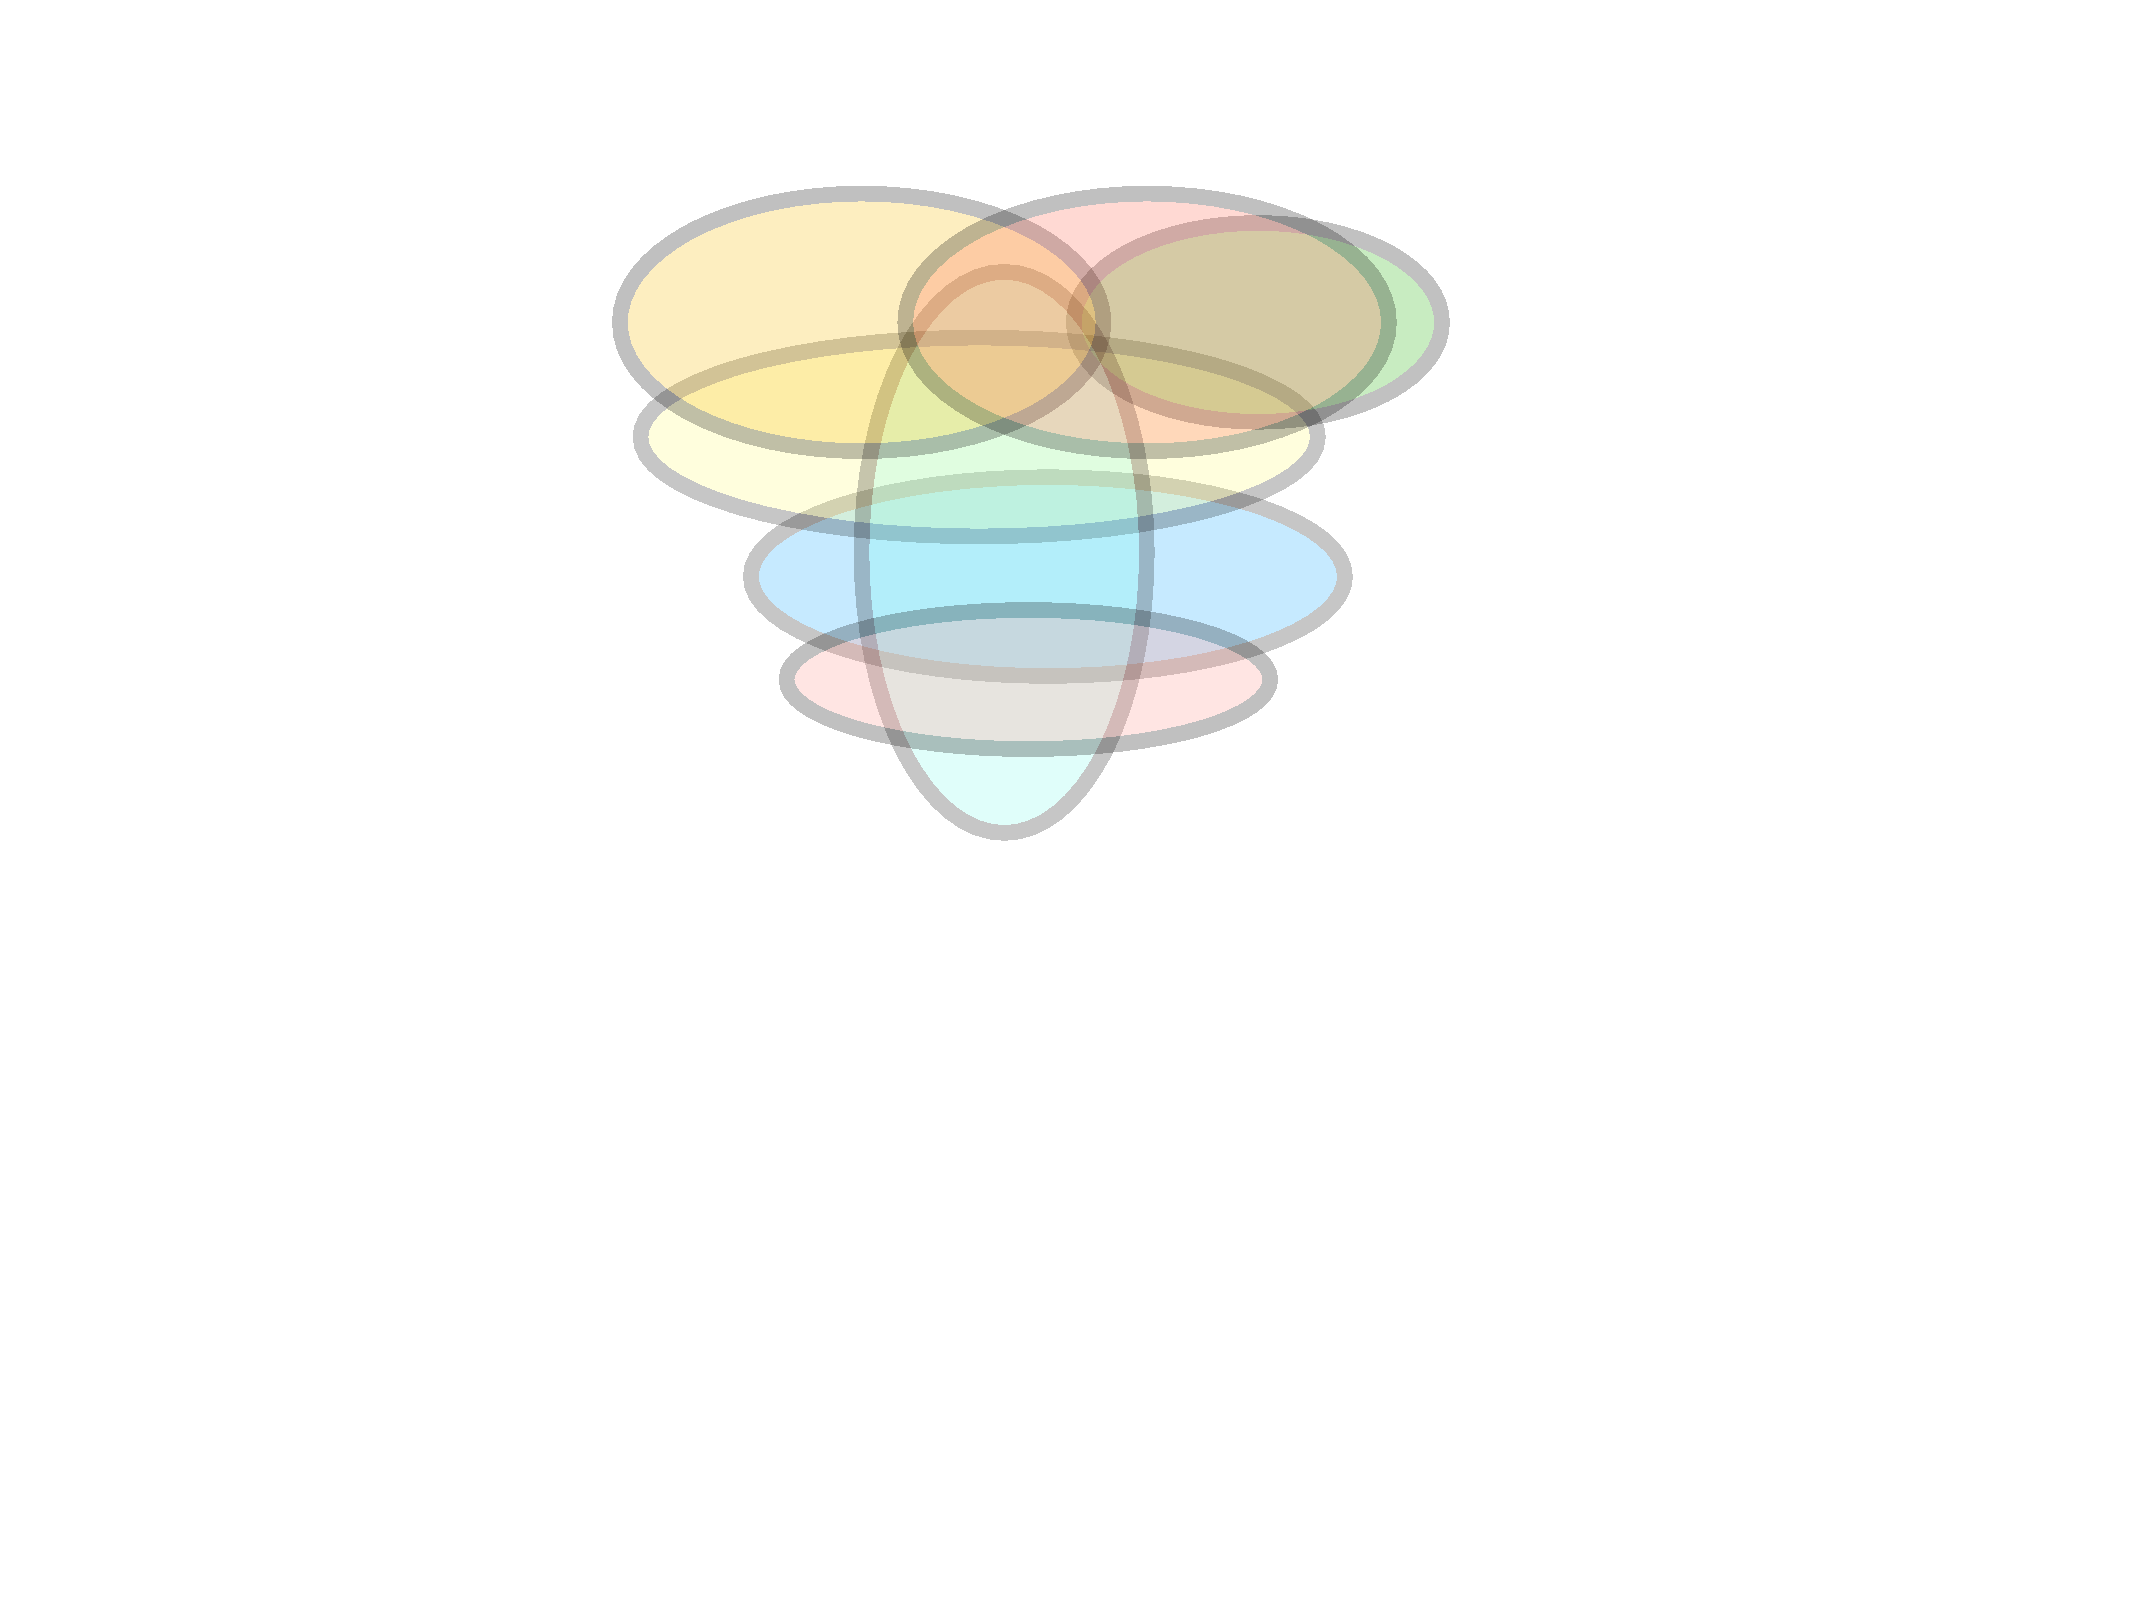
\includegraphics[width=\linewidth, trim=250  320 260 60,clip]{diagrams/Suff.pdf}
\end{minipage}
 & \ \ \ & 
\begin{minipage}{0.25\textwidth}
 
\includegraphics[width=\linewidth, trim=250  320 260 60,clip]{diagrams/Nec.pdf}
\end{minipage}
 & \ \ \ &
\begin{minipage}{0.25\textwidth}
 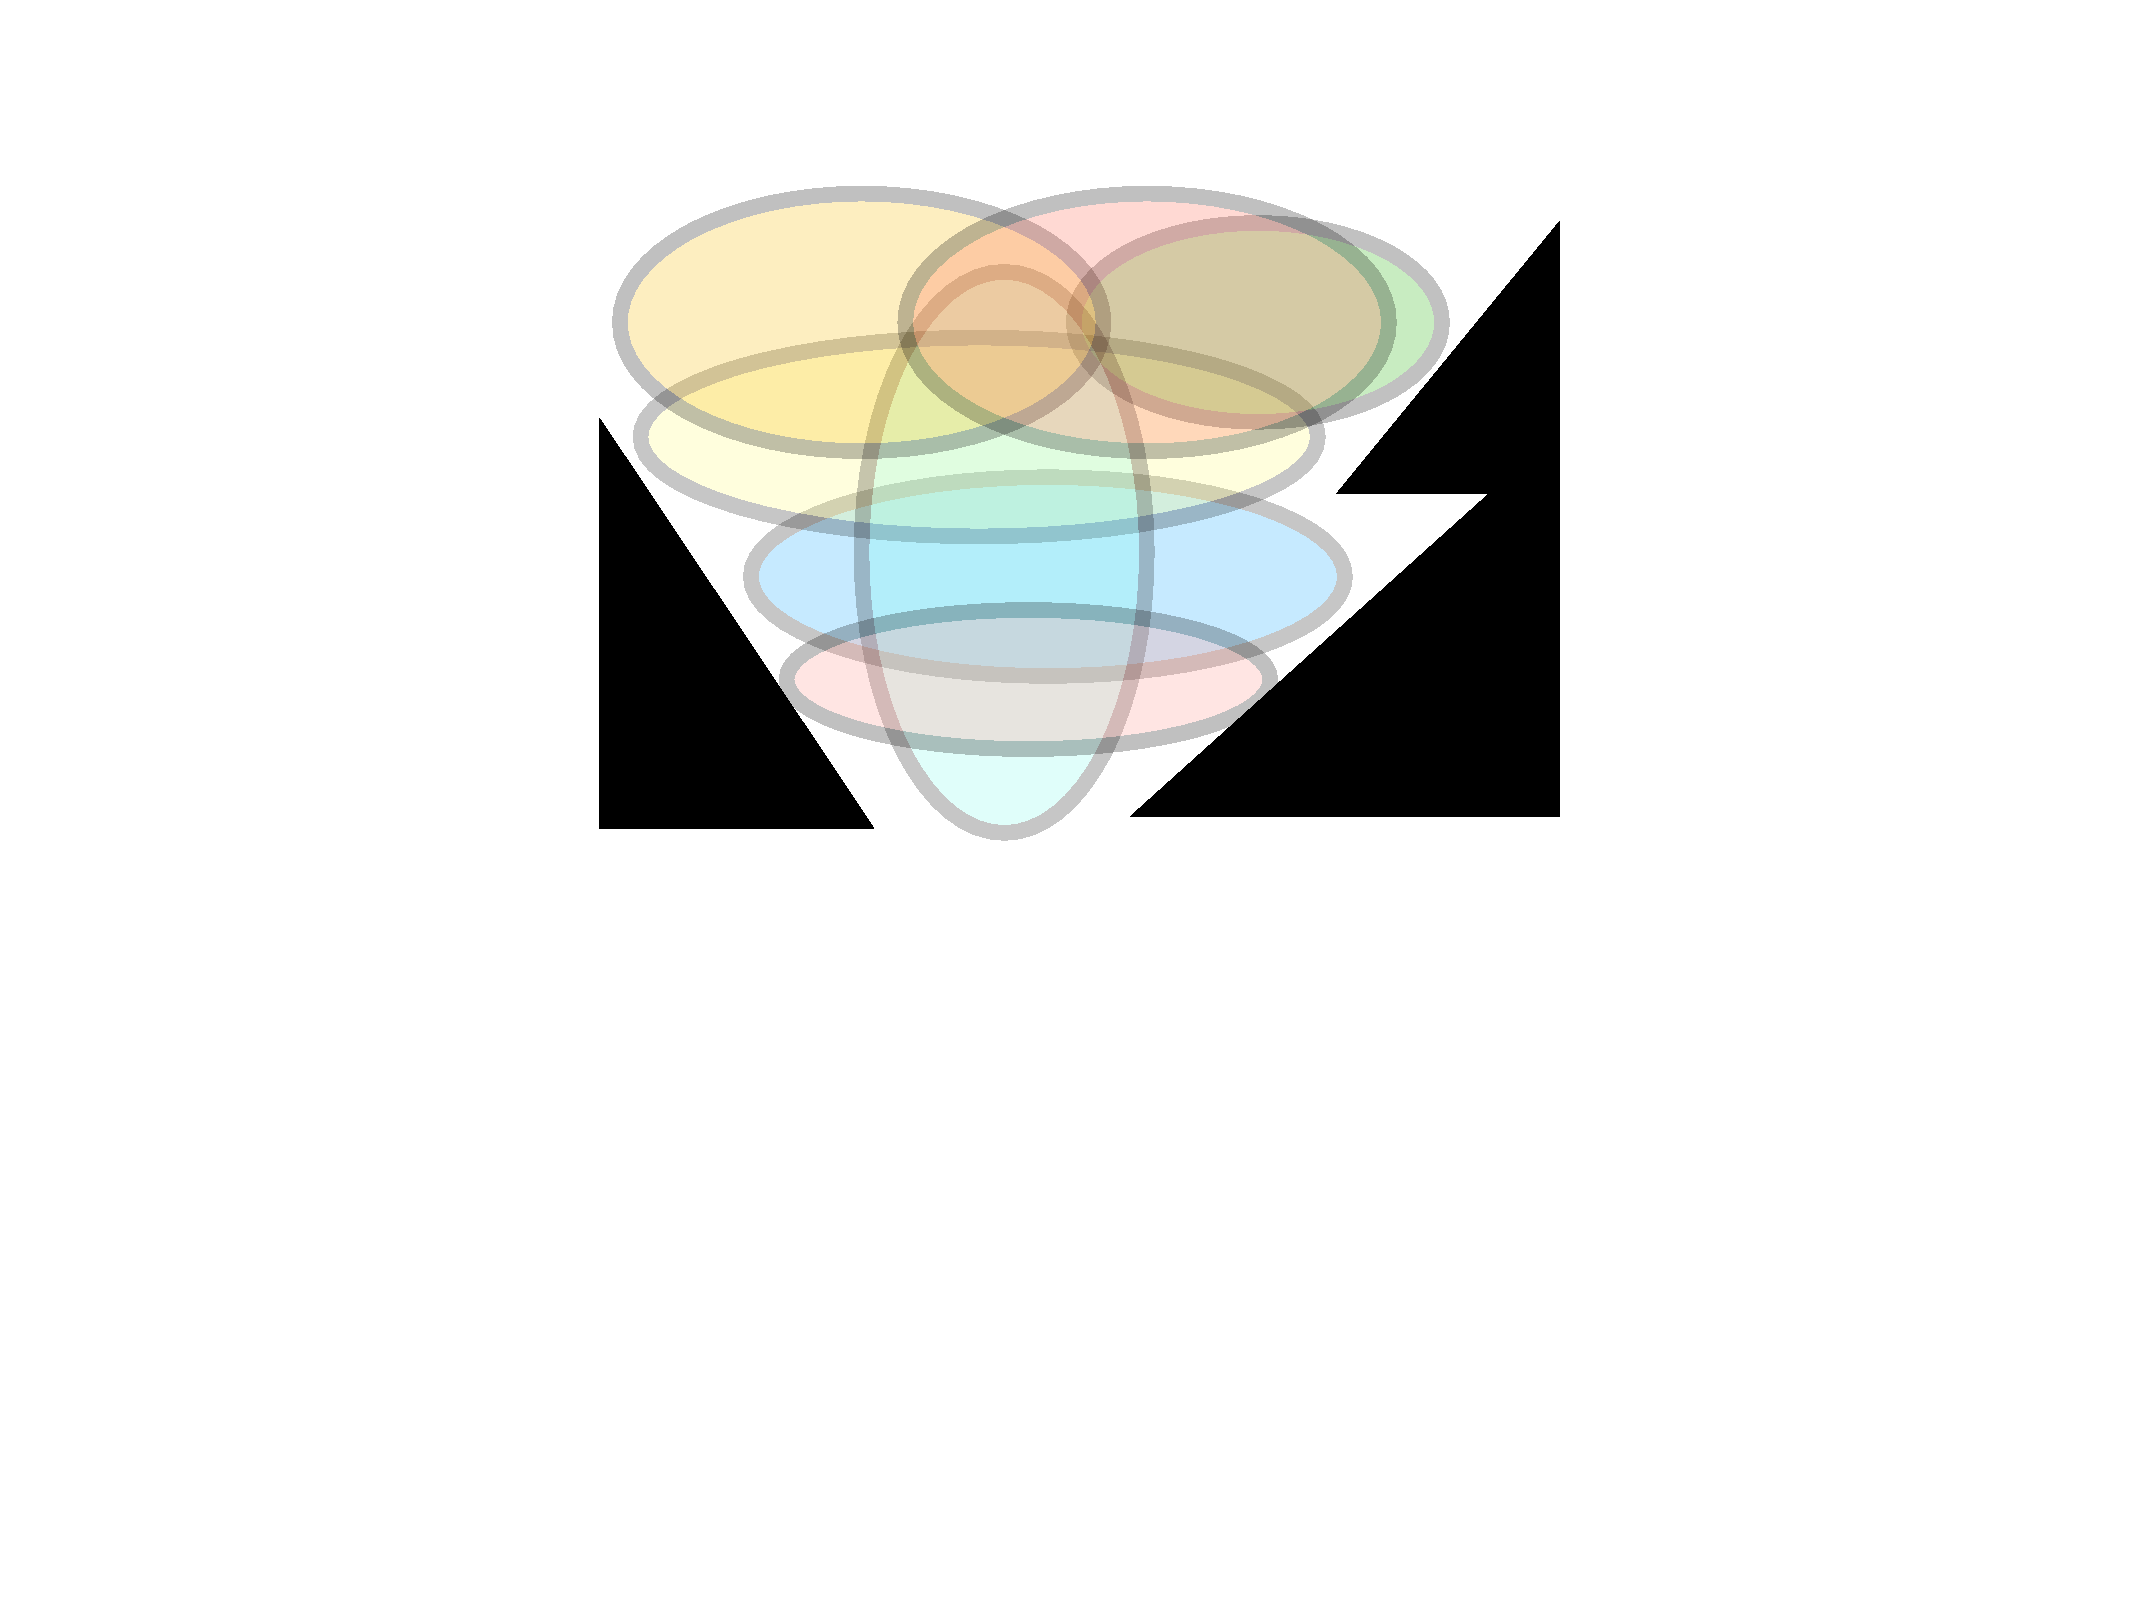
\includegraphics[width=\linewidth, trim=250  320 260 60,clip]{diagrams/NecAndSuff.pdf}
\end{minipage}
\\
sufficient  spec.& & necessary spec. & & holistic spec.
%\begin{minipage}{0.75\textwidth}
%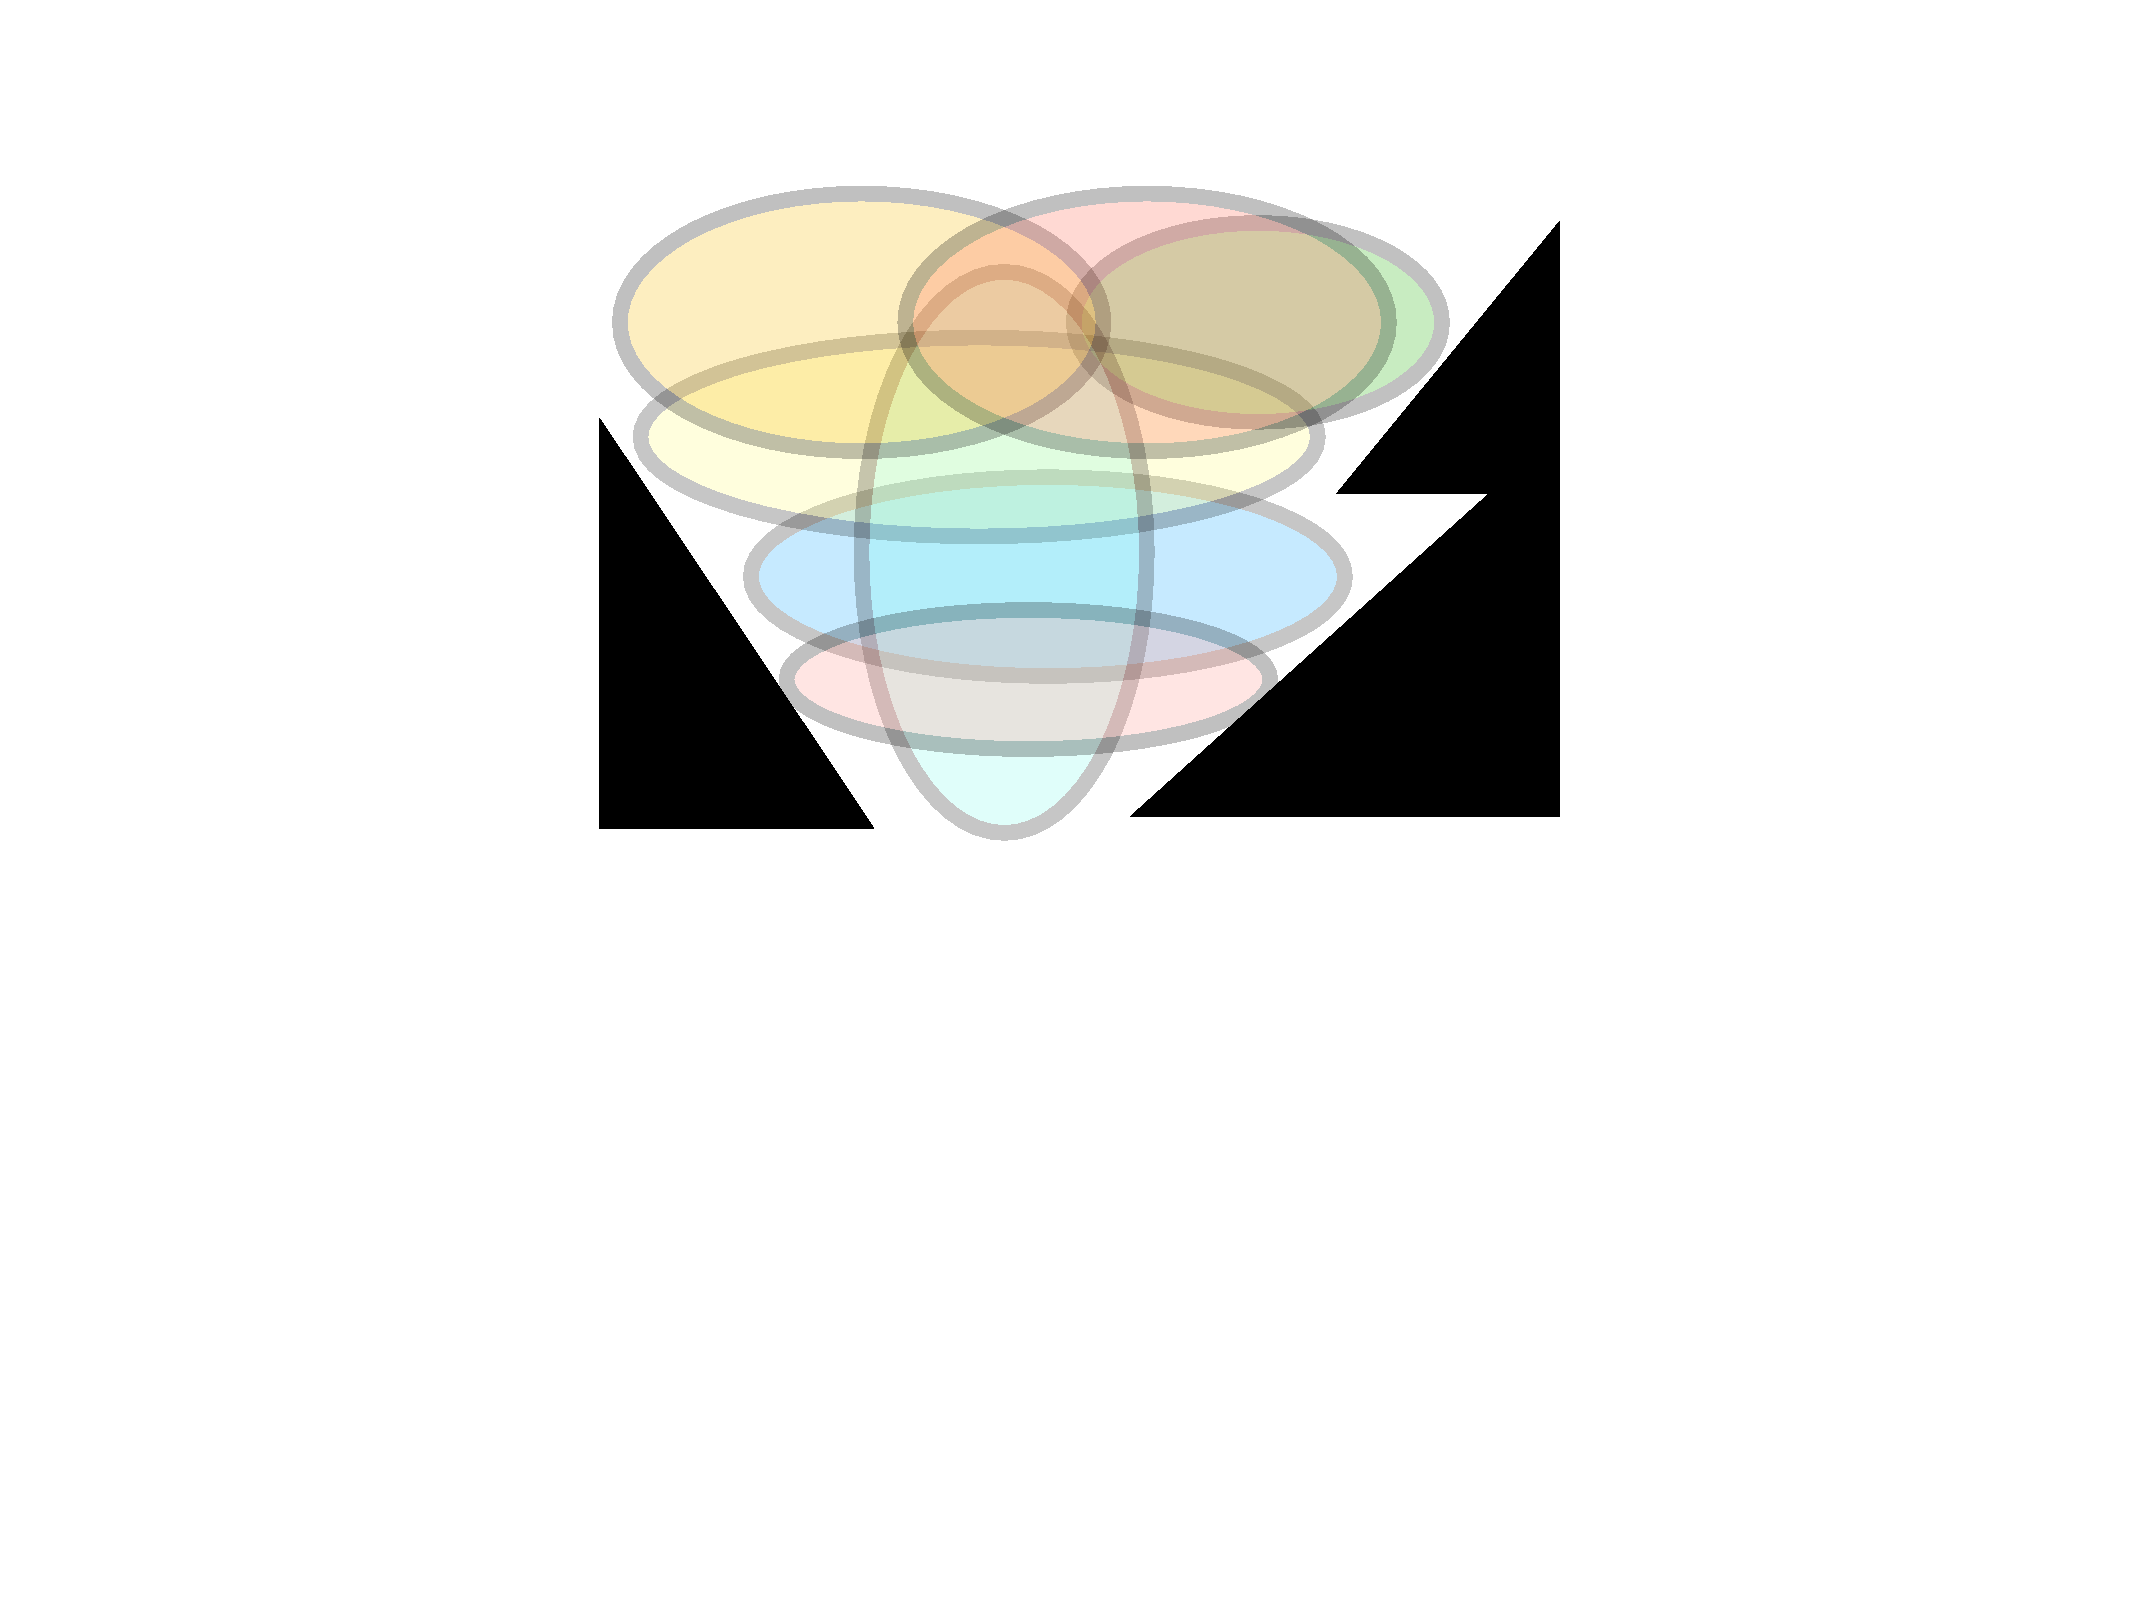
\includegraphics[width=\linewidth, trim=145  320 60 105,clip]{diagrams/NecAndSuff.pdf}
%\end{minipage}
%% y seems to eat up the bollom
%% x eats space from left, if you increase it the diagram decreases from left
%% w eats space from top, if you increase it the diagram decreases from top
%%\includegraphics[page=3, width=\linewidth, trim=150  270 40 150, clip]{diagrams/snmallocf.pdf}
%\sdcomment\sophia{I think we need to change the diagram so that it says small slab.}
%\end{minipage}
 \end{tabular}
  \vspace*{-2.5mm}
  \caption{Sufficient and Necessary Conditions, and Full Specifications}
 \label{fig:NecessaryAndSuff}
 \end{figure}
 
 We propose that  necessary conditions should be stated
 explicitly. Specifications should be \emph{holistic}, in the sense
 that they describe the  overall behaviour of a component: not only the
 behaviour of each individual functions, but also the 
 behaviour that emerges through combinations of functions.

Holistic specifications should therefore consist of   the sufficient as well as the necessary conditions, as  
depicted in right hand side  diagram in Fig. \ref{fig:NecessaryAndSuff}.
When a component has been specified holistically,  the behaviours
represented by the black triangles cannot occur, even when the
component interacts with other software of unknown provenance.
In Section \ref{sec:discussion} we argue why necessary conditions are more than the complement of
sufficient conditions.

Necessary conditions are guarantees upheld throughout program execution.
In this way, 
necessary conditions are closer to monitor or object
invariants \cite{Hoare74,Meyer97}. The difference between 
classical invariants and our holistic specifications is that classical invariants can only reflect  on
the current program state (\ie the contents of the
stack frame and the heap for an individual program component) while
holistic specifications reflect on all aspects of a program's
execution, potentially across all the components making up that program.


In this paper we propose \Chainmail, a specification language to
express holistic specifications.
%\james{has moved things around through here}
The design of \Chainmail was guided by the study of a sequence of
examples from the OCAP literature and the smart contracts world: the
membrane \cite{membranesJavascript}, the DOM \cite{dd,ddd}, the Mint/Purse \cite{MillerPhD}, the Escrow \cite{FTfJP14}, the DAO \cite{Dao,DaoBug} and
ERC20 \cite{ERC20}.  As we worked through the
examples, we found a small set of language constructs that let us
write holistic specifications across a range of different contexts.
%
 
While many individual features of \Chainmail can be found in other work, 
their power and novelty for specifying open systems lies in their careful combination.
In particular, \Chainmail extends 
traditional program specification languages\cite{Leavens-etal07,Meyer92} with features which talk about:
%
%\begin{description}
%\item[Permission] 
\ \ \textbullet \ \emph{Permission}, \ie which object may have access to which other objects; 
this is central since access to an object usually also grants access to the functions it provides.
%
\ \ \textbullet  \ \emph{Control}, \ie what  object called functions on other objects; this
 is useful in identifying the causes of certain effects - eg 
funds can only be reduced if the owner called a payment function.
%
%$\bullet$ \ \\emph{Authority}, \ie  which objects' state or properties may change; this is useful in describing effects, such as reduction of funds.
%
\ \ \textbullet \ \emph{Time}:\   \ie  what holds some time in  the past, the future, and what changes with time,
\ \ \textbullet \ \emph{Space}:\ \ie  which parts of the heap are considered when establishing some property, or when 
performing program execution; a concept
related to, but different from, memory footprints and separation logics,
\ \ \textbullet \ \sd{\emph{Viewpoints}:\ \ie  a distinction between the objects internal to our component, and those external to
it; a concept related to the open world setting.}
%\sophia{I do not know who wrote the comparison with foorprints, but it looks good to me.}
% end{description}

Holistic assertions often use several of these concepts. They often have the form of a guarantee
that if some property ever holds in the future, then some other property holds now, or that
certain effects can only caused by external objects with access to internal ones. \sophia{the first 4 sentences of this
para had been removed. But I modified them and like them. Waht do the others think?}
For example, if within a certain heap some change is possible in the future, then this particular heap contains 
at least one object which has access to a specific other, privileged object.
%\james{moved around --- not sure we need this para}
%\susan{I think we don't so there is a paragraph I have commented out.}
\forget{Ofte, holistic assertions typically have the form of a guarantee
that if some property ever holds in the future, then some other property holds now.
For example, if within a certain heap some change is possible in the future, then this particular heap contains 
at least one object which has access to a specific other, privileged object.}
A module\footnote{We use module and component in an analogous manner to class and object respectively.}
 satisfies a holistic assertion if, for all other modules,
  the assertion is satisfied  in all runtime configurations reachable through execution of the two modules combined.
  This reflects the open-world view.


\noindent The contributions of this paper are:\james{can we claim each of these?}\sophia{Yes to all, except for the last one --
not done yet. Do you think not?}
\begin{itemize}
\item the design of the holistic specification language \Chainmail,
\item the semantics of \Chainmail,
\item a validation of \Chainmail through its application to a sequence of examples,
\item a further validation of \Chainmail through informal proofs of adherence of code to some of these specifications.
\end{itemize}  
  
  
The rest of the paper is organized as follows: Section~\ref{sect:motivate:Bank} 
motivates our work in terms of an example. Sections~\ref{sect:LangOO} contain a formal definition of \LangOO, and Section~\ref{sect:assertions} the semantics of assertions. Section ... related work .... Section xxxx concludes.
\kjx{TODO AT THE END}




% \subsection{Conventions} 
\section{Motivating Example -- Attenuating the DOM}
\label{sect:mitave:DOM}
%We will now discuss  an example demonstrating the need to describe attenuation in specifications.
\emph{Attenuation} is ability to provide an untrusted client \emph{restricted}  access to an object's functionality. This is usually achieved through the introduction of an intermediate object. Such intermediate objects --- protection proxies \cite{gof} --- are a common design pattern, and their security properties and have been studied at length in the object capabilities literature \cite{millerPhD,murray10-infoflow}, and 
Devrise et. al. proposed specifications for attenuation for the DOM \cite{dd}.

In this section we revisit that example, and use it to motivate the
need for holistic specifications, and to give an informal introduction
to our for holistic  language Chainmail II. We also argue that
compared with Devrise et al., our specifications xxxx.\sdcomment{TO COMPLETE}.

This example deals with a tree of DOM nodes. Access to a DOM node
gives access to all its parent and children nodes, and the ability to
modify the properties of any accessible node. As the top nodes of the
tree usually contain privileged information (such as web content
showing your banking details), while the lower nodes contain less
crucial information (such as advertisements for BREXIT), we want to be
able to limit access given to third parties to only the lower part of
the DOM tree, (so that Jacob Rees-Mogg cannot access your bank
account). We do this via attenuation through a \prg{Wrapper}, which has
a field \prg{node} pointing to a \prg{Node}, and a field \prg{height}
which restricts the range of \prg{Node}s which may be modified through
the use of the particular \prg{Wrapper}. Namely, when you hold
a \prg{Wrapper} you can modify the \prg{property} of all the
descendants of the \prg{height}-th ancestors of the \prg{node} of that
particular \prg{Wrapper}.  It is not difficult to write such
a \prg{Wrapper}; a possible implementation appears in
Figure \ref{fig:DOM} in appendix \ref{DOM:traditional}.


Figure \ref{fig:WrapperUse} shows  
\prg{Wrapper} objects    attenuating the use of 
\prg{Node}s.
The
function \prg{usingWrappers} has as parameter an object of unknown
provenance, here called \prg{unknwn}. On lines 2-7 we create a tree
consisting of nodes \prg{n1}, \prg{n2}, ... \prg{n6}, depicted as blue
circles on the right-hand-side of the Figure. On line 8 we create a
wrapper of \prg{n5} with height \prg{1}. This means that the
wrapper \prg{w} may be used to modify \prg{n3}, \prg{n5} and \prg{n6}
(\ie the objects in the green triangle), while it cannot be used to
modify \prg{n1}, \prg{n2}, and \prg{4} (\ie the objects within the
blue triangle).  On line 8 we call a function named \prg{untrusted} on
the \prg{unknown} object, and pass \prg{w} as argument.

\begin{figure}[htb]
\begin{tabular}{llll}
\ \ &
\begin{minipage}{0.45\textwidth}
\begin{lstlisting}
func usingWrappers(unknwn){
   n1=Node(null,"fixed"); 
   n2=Node(n1,"robust"); 
   n3=Node(n2,"volatile"); 
   n4=Node(n2,"const");
   n5=Node(n3,"variable");
   n6=Node(n3,"ethereal");
   w=Wrapper(n5,1);
   
   unknwn.untrusted(w);
   
   assert n2.property=="robust" 
   ...
}
\end{lstlisting}
\end{minipage}
& & 
\begin{minipage}{0.75\textwidth}
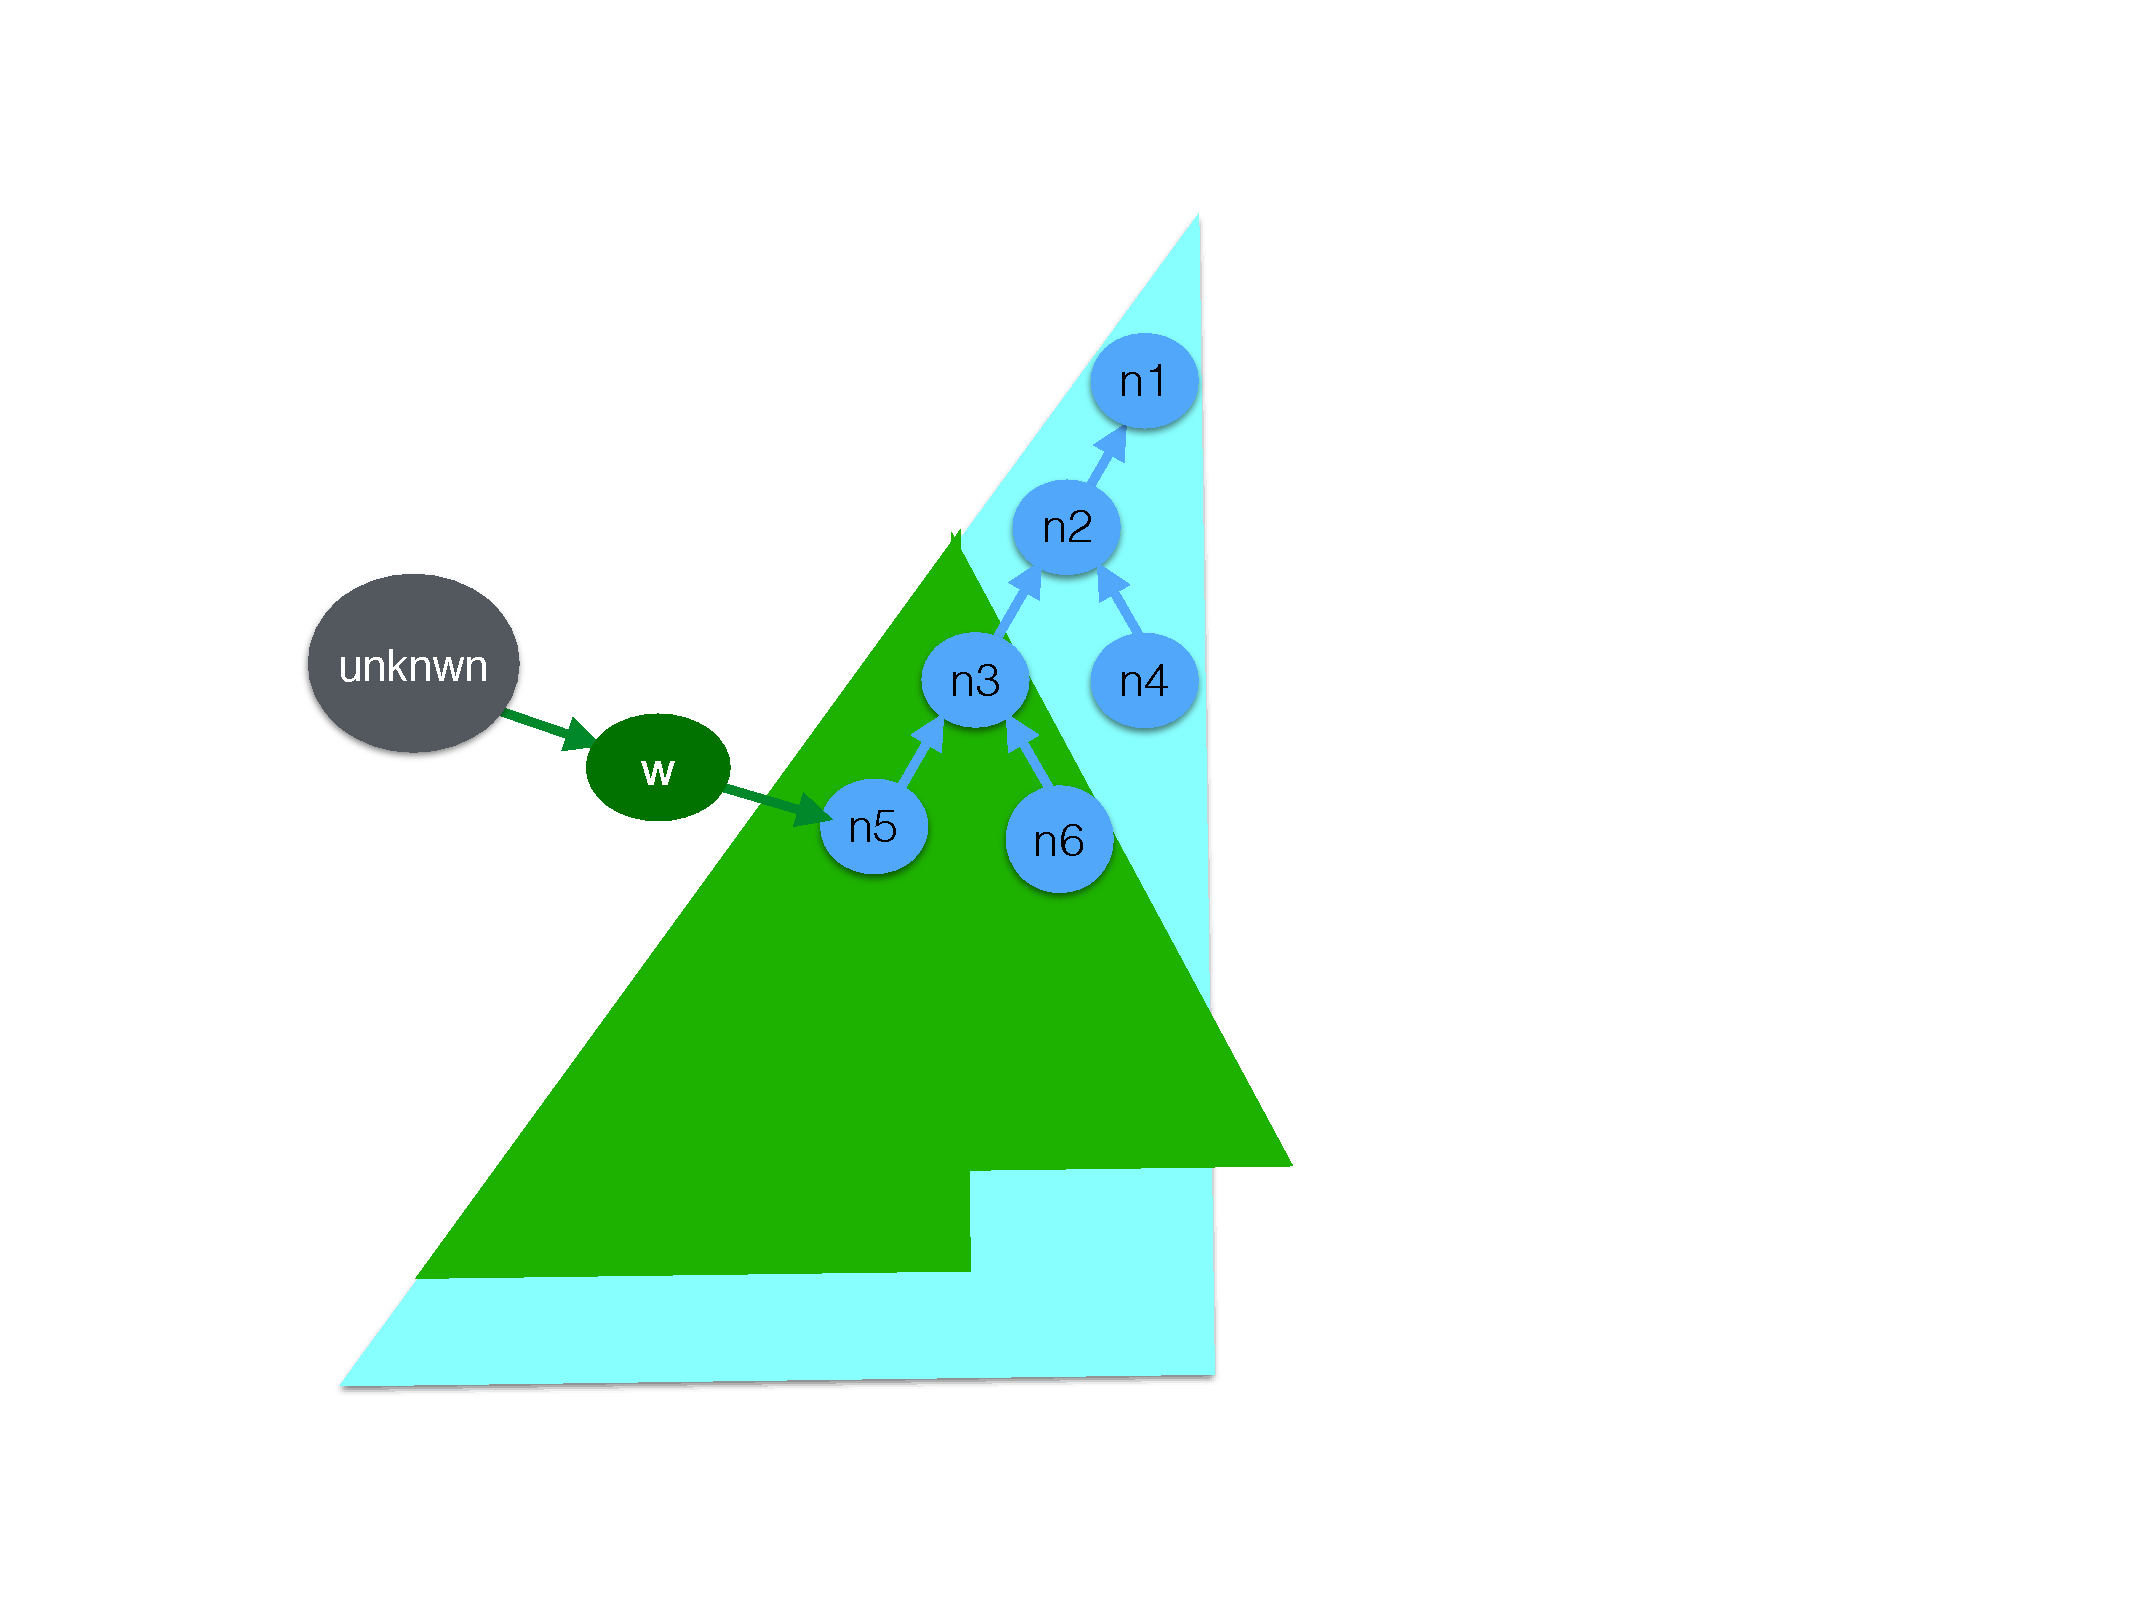
\includegraphics[width=\linewidth, trim=145  320 60 105,clip]{diagrams/DOM.pdf}
% x y z w
% y seems to eat up the bollom
% y=320 is good
% x eats space from left, if you increase it the diagram decreases from left
% w eats space from top, if you increase it the diagram decreases from top
% w=100 is good
%\includegraphics[page=3, width=\linewidth, trim=150  270 40 150, clip]{diagrams/snmalloc.pdf}\sdcomment{I think we need to change the diagram so that it says small slab.}
\strut \\
\strut \\

\end{minipage}
\end{tabular}
 \vspace*{-4.5mm}
\caption{\prg{Wrapper}s protecting \prg{Node}s }
\label{fig:WrapperUse}
\end{figure}

Even though we know nothing about the \prg{unknown} object or
its \prg{untrusted} function, and even though the call gives
to \prg{unknown} access to \prg{w}, which in turn has transitively
access to all \prg{Node}-s in the tree, we know that %the call to
the \prg{untrusted} function is guaranteed not to line 10 will not
affect the \prg{property} fields of the nodes \prg{n1}, \prg{n2},
and \prg{n4}.  Thus, the assertion on line 12 is guaranteed to
succeed.  The question is how do we specify \prg{Wrapper}, so as to be
able to make such an argument. %prove this assertion.

A specification of the class \prg{Wrapper} in the traditional
style, \eg \cite{Leavens-etal07} (\cf appendix \ref{DOM:traditional})
consists of pairs of pre- and post- conditions for each of the
functions of that class. Each such pair gives a {\em sufficient}
condition for some effect to take place: for example the
call \prg{w.setProperty(i,prp)} where \prg{i} is smaller
than \prg{w.height} is a sufficient condition to modify \prg{property}
of the \prg{i}-th parent of \prg{w.node}. But we do not know what
other ways there may be to modify a node's \prg{property}.  A broken
wrapper could accidently permit access to nodes one or two levels
about the expected height due to off-by one errors. More seriously,
a malicious wrapper could offer a
back-door public accessor method that leaks the underlying DOM
object through the wrapper, return direct access to any of the
other nodes in the DOM, or even to queue a task to
delete every property at midnight GMT on 29 March 2019. All of these errors are possible while
preserving the pre- and post- conditions expected of a \prg{Wrapper}. 
What is needed here is some way to specify the \emph{necessary
conditions}
under which some change could be made: if some external client is to
change a node's property, then  that client must have either direct
access to a node in that DOM tree, or indirect access via a wrapper
configured so that it can change the affected node.
Thus,
 \sdcomment{Shall we say the following, or does it break the flow?  
"Moreover, on line 10 we do not know which functions are called
on \prg{w}."
\kjx{I put that in and expanded on it. We need to explain the issues I think}
I do not see where it is}

% I think the below should be clear by niw
% In this work, we propose \emph{holistic specifications}, which
%describe the behaviour of an abstract data type as a whole, taking all
%possible method calls into account. Such holistic specifications
%emphasize the \emph{necessary conditions} for some effect to take
%place over the sufficient conditions as in traditional
%specifications. In our example:

\begin{quote}
The \emph{necessary} condition for the modification of \prg{nd.property} for some \prg{nd} of class \prg{Node}  is either access to some   \prg{Node} in the same tree, or  access to a \prg{w} of class \prg{Wrapper} where the \prg{w.height}-th parent of \prg{w} is an ancestor of \prg{nd}.
\end{quote}


With such a specification we can prove that the assertion on line 12
will succeed. Crucially, we can ensure that all future updates of
the \prg{Wrapper} class must continue to meet that specification,
guaranteeing the protection
of the \prg{Node} data. 
%
% Having justified the need for  necessary conditions in specifications, 
%
To give a flavour of \Chainmail, we use it  express the requirement from above:
%  This  gives us the opportunity to  demonstrate primitives for time ($\Future{\_}$) and authority ($\Changes{\_}$ and $\Using {\_} {\_}$).
 % and   more traditional relations between objects ( $\prg{nd}.\prg{parnt}^k\!=\! ...$):
% $\strut$ 
\vspace{.1cm}

\noindent
% \begin{quote}
$\forall \prg{S}:\prg{Set}.\forall \prg{nd}:\prg{Node}.\forall \prg{o}:\prg{Object}.$\\
$[\ \ {\Using{\Future {\Changes {\prg{nd.property}}}}  {\prg{S}}}$ \\
$\strut  \ \ \longrightarrow$\\
$\strut \ \ \ \exists \prg{o}.[\ \prg{o}\in\prg{S}\ \ \wedge\ \ \neg(\prg{o}:\prg{Node})\ \ \wedge\  \ \neg(\prg{o}:\prg{Wrapper})\ \ \ \wedge \  $\\
$ \strut\ \ \  \ \ \ \ \ \ \ \ [\ \exists \prg{nd}':\prg{Node}. \CanAccess{\prg{o}}{\prg{nd}'}\  \ \ \  \vee$\\
$ \strut\ \  \ \  \ \  \ \ \ \ \ \ \ \exists \prg{w}:\prg{Wrapper}.\exists k\!:\!\mathbb{N}.
% $\\ $ \strut \ \ \ \ \ \ \ \ \ \ \ \ \ \ \ \ \  \ \ \
  (\ \CanAccess{\prg{o}}{\prg{w}}  \ \wedge\ \prg{nd}.\prg{parnt}^k\!=\!\prg{w.node}.\prg{parnt}^{\prg{w.height}}) \ \ \ ]\ ]$\\
$ ]$
% \end{quote}

\vspace{.1cm}

% \noindent
That is, if the value of \prg{nd.property} is modified
($\Changes{\_}$) at some future point ($\Future{\_}$) and if reaching
that future point involves no more objects than those from set \prg{S}
(\ie ${\Using{\_} {\prg{S}}}$), then at least one (\prg{o}) of the
objects in \prg{S} is not a \prg{Node} nor a \prg{Wrapper},
and \prg{o} has direct access to some node
($\CanAccess{\prg{o}}{\prg{nd}'}$), or to some wrapper \prg{w} and
the \prg{w.height}-th parent of \prg{w} is an ancestor of \prg{nd}
(that is,
$\prg{parnt}^k\!=\!\prg{w.node}.\prg{parnt}^{\prg{w.height}}$).
% It is important to clarify what we mean by ``access''. 
Definitions of these concepts appear later
(Definition \ref{def:valid:assertion}), but note that our ``access''
is intransitive: $\CanAccess x y$ holds if either \prg{x} has a field
pointing to \prg{y}, or \prg{x} is the receiver and \prg{y} is one of
the arguments in the executing method call.
 
In the next sections we proceed with a formal model of our model. In the appendix we discuss more -- and simpler -- examples.
We chose the DOM for the introduction, in order to give a flavour of the \Chainmail features.
 



\section{Alternative Motivating Example: The Bank}
%\kjx{removed para that mostly duplicated intro}  
%% Traditional functional specifications describe what objects are
%% guaranteed to do. 
%% So long as a method is called in a state satisfying
%% its preconditions, the method will complete its work and establish a
%% state satisfying its postconditions.  
%% Thus, the precondition and the method call together form a \emph{sufficient}
%% condition for the method's effect.
% SD The below is wrong:
% Method specifications thus
% define the \textit{sufficient} conditions for their methods' behaviour
% to be invoked.

As a motivating example, we consider a simplified banking application,
with objects representing \prg{Account}s or \prg{Bank}s. 
As in \cite{ELang},   \prg{Account}s belong to \prg{Bank}s and hold money (here \prg{balance}s);  
with access  to two \prg{Account}s of the same  \prg{Bank} one can  transfer any amount of money from
 one to the other.  We give a traditional specification in Figure \ref{fig:BankSpec}.

%SD changed function to method, to fir what comes later.
\begin{figure}[htbp] 
\begin{lstlisting}
   method deposit(src, amt)
   PRE:  this,src:Account $\wedge$  this$\neq$src $\wedge$ this.myBank=src.myBank $\wedge$ 
         amt:$\mathbb{N}$  $\wedge$   src.balance$\geq$amt
   POST: src.balance=src.balance$\pre$-amt $\wedge$ this.balance=this.balance$\pre$+amt

   method makeNewAccount(amt)
   PRE: this:Account $\wedge$  amt:$\mathbb{N}$ $\wedge$  this.balance$\geq$amt
   POST: this.balance=this.balance$\pre$-amt $\wedge$ fresh result $\wedge$ 
         result: Account $\wedge$ this.myBank=result.myBank $\wedge$ result.balance=amt

   method newAccount(amt)
   PRE:  this:Bank  
   POST:  result: Account $\wedge$  result.myBank=this $\wedge$ result.balance=amt
 \end{lstlisting}
 \vspace{-.8cm}
\caption{Functional specification of \prg{Bank} and \prg{Account}
%
}
\label{fig:functionalSpecBankAccount}
\label{fig:BankSpec}
\end{figure} 

The PRE-condition of \prg{deposit} requires that  the receiver and the
first argument  (\prg{this} and \prg{scr}) are \prg{Account}s
and belong to the same bank,
that the second argument \prg{amt} is a number, and that \prg{src}'s
balance is least \prg{amt}.
The POST-condition mandates that \prg{amt} has been transferred from \prg{src} to the receiver.
 The function \prg{makeNewAccount}  returns a fresh \prg{Account} with the same bank, and transfers \prg{amt}
 from the receiver \prg{Account} to the new \prg{Account}.
 Finally, the function \prg{newAccount} when run by a \prg{Bank} creates a new \prg{Account} with corresponding 
 amount of money in it. \footnote{ \se{Note that our very simple bank doesn't even have a concept of owner of an account.}}
% \se{As specified in our \prg{BankSpec} the only way to put money into the \prg{Bank} is with a call to \prg{newAccount} and there is no way to remove money from the \prg{Bank}.}\sophia{We can say that, but is it important? We do not even use "newAccount" anywhere}

\forget{
\emph{Aside} Notice that the specification means that access to an \prg{Account} allows anyone to withdraw all the money it holds
-- the concept of account owner who has exclusive right of withdrawal is not supported.
This simplified view allows  us to keep the example short, but compare with appendix \sophia{TO ADD}
for a specification which supports owners. \emph{end aside}\sophia{which is the best place to say that?}
}

With such a specification %it is enough%to let us
%calculate the result of operations on the accounts ---
%for example % it is straightforward to determine that 
the code below  satisfies its assertion: assuming that 
\prg{acm\_acc} and \prg{auth\_acc} are \prg{Account}s for the ACM and
for a conference paper author respectively. The ACM's \prg{acm\_acc}
has a balance of 10,000 before an author is 
registered. but afterwards it has a balance of 11,000. Meanwhile the
\prg{auth\_acc}'s balance  will be 500 from a starting balance of 1,500
(barely enough to buy a round of drinks at the conference hotel bar).

\begin{lstlisting}
  assume acm_acc,auth_acc: Account $\wedge$ acm_acc.balance=10000 $\wedge$  auth_acc.balance=1500
  acm_acc.deposit(auth_acc,1000)
  assert acm_acc.balance=11000  $\wedge$ auth_acc.balance=500
\end{lstlisting}

\vspace{-.2in}

This reasoning is fine in a closed world, where we only have to
consider complete programs, where all the code in our programs (or any
other systems with which they interact) is under our control.   
In an
open world, however, things are more complex: our systems will be made
up of a range of 
%modules, 
components, many of which we do not control; and
furthermore will have to interact with external systems which we
certainly do not control.  Returning to our author, say some time
after registering by executing the \prg{deposit} code above, they
attempt to pay for a round at the bar.  Under what circumstances can
they be sure they have enough funds in their account?

To see the problem, what if the bank provided a \prg{steal} method that 
 emptied out every account in the bank into a thief's account.
 %\se{(also in the \prg{Bank})}?\sophia{yes, also in the bank, but does ti matter? I want to avoud having too many facets in the story.}
%all their funds into the thief's account.
%consider the additional function specified below.
% The bank additionally provides a
%\prg{steal} method that empties out every account in the bank and puts
%all their funds into the thief's account. 
If this method existed and
if it were somehow called between registering at the conference and
going to the bar, then the author 
%(actually everyone using the same bank)
%would find an empty account (as would every other account holder other than the thief, of course).
would find an empty account.
\susan{I have removed the statements that implied people had accounts because we don't have that in the spec}
%

%\vspace{-2in}
%\begin{lstlisting}
%   function steal(thief)
%   PRE:  this:Bank $\wedge$  thief.myBank=this 
%   POST: $\forall$a:Account.[a.myBank=this $\rightarrow$ a.balance=0 ] $\wedge$ 
%         thief.balance=thief.balance$\pre$+$\sum_{\prg{a}:\prg{Account} \wedge \prg{a.myBank}=\prg{this}}$ a.balance$\pre$
% \end{lstlisting}
%\vspace{-2in}
 
The critical problem is that a bank implementation including a \prg{steal}
method would meet the functional specification of the bank from
fig.~\ref{fig:functionalSpecBankAccount}, so long as the methods \prg{deposit},
\prg{makeNewAccount}, and \prg{newAccount}    meet
their specification.

One obvious solution would be to return to a closed-world
interpretation of specifications: we interpret specifications such as
fig.~\ref{fig:BankSpec} as \emph{exact} in the sense that only
implementations that meet the functional specification exactly,
\emph{with no extra methods or behaviour}, are considered as suitable
implementations of the functional specification. The problem is that
this solution is far too strong: it would for example rule out a bank
that  during software maintenance was given a new method \prg{count}
that simply counted the number of deposits that had taken place, or a method \prg{notify}
to enable the bank to occasionally send notifications  to its customers.
% occasionally paid interest to its clients.
%i.e. met fig.~\ref{fig:extras} as well as fig.~\ref{fig:BankSpec}.
%
%\begin{figure}[tbp]
%\begin{lstlisting}
%   function deposit(src, amt)
%   PRE:  $\mbox{ ... as before ...}$  
%   POST:  $\mbox{ ... as before ...}$  this.myBank.count=this.myBank.count$\pre$+1
% \end{lstlisting}
%\vspace{-.8cm}
%\caption{Counting deposits} %and paying interest}
%\label{fig:extras}
%\end{figure} 
% removed as payInterest affects the balance
%
%   function payInterest()
%   PRE: this:Bank  
%   POST: $\forall$a:Account.[a.myBank=this $\rightarrow$ a.balance=a.balance$\pre$+a.balance$\pre$/1000]


What we need is some way to permit bank implementations that 
%meet fig.~\ref{fig:extral} 
send notifications to customers but to forbid implementations of \prg{steal}. % that meet fig.~\ref{fig:steal}.  
The key here is to capture the (implicit)
assumptions underlying fig.~\ref{fig:BankSpec}, and to provide
additional specifications that capture those assumptions.  The following
 three informal requirements   prevent methods like \prg{steal}:

\begin{enumerate}
\item % After creation,
% it said
%  the \emph{only} way and account -- SD chnaged as I thibk ti has slifghtly wrong meaning 
An account's
  balance can be changed only  if a client   calls the \prg{deposit} method  with the
  account as the receiver or as an argument. 
 % \sophia{I changed the wording as I want to show "change -> call to deposit"}
%  \susan{point out that this is not sufficient to stop steal because it could be rewritten to use deposit.}
%  \sophia{I think that is what we say below}
\item An account's balance can be changed  only  if a client has
  access to that  particular account. % object.
  % I want the structure of (1) and (2) to be similar.
\item The \prg{Bank}/\prg{Account} component cannot leak access to existing accounts or banks. 
%SD I chnaged the belwo
%Neither accounts nor banks can leak money.   \susan{ I changed what you had in point 3 because it didn't make sense in context. I don't think what I put is what you were saying is it? Did you want to say something like 'There is no way that references to either accounts or banks can be passed to third parties?}
\end{enumerate}

Compared with the functional specification we have seen so far, these
requirements %assumptions 
capture \emph{necessary} %conditions 
rather than
\emph{sufficient} conditions:  Calling the \prg{deposit}
method to gain access to an account %is called to change an account's balance, and it is necessary
is necessary for any change to that account taking place.
%that the particular account object can be passed as a parameter to
%that method. 
The  function 
\prg{steal} is inconsistent with requirement  (1), as it reduces the balance of an \prg{Account} without calling the
function \prg{deposit}. 
However, requirement  (1) is not enough to protect our money. We need to (2) to avoid an \prg{Account}'s balance getting
modified without access to the particular \prg{Account}, and (3) to ensure that such accesses are not leaked. 

%\james{NEED TO DECIDE ON CONTRIBUTIONS.
%The contribution of this paper is a specification langauge and
%semantics that can be used to specify necessary specifications, and a
%semantics for those specifications that can determine whether some
%functional (sufficient) specifications are consistent (or not) with
%the necessary specifications. Also think that we do not do
%"can determine whether some
%functional (sufficient) specifications are consistent (or not) with
%the necessary specifications."}

 
We can  express these  requirements  %assumptions using 
through \Chainmail assertions.  Rather than %specifying \prg{functions} to  describe
specifying the behaviour of particular methods when they are called, we
write  invariants   that range across the entire behaviour of the
\prg{Bank}/\prg{Account}  module:
\vspace{.2cm}

%\begin{figure}[htbp]
%%\begin{definition}
%\label{def:pol2}

(1)\ \  $\triangleq$\ \ $\forall \prg{a}.[\ \ \prg{a}:\prg{Account} \wedge \Changes{\prg{a.balance}}  \ \    
    \longrightarrow \ \    \hfill$ \\
  $\strut \hspace{2.3cm} 
% TODO explain:
% we no longer need Past here, as we are ion visible states 
  \exists \prg{o}. [\    \Calls{\prg{o}}{\prg{deposit}}{\prg{a}}{\_} \vee\  \Calls{\prg{o}}{\prg{deposit}}{\_}{\prg{a}}\  \ ] \ \ \ \ ] \hfill $

\vspace{.4cm}

    (2)\ \  $\triangleq$\ \ $\forall \prg{a}.\forall \prg{S}:\prg{Set}.\ [  \ \  \prg{a}:\prg{Account}\ \wedge \  \Using{ \Future{\,\Changes{\prg{a.balance}}} \,}{\prg{S}\,}\ \ \   \
    \longrightarrow$ \\
 $\strut \hspace{3.9cm} \hfill \exists \prg{o}.\ [\, \prg{o}\in \prg{S}\ \wedge\  \External{\prg{o}}  \ \wedge \ \CanAccess{\prg{o}}{\prg{a}} \, ] \ \ \ \ ]$
\vspace{.4cm} 
 
     (3)\ \  $\triangleq$\ \ $\forall \prg{a}.\forall \prg{S}:\prg{Set}.\ [ \ \  \prg{a}:\prg{Account}\ \wedge \ \ {\Using{\Future{\ \exists \prg{o}.[\ \External{\prg{o}} \ \wedge\ \CanAccess{\prg{o}}{\prg{a}}]}}{\SF}}$ \\  
 $\strut \hspace{3.9cm} \hfill   \longrightarrow \ \ \ \exists \prg{o}'.\ [\, \prg{o}'\in \prg{S}\  \wedge  \ \External{\prg{o}'}  \ \wedge \ \CanAccess{\prg{o}'}{\prg{a}}   \ ] \ \ \ \ ]$

%\end{definition}
%\vspace{-.2cm}
%\caption{Necessary specifications for \prg{deposit}}
%%\label{fig:nec}
% \end{figure}
\vspace{.2cm}

%% We will discuss the meaning of  \Chainmail assertions in more detail in the next sections, but 
%% give here a first impression, and discuss (1)-(3):
 
Assertion (1) %in fig.~\ref{fig:nec} says 
says that if   an account's balance changes
($\Changes{\prg{a.balance}}$),
then there must be some client object \prg{o}
that % in the past (${\Past{...}}$) 
called the \prg{deposit} method with \prg{a} as a receiver or as an argument 
($\Calls{\prg{o}} {\prg{deposit}} {\_} {\_}$).
\sophia{ explain in some later section on that  this assertion
implicilty gives   that \prg{o} is external \kjx{why: it explicitly says
``external(o)''}}
%bank and its associated accounts ($\prg{o} \notin\prg{Internal}(\prg{a})$)" -- and I have chopped it from
%the spec. This is because of the visible states :-)}
 
Assertion (2) similarly constrains any possible change to an 
account's balance: 
If at some future point the balance changes  (${\Future{\,\Changes{...}}}$),  % (${\Future{...}}$) %
and if this future change is observed with the state restricted to the objects from \SF~ (\ie $\Using{...}{\prg{S}}$), then 
at least one of these objects ($\prg{o}\in\SF$) is external to the \prg{Bank}/\prg{Account} system ($\External{\prg{o}}$) and 
has (direct) access to that account object
($\CanAccess{\prg{o}}{\prg{a}}$).
Notice that while the change in the \prg{balance} happens some time in the future,
the external object \prg{o} has access to \prg{a} in the \emph{current} state.
Notice also, that the object which makes the call to \prg{deposit} described in (1), and the object which 
has access to \prg{a} in the current state described in (2) need not be the same: It may well be that the
latter passes (indirectly) a reference to \prg{a} to the former, which then   makes the call
to \prg{deposit}.

It remains to think about how access to a \prg{Account} may be obtained. This is the remit of assertion (3): 
\sd{It} says that if at \sd{some time} in the future of the state restricted to \SF, 
some object \prg{o} which is external has access to some account \prg{a}, and if \prg{a} exists in the 
current state, then in the current state some object 
from \SF~has access to \prg{a}. Note that \prg{o} and $\prg{o}'$ may but need not be the same object. Note also
that $\prg{o}'$ has to exist and have access to \prg{a} in the current state, but 
\prg{o} need not exist in the current state -- it may be allocated later.

\vspace{.1cm}

A  holistic  specification for the bank account, then,
would be our original sufficient functional specification from
fig.~\ref{fig:BankSpec} plus the necessary
%security policy
specifications (1)-(3) from above. %in fig.~\ref{fig:necBank}.   
This holistic specification
permits an implementation of the bank that also provides  \prg{count}
and \prg{notify} methods: the specification does not mention either method.
Critically, though, the \Chainmail specification
does not permit an
%specification from fig.~\ref{fig:count},
implementation that includes a \prg{steal} method.
\sophia{We said this earlier, do we repeat? \kjx{no, cos this time we're
saying it in chainmail..?}} 
First, the \prg{steal} method clearly changes the balance of
every account in the bank, but policy (1) requires that any method
that changes the balance of any account must be called \prg{deposit}.
Second, the \prg{steal} method changes the balance of every account in
the system, and will do so without the caller having a reference to
most of those accounts, thus breaching policy (2).   
% SD chopped. unnecessary
%Note that \prg{steal} putting all the funds into the thief's account
%does not breach policy (2) with respect to the thief's own account,
%because that account is passed in as a parameter to the \prg{steal}
%method, and so the called of the \prg{steal} must have access to that
%account.
 
Assertion (3) gives essential protection when dealing with foreign, untrusted code.
% \sophia{I like the story of this paragraph. Please make more eloquent.}
\sophia{Assertion (3) is a corollary of (2), and thus actually superfluous -- do we say that?
Do we say the story just using (2)?}
\susan{I think having 1 and 2 would make it more complicated. You could have a footnote though that says actually you don't even need 3 as it is a corollary of 2}
When an \prg{Account} is given out to untrusted third parties, assertion (3) guarantees that
this \prg{Account} cannot be used to obtain access to further  \prg{Account}s. 
The \prg{ACM} does not trust its authors, and certainly does not want
to give them access to \prg{acm\_acc}, which contains all of
the \prg{ACM}'s money. Instead, in order to receive money, it will
pass a secondary account used for incoming funds, \prg{acm\_incoming},
into which an \prg{author}  will pay the fee, and from which the \prg{ACM} will transfer the money
back into the main \prg{acm\_acc}. Assertion (3) is crucial, because it guarantees that even 
malicious authors  could not use knowledge of  \prg{acm\_incoming} to obtain access to
the main \prg{acm\_acc} or any other account. %, to which she did not have access.

\forget{
\sd{Thus, we need to be able to argue, that  passing the \prg{acm\_incoming to some unknown object \prg{u},
with an unknown function \prg{mystery}, is guaranteed not to affect \prg{acm\_acc} , unless \prg{u} already has
access to \prg{acm\_acc} before the call. With holistic assertions we can make this argument formally, while
with traditional specifications we cannot.}}
}
 
\vspace{.1cm} 

In summary, our  necessary specifications are invariants that describe the
behaviour of a module as observed by its clients. 
\forget{in fact, in section XXX\sophia{TO ADD} we show two very different implementations
of the \prg{Bank}/\prg{Account} specification which also satisfy (1)-(3).}
Our invariants 
 can talk about space, time and control, and thus go beyond
%can be defined and interpreted independently of any particular
%implementation of a specification --- rather our policies constrain
%implementations, in just the same way as traditional functional
%specifications. 
 %This is in contrast to e.g.\ 
 class invariants, which can only
talk   about relations between the  values of the fields of the objects.
%\sophia{This is james' original point, made a bit more concrete. Please check whether it makes sense.}
% of a module.
% invariants across the implementation of an abstract, or
% abstraction functions, which link an abstract model to a concrete
% implementation of that model. 
As our invariants are (usually) independent of a concrete implementation details they do not constrain the code to a specific implementation.



\kjx{\textbf{all these points should (already) be made by the example - the
  first one probably as early as the intro}
 As we already stated, this work is devoted to the specification of code in the open world. For these we propose what we call {\em holistic specifications.}
%
We claim that the most pertinent aspects of behaviour in the open world
are   in terms of  {\em necessary} conditions (\eg what can cause -- what are necessary conditions for --
 the balance of an account to decrease), rather than sufficient conditions (\eg the owner of an account may
 call the \prg{transfer} function, and as a result the balance decreases).
Such necessary conditions are not attached to particular function calls or program points; they apply
throughout program execution.
Therefore, they are expressed through  {\em invariants} that can be observed throughout the lifetime of a program, rather than at specific points in program execution.
  }
 


\section{\Chainmail: Holistic Specifications in Open Worlds}

%KJX In this section we give a brief overview of the most salient features of our approach, and give a full exposition in the next two sections.

\kjx{stuff shamlessly copied in from unplublisghed chainmail rejecta}

In this section we introduce our specification language \Chainmail,
and describe how it can be used to write holistic specifications.
We define \Chainmail's semantics formally below 
sections~4~to~7432 below.




  
Unlike JML or Dafny \cite{jml,daafny} \Chainmail specifications are not
tied tightly to the systems they are specifying. Rather, a system may
be described by a set of \Chainmail\ specifications, each consisting of
a number of named \lstinline+policy+ clauses.
\Chainmail\ specifications and policies overlap and are interlinked to
provide strong protection against attacks --- just like the links in
physical chainmail.  Each policy should aim to capture one very
specific concern in the design of a system. Traditional policies are
expressed as Hoare triples --- often describing a single method
invocation on an instance of the class being specified (as in
Figure~\ref{BANK-OR-DOM}).  Holistic policies are expressed as 
temporal or spatial invariants that a module that
conforms to the specification must maintain even though any other code
may be executed (as in policy FOO in Figure~\ref{DOM-OR-BANK}).

%% \Chainmail\ policies (and specifications) can cross cut both each
%% other and the various modules and objects in the system being
%% specified.  The validity of a specification is the conjunction of its
%% policies; a module or an object must satisfy all the specification's
%% policies for us to consider that the object meets the specification.
%% Policies and specifications are not tied to any specific module or
%% class: rather, any implementing module that satisfies the
%% specification's policies obeys the specification.


\Chainmail can express necessary specifications because its invariant
language includes \kjx{several carefully-chosen} \textit{holistic}
assertion constructs, along with traditional state-based assertions.
\kjx{if we say things like that, need to discuss alternative
  constructs in the discussion section. do we have alternatives?
  transitive Access. two-state assertions. what else?}.
That is, as well as supporting assertions on the contents of local
variabes and object fields (\eg $\prg{x}.\f1 > \prg{this}.\f2$),
\Chainmail\ incorporates assertions which talk about
%
\textit{access}
--- objects being accessible from other objects (\eg
$\CanAccess{\x}{\y}$);
%
\textit{control} --- the
next method to be invoked ($\Calls {\x} {\y} {\m} {\z}$);
%
\textit{authority} --- about the change of some
property (\eg $\Changes{\x.\f}$);
%
\textit{space} --- some property being observable within a subset of
the current state ( $\Using{\A}{S}$);
%
and
%
\textit{time} --- about some property
holding in the future or in the past (\eg $\Future \A$ or $\Past \A$).
%
.
\scd{While
many  individual
features of \Chainmail can  be found also in other work, we
%claim that their  combination as well as
%their application in the specification of open systems are novel.
argue that their power and novelty for specifying open systems lies in their careful
  combination}\kjx{Hmm. a delicate, subtle argument\ldots }
%
%
These assertions draw from some concepts from object capabilities
($\CanAccess{\_}{\_}$  for  permission and $\Changes{\_}$ for
authority) 
as well as temporal logic ($\Future \A$, $\Past \A$ and friends), and the relation of
our spatial connective ($\Using{\A}{S}$)  with ownership and effect
systems.\scd{TODO: add references here}. \kjx{don't forget the whole
  AOP mionitoring/specs stuff, just for fun.  (HELM contracts!!! (vs
  Meyer Contracts :-)}  
%
\kjx{somerwhere, should we say something like: the goal is
  to allow wholistic specifations with as extra little machinery as
  possible over a basic Hoare language}.

\subsection{Permission: Access}

Our first holistic assertion $\CanAccess{\x}{\y}$ asserts that one
object $\x$ has a direct reference to another object $\y$: that a
reference to $\y$ is the value of at least one of $\x$'s fields.
This assertion can be used to make assertions about heap structures (and thus
object values), for example that if a \prg{cacheValid} field is true,
then that object can access to a cached value:

\begin{lstlisting}
  a.cacheValid == true `$\weakImplies \CanAccess(a)(cacheValue)$` 
\end{lstlisting}

\kjx{do we really not also need reachable (transitive closure of access)}


\subsection{Control: Calls}

The  $\Calls {\x} {\y} {\m} {\z}$
assertion is more-or-less the control flow analogue of
the access assertion, and is true 
in program states where a method on object 
${\x}$ makes a method call ${\y}.{\m}({\z})$ --- that is it calls method 
{\m} on object {\y} with arguments {\z}.


\begin{lstlisting}
   another illustrative example, presumably in the context of the
   running example from the intro. which we need to pick first.
\end{lstlisting}


\subsection{Authority Changes}

The $\Changes{\x.\f}$  assertion is true when the value of \prg{x.f}
in the next state is different to the value in the current state.
For example, we 

\begin{lstlisting}
   another illustrative example, presumably in the context of the
   running example from the intro. which we need to pick first.
\end{lstlisting}

\subsection{Space: With}

The space assertionn $\Using{\A}{S}$ states the some assertion $\A$ is
true when the heap used by that assertion is restrcited to the
footprint $\S$  \kjx{footprint F?}.

\kjx{OK someone needs to explain what that's for and when/why it is sound to
do it}

\begin{lstlisting}
   another illustrative example, presumably in the context of the
   running example from the intro. which we need to pick first.
\end{lstlisting}


\subsection{Time: Next, Will, Prev, Was}

\Chainmail supports several temporal operators familiar from temporal
logic ($\Future \A$ or $\Past \A$ or $\Next \A$ or $\Prev \$A$). 
We support birectional temporal
assertions, constraining either future ($\Future \A$. $\Next \A$)
or past behaviour ($\Past \A$.  $\Prev \$A$) either considering only
the  immediate next or immediate previous step ($\Next \A$,
$\Prev \$A$) or for conditions that become eventually true in some
distant future, or were true once in some distant past  
($\Future \A$, $\Past \A$). We have bidirectional pairs of operators
to give expressiveness in writing assertions: this does not offer any
additional reasoning power. 

For example, a part of the observer pattern is that when
a subject is notified of a change, then the observer must
be told to update itself.    We can write this from the
subject's perspective, looking forwards:

\begin{lstlisting}
  Call(_,subject,notify,_) --> Will(Call(subject,observer,update,_))
\end{lstlisting}

\noindent meaning that once notify is called on a subejct, then its
observer will be updated sometime in the future.  We can write a very
similar specification for an observer, looking backwards.

\begin{lstlisting}
  Call(subject,observer,update,_) --> Was(Call(_,subject,notify,_))
\end{lstlisting}

\noindent meaning that if a subject updates an observer, that subject
have been notified somtime previously. We could tighten each
specifaction, so that the update must immediately follow the
notification, by replacing $\Future \A$ or $\Past \A$ with 
$\Next \A$ or $\Prev \A$.

\kjx{bother. should probably do time earlier, because most of the
   example assertions I can think of a things like
   \lstinline+(change(x.f) ->  past(call(_,xm,_)+

which needs the temporal opreator}


\kjx{OK really do need the example to be chosen to do more work here for this}


\subsection{The Open World}

\kjx{moved stuff about, only lightly touched. I'd want to down-rate
   this more, sophia would want to tighten everythign up}
   
To interpret \Chainmail\ specifications we need to have a model of the
programs whose behaviour they are specifying.
In our approach we represent code through modules ($\M$); these are
repositories of class definitions. \kjx{move to discussion: we use
classes, because we concentrate on class-based, object-oriented
programming; but we believe that the ideas are also applicable to
other kinds of languages}.  

We also use modules to model the crucial fact that our specifications
must hold ``in the open world'' --- that is, when our module may bhe
linked with \textit{arbitrary untrusted code}. To do this, we consider
the semantics of a module $\M$ as part of a pair
$\M \mkpair {\M'}$,  where $\M$ is the module 
whose code is supposed to satisfy the assertion,
and $\M'$, is \textit{any} module which exercises
the functionality of $\M$. We call $\M$ the {\em internal} module, while $\M'$ is the {\em external}
or {\em potentially adversarial} module. When examining program executions, we are interested
 in those runtime configurations which are {\em external} to module $\M$, \ie those where the
 executing object (\ie the current receiver) comes from module $\M'$.
 \footnote{\toby{TM: This looks like an \emph{excellent} way to handle this. Bravo. SD: :-)}}
 In  that sense, our approach is similar to that of visible states semantics, without, however the need to consider issues
around different objects of the same class or re-entrancy.\footnote{TODO: add references here.}



\kjx{wondered about moving this into the formal bit:}
  
The invariants are in the form of holistic assertions $\A$. We concentrate on what it means for a module to satisfy an assertion $\A$; we model this through the judgment $\M \models \A$.
%The judgment $\M \models \A$
This holds if for all further modules $\M'$ and in  all runtime configurations $\sigma$ which may be obseved through execution of the code of $\M$ combined with that of $\M'$, the assertion $\A$ is satisfied. More formally, we define:\\
$~ \strut  \hspace{1.3in} \M \models \A \ \ \  \ \ \ \mbox{
if               } \ \ \  \ \ \   \forall \sigma\in\Arising
{\M \mkpair  {\M'}}. \ \M \mkpair  {\M'}, \sigma \models \A$.  \\
%
\kjx{keep this bit:}
In that sense, module {\M'}  represents all possible clients of {\M}; and as it is arbitrarily chosen, it reflects the open world nature of our specifications.


\section{The language \LangOO}
\label{sect:LangOO}

\subsection{Modules and Classes}
\label{secONE}

\LangOO programs are described through modules, which are repositories of code. Since we study class based oo languages,
code is represented as classes, and  modules are mappings from  identifiers to class  descriptions.

\begin{definition}[Modules]
\label{defONE}
We define $\syntax{Module}$ as  the set of mappings from identifiers to class descriptions (the latter defined in Definition \ref{def:syntax:classes}):\\  % to force line break

\begin{tabular}  {@{}l@{\,}c@{\,}ll}
\syntax{Module} \ \  &  \   $\triangleq $  \ &
   $ \{ \ \ \M \ \ \mid \ \  \M: \ \prg{Identifier} \   \longrightarrow \
  \  \syntax{ClassDescr}     \  \    \}$
 \end{tabular}
\end{definition}
 
Classes, as defined   below,
consist of field and method definitions.
Note that \LangOO is untyped. Method bodies consist of sequences of statements;
these can be field read or field assignments, object creation, method calls, and return statements.
All else, \eg booleans, conditionals, loops,  can be encoded.

Note also that field read or write is only allowed if the target object is \prg{this} -- as, \eg, as
  in Smalltalk -- this is encapsulation: the syntax allows an object to read/write its own fields, but
   forbids it from reading/writing any other object's fields.

\label{sec:syntax:classes}


\begin{definition}[Classes]
\label{def:syntax:classes}
We define the syntax of class descriptions below.

\begin{tabular}{lcll}
 \syntax{ClassDescr}   &   \BBC  &     \kwN{class}  \syntax{ClassId}    \lb\,  $($\ \kw{field} \f\ $)^*$ \
 $($  \kwN{method}\ \syntax{MethBody}\ $)^*$   \ \rb
\\
\syntax{MethBody} &\BBC&
       \m\lp \x$^*$\rp     \lb\, \syntax{Stmts}  \,
    \rb
 \\
 \syntax{Stmts}  &\BBC&  \syntax{Stmt}     ~\SOR~  \syntax{Stmt} \semi \syntax{Stmts} \\
\syntax{Stmt}    &\BBC&
       \kw{this}.\f {\kw{:=}} \x   ~\SOR~  \x{\kw{:=}}  \kw{this}.\f    ~\SOR~        \x  {\kw{:=}} \x.\m\lp \x$^*$\rp  \\
       & &    ~\SOR~     \x  {\kw{:=}}     \newKW\, \c\,\lp \x$^*$\rp   ~\SOR~
   \returnKW \,  \x   \\
 \x, \f, \m &\BBC&  \prg{Identifier}
 \end{tabular}

  \vspace{.03in}
  \noindent
 where we use metavariables as follows:
 $\x \in  \syntax{VarId} \ \ \  \f \in  \syntax{FldId} \ \ \  \m \in  \syntax{MethId} \ \ \  \c \in  \syntax{ClassId}$
\end{definition}


We define a method lookup function, $\mathcal{M}$ which returns the corresponding method definition given a class \c\ and a method identifier \m.


 \begin{definition}[Lookup] For a class identifier \prg{C}  and a method identifier \prg{m} : $ ~ $ \\

\noindent
$
\Meths {} {\prg{C}} {m}       \triangleq  \ \left\{
\begin{array}{l}
                        \m\, \lp \p_1, ... \p_n \rp \lb Stmts   \rb\\
\hspace{0.5in} \mbox{if}\  \M(\prg{C}) =   \kwN{class}\, \prg{C}\, \  \lb ...   \kwN{method}\ ...\  \m\, \lp \p_1, ... \p_n \rp \lb Stmts  \rb  ... \ \rb.
\\
\mbox{undefined},  \ \ \ \mbox{otherwise.}
\end{array}
                    \right.$

  \end{definition}

\subsection{The Operational Semantics of \LangOO}
\label{formal:semantics}

We will now define execution of \LangOO code.
We start by  defining the  runtime entities, and runtime configurations, $\sigma$, which consist of heaps and stacks of frames.
 The frames are pairs consisting of a continuation, and a mapping from identifiers to values.
The continuation represents the code to be executed next, and the mapping gives meaning
to the formal and local parameters.

\begin{definition}[Runtime Entities]
We define  addresses, values, frames, stacks, heaps and runtime configurations.

\begin{itemize}
\item
We take addresses to be an  enumerable set,  \prg{Addr}, and use the identifier $\alpha\in \prg{Addr}$ to indicate an address.
\item
Values, $v$, are either addresses, or sets of addresses or null:\\
 $~ ~ ~ \ v \in \{ \prg{null} \} \cup \prg{Addr}\cup {\mathcal P}( \prg{Addr})$.
\item
  Continuations are either   statements  (as defined in Definition~\ref{def:syntax:classes}) or a marker, \x {\kw{:=}} $\bullet$, for a nested call followed by
  statements to be executed
  once the call returns.


\begin{tabular}{lcll}
\syntax{Continuation} &\BBC&   \syntax{Stmts} ~\SOR~   \x {\kw{:=}} $\bullet$ \semi\ \syntax{Stmts} \\
 \end{tabular}

\item
Frames, $\phi$, consist of a code stub  and a  mapping from identifiers to values:\\  $~ ~ ~ \ \phi \ \in\ \syntax{CodeStub} \times \prg{Ident} \rightarrow Value$,
\item
Stacks,  $\psi$, are sequences of frames, $\psi\ ::=   \phi \ | \ \phi\cdot\psi$.
\item
Objects consist of a class identifier, and a partial mapping from field identifier to values: \\  \ $~ ~ ~ \ Object\ = \ \prg{ClassID} \times (\prg{FieldId} \rightarrow Value)$.
\item
Heaps, $\chi$, are mappings from addresses to objects:\  \  $\chi\ \in\ \prg{Addr} \rightarrow Object$.
\item
Runtime configurations, $\sigma$, are pairs of stacks and heaps, $\sigma\ ::=\ (\ \psi, \chi\ )$.
\end{itemize}

\end{definition}


Note that values may be sets of addresses. Such values are never part of the execution of \LangOO, but are used to give semantics to assertions -- we shall see that in Definition \ref{def:valid:assertion}.



Next, we define the interpretation of variables (\x) and   field look up  (\this.\f)
in the context of frames,
heaps and runtime configurations; these interpretations are used to define the operational semantics and  also  the
validity of assertions, later on in Definition \ref{def:valid:assertion}:

\begin{definition}[Interpretations]
We first define lookup of fields and classes, where $\alpha$ is an address, and \f\, is a field identifier:
\begin{itemize}
\item
$\chi ({\alpha},{\f})$ $\triangleq$  $\fldMap({\alpha},{\f})$\ \ \ if \ \ $\chi(\alpha)=(\_, \fldMap)$.
\item
$\ClassOf {\alpha} {\chi} $ $\triangleq$ $\c$\  \ \ if \ \ $\chi(\alpha)=(\c,\_)$
\end{itemize}

\noindent
We now define interpretations  as follows:

\begin{itemize}
\item
$\interp {\x}{\phi} $ $\triangleq$ $\phi(\x)$
\item
$\interp {\this.\f}{(\phi,\chi)} $ $\triangleq$ $v$, \ \ \ if \ \ $\chi(\phi(\this))=(\_, \fldMap)$ and $\fldMap(\f)$=$v$

\end{itemize}

\noindent
For ease of notation, we also use the shorthands below:
\begin{itemize}
\item
$\interp {\x}{(\phi\cdot\psi,\chi)} $ $\triangleq$ $\interp {\x}{\phi} $
\item
$\interp {\this.\f}{(\phi\cdot\psi,\chi)} $ $\triangleq$ $\interp  {\this.\f}{(\phi,\chi)} $
\item
$\ClassOf {\alpha} {(\psi,\chi)} $ $\triangleq$ $\ClassOf {\alpha} {\chi} $
\end{itemize}

\end{definition}

In the definition of the operational semantics of \LangOO we use the following notations for lookup and updates of runtime entities :

\begin{definition}[Lookup and update of runtime configurations]
We define convenient shorthands for looking up in  runtime entities.
\begin{itemize}
\item
Assuming that $\phi$ is the tuple  $(\prg{stub}, varMap)$, we use the notation  $\phi.\prg{contn}$ to obtain \prg{stub}.
\item
Assuming a value v, and that $\phi$ is the tuple  $(\prg{stub}, varMap)$, we define $\phi[\prg{contn}\mapsto\prg{stub'}]$ for updating the stub, \ie
$(\prg{stub'}, varMap)$.   We use  $\phi[\x \mapsto v]$  for updating the variable map, \ie  $(\prg{stub}, varMap[\x \mapsto v])$.
\item
Assuming a heap $\chi$, a value $v$, and   that $\chi(\alpha)=(\c, fieldMap)$,
we use $\chi[\alpha,\f \mapsto v]$ as a shorthand for updating the object, \ie $\chi[\alpha \mapsto (\c, fieldMap[\f \mapsto v]]$.
\end{itemize}

\end{definition}



\begin{figure*}
$\begin{array}{l}
\inferenceruleNN {methCall\_OS} {
\\
\phi.\prg{contn}\ =\ \x {\kw{:= }} \x_0.\m \lp \prg{par}_1, ... \prg{par}_n \rp \semi \prg{Stmts}
\\
\interp{\x_0}{\phi} = \alpha
\\
\Meths {} {\ClassOf {\alpha} {\chi}} {\m} \  =  \ \m\lp par_1, \ldots par_n \rp \lb \prg{Stmts}_1   \rb
  \\
 \phi''\ =\  (\  \prg{Stmts}_1,\ \ (\ \this \mapsto \alpha,
  \prg{par}_1 \mapsto  \interp{\x_1}{\phi}, \ldots \prg{par}_n \mapsto  \interp{\x_n}{\phi}\ ) \ )
}
{
 \M,\, (\ \phi\cdot\psi,\ \chi\ )\ \ \leadsto\  \ (\ \phi''\cdot\phi[\prg{contn}\mapsto\x  \kw{:=} \bullet \semi \prg{Stmts}] \cdot\psi,\ \chi\ )
}

\\ \\
\inferenceruleNN {varAssgn\_OS} {
 \phi.\prg{contn} \ = \ \x  {\kw{:= }}   \this.\f \ \semi \prg{Stmts}
}
{
 \M,\,  (\ \phi\cdot\psi, \chi\ )\ \ \leadsto\  \ (\ \phi[ \prg{contn} \mapsto \prg{Stmts}, \x\mapsto \interp{\this.\f}{\phi,\chi}] \cdot\psi,\ \chi\  )
}
\\
\\
\inferenceruleNN{fieldAssgn\_OS} {
 \phi.\prg{contn}\ =\  \this.\f  \kw{:=} \x  \semi \prg{Stmts}
}
{
 \M,\,  (\ \phi\cdot\psi, \chi\  )\ \ \leadsto\  \ (\ \phi[\prg{contn}\mapsto  \prg{Stmts} ] \cdot\psi, \chi[\interp{\this}{\phi},\f \mapsto \interp{\x}{\phi,\chi}]\  )
}
\\
\\
\inferenceruleNN {objCreate\_OS} {
 \phi.\prg{contn}\ =\  \x  \kw{:=} \kwN{new }\, \c \lp \x_1, ... \x_n \rp  \semi \prg{Stmts}
 \\
 \alpha\ \mbox{new in}\ \chi
 \\
\f_1, .. \f_n\ \mbox{are the fields declared in } \M(\c)
}
{
 \M,\,  (\ \phi\cdot\psi, \chi\ )\ \ \leadsto\  \ (\ \phi[\prg{contn}\mapsto  \prg{Stmts},\x \mapsto \alpha\ ] \cdot\psi, \ \chi[\alpha \mapsto (\c,\f_1 \mapsto \interp{\x_1}{\phi},  ... \f_n \mapsto \interp{\x_n}{\phi}  ) ]\ )
}
\\
\\
\inferenceruleNN {return\_OS} {
 \phi.\prg{contn}\ =\   {\kwN{return }}\, \x  \semi \prg{Stmts}\ \  \ or\  \ \  \phi.\prg{contn}\ =\   {\kwN{return}}\, \x
 \\
\phi'.\prg{contn}\ =\  \x' \kw{:=} \bullet  \semi \prg{Stmts}'
}
{
 \M,\,  (\ \phi\cdot\phi'\cdot\psi, \chi\ )\ \ \leadsto\  \ (\ \phi'[\prg{contn}\mapsto  \prg{Stmts'},\x' \mapsto \interp{\x}{\phi}] \cdot\psi, \ \chi \ )
}
\end{array}
$
\caption{Operational Semantics}
\label{fig:Execution}
\end{figure*}

Execution of a statement has the form $\M, \sigma \leadsto \sigma'$, it is defined in figure \ref{fig:Execution}.

\begin{definition}[Execution] of one or more steps is defined as follows:

\begin{itemize}
     \item
   The relation $\M, \sigma \leadsto \sigma'$, it is defined in Figure~\ref{fig:Execution}.

   \item
   $\M, \sigma \leadsto^* \sigma'$ holds, if a) $\sigma$=$\sigma'$, or b) there exists a $\sigma''$ such that
   $\M, \sigma \leadsto^* \sigma''$ and $\M, \sigma'' \leadsto \sigma'$.
 \end{itemize}

\end{definition}

\footnote{Toby had added that following but I do not see what we need it for. \toby{We defer the definition of initial configurations to Definition~\ref{defn:initial-and-arising} later.}}

\subsection{Definedness of execution, and extending configurations}

Note that interpretations and executions need not always be defined.
For example, in a configuration whose top frame does not contain \x\,  in its domain, $\interp {\x}{\phi} $ is undefined. We define the relation $\sigma \subconf \sigma'$ to express that   $\sigma$ has more information than $\sigma'$, and then prove that more defined configurations preserve interpretations:

\begin{definition}[Extending runtime configurations]
The relation $\subconf$   is defined on runtime configurations as follows. Take arbitrary
configurations $\sigma$, $\sigma'$, $\sigma''$, frame $\phi$, stacks $\psi$, $\psi'$,  heap $\chi$, address $\alpha$ free in $\chi$, value $v$ and object $o$, and define $\sigma  \subconf \sigma'$ as the smallest relation such that:

\begin{itemize}
\item
$\sigma  \subconf \sigma$
\item
$(\phi[\x \mapsto v]\cdot \psi, \chi) \subconf  (\phi\cdot \psi, \chi)$
\item
$(\phi\cdot\psi\cdot\psi', \chi) \subconf  (\phi\cdot \psi, \chi)$
\item
$(\phi, \chi[\alpha \mapsto o) \subconf  (\phi\cdot \psi, \chi)$
\item
$\sigma'  \subconf \sigma''$ and $\sigma''  \subconf \sigma$ imply $\sigma'  \subconf \sigma$
\end{itemize}
\end{definition}



\begin{lemma}[Preservation of interpretations and executions]
If $\sigma'  \subconf \sigma$, then

\begin{itemize}
\item
If $\interp {\x}{\sigma}$ is defined,\ \  then $\interp {\x}{\sigma'}$=$\interp {\x}{\sigma}$.
\item
If $\interp {\this.\f}{\sigma}$ is defined,\ \  then $\interp {\this.\f}{\sigma'}$=$\interp {\this.\f}{\sigma}$.
\item
If $\ClassOf {\alpha} {\sigma} $  is defined, \ \ then  $\ClassOf {\alpha} {\sigma'} $  = $\ClassOf {\alpha} {\sigma} $.
\item
If $\M, \sigma \, \leadsto^*\, \sigma''$, \ \  then     \ \ there exists a $\sigma''$, so that\ $\M, \sigma'\, \leadsto^*\, \sigma'''$
and $\sigma''' \subconf \sigma''$.
\end{itemize}
\end{lemma}




\subsection{Module linking}

When studying validity of assertions in the open world we are concerned with whether   the  module
under consideration makes  a certain guarantee when executed in conjunction with other modules. To answer this, we
 need the concept of linking other modules to the module  under consideration.
 Linking, $\link$,  is an operation that takes two modules, and creates a module which corresponds  to the union of the two.
 %We use the concept of module linking in order to model the open world, where our module $\M$ whose code we know, will be executed together with further modules whose code we do not know.
We place some conditions for module linking to be defined: We require that the two modules do not contain implementations for the same class identifiers,

\begin{definition}[Module Linking]

The linking operator\  \ $\link:\  \syntax{Module} \times  \syntax{Module} \longrightarrow \syntax{Module}$ is defined as follows:

$
\M \link \M{'}  \ \triangleq  \ \ \left\{
\begin{array}{l}
                        \M\ \link\!_{aux}\ \M{'},\ \ \   \hbox{if}\  \ dom(\M)\!\cap\!dom(\M')\!=\!\emptyset\\
\mbox{undefined}  \ \ \ \mbox{otherwise.}
\end{array}
                    \right.$

and where,
\begin{itemize}
     \item
   For all  $\prg{C}$: \ \
   $(\M\ \link\!_{aux}\ \M')(\prg{C})\  \triangleq  \ \M(\prg{C})$  if  $\prg{C}\in dom(\M)$, and  $\M'(\prg{C})$ otherwise.
 \end{itemize}
\end{definition}

The lemma below says  that linking is associative and commutative, and preserves execution.

\begin{lemma}[Properties of linking]
 For any modules $\M$,   $\M'$ and $\M''$, and runtime configurations $\sigma$, and $\sigma'$ we have$:$
 \label{lemma:linking:properties}

 \begin{itemize}
     \item
     $(\M \link \M')\link \M''$ = $\M \link (\M' \link \M'')$.
    \item
      $\M \link \M'$  = $\M' \link\M$.
      \item
      $\M, \sigma \leadsto \sigma'$, and $\M\link \M'$ is defined, \  \  implies\ \   $\M\link \M', \sigma \leadsto \sigma'$
   \end{itemize}

 \end{lemma}

 \subsection{Module pairs and visible states semantics}

A module $\M$ adheres to an invariant assertion  $\A$, if it satisfies
$\A$ in all runtime configurations that  can be reached through execution of the code of $\M$ when linked to that
of {\em any other} module $\M'$, and
which are {\em external} to $\M$. We call external to $\M$ those
configurations which are currently executing code which does not come from $\M$. This allows the code in $\M$ to break
the invariant internally and temporarily, provided that the invariant is observed across the states visible to the external client $\M'$.

Therefore, we define execution in terms of an internal module $\M$ and an external module $\M'$, through the judgment $\M \mkpair \M', \sigma \leadsto \sigma'$, which mandates that $\sigma$ and $\sigma'$ are external to $\M$, and that there exists an execution which leads from $\sigma$ to $\sigma'$ which leads through intermediate configurations
$\sigma_2$, ...  $\sigma_{n+1}$ which are all internal to $\M$, and thus unobservable from the client.
In a sense, we "pretend" that all calls to functions from $\M$ are executed atomically, even if they involve several intermediate,
internal steps.


\begin{definition}
Given runtime configurations $\sigma$,  $\sigma'$,  and module-pair $\M \mkpair \M'$ we define
execution where $\M$ is the internal, and $\M'$ is the external module as below:
\label{def:module_pair_execution} 
\begin{itemize}
\item
$\M \mkpair \M', \sigma \leadsto \sigma'$ \IFF
there exist  $n\geq 2$ and runtime configurations $\sigma_1$,  ...
$\sigma_n$, such that
\begin{itemize}
\item
$\sigma$=$\sigma_1$,\ \  \ \ and\ \ \ \ $\sigma_n=\sigma'$.
\item
$\M \link \M', \sigma_i \leadsto \sigma_{i+1}'$,\  \  for $1\leq i \leq n\!-\!1$
\item
$\ClassOf{\interp {\this} {\sigma}} {\sigma}\not\in dom({\M})$,  \ \  \ \ and\ \ \ \
$\ClassOf{\interp {\this} {\sigma'}} {\sigma'} \not\in dom({\M})$,
\item
 $\ClassOf{\interp {\this} {\sigma_i}} {\sigma_i} \in dom({\M})$,\ \ \ \ for $2\leq i \leq n\!-\!2$
\end{itemize}
\end{itemize}

\end{definition}

In the definition above $n$ is allowed to have the value $2$. In this case the final bullet is trivial and  there exists a direct, external transition from $\sigma$ to $\sigma'$.  Our definition is related to the concept of visible states semantics, but differs in that visible states semantics select the configurations at which an invariant is expected to holds, while we select the states which are considered for executions which are expected to satisfy an invariant. Our assertions can talk about several states (through the use of the $\Future {\_}$ and $\Past{\_}$ connectives), and thus, the intention of ignoring some intermediate configurations can only be achieved if we refine the concept of execution.\footnote{Explain better? Use the term "atomic"?}


The following lemma states that linking external modules preserves execution

\begin{lemma}[Linking modules preserves execution]
\label{lemma:module_pair_execution}
For any modules $\M$, $\M'$, and $\M''$, whose domains are pairwise disjoint, and runtime configurations $\sigma$, $\sigma'$,

\begin{itemize}
\item
 $\M \mkpair \M', \sigma \leadsto \sigma'$  implies $\M \mkpair (\M'\link\M'') ,\sigma \leadsto \sigma'$.  
\item
  $\M \mkpair \M', \sigma \leadsto \sigma'$  implies
$(\M\link\M'') \mkpair \M' , \sigma \leadsto \sigma'$.

\end{itemize}
\end{lemma}

\begin{proof} For the second guarantee  we use the fact that   $\M \mkpair \M', \sigma \leadsto \sigma'$ implies that all
intermediate configurations are internal to $\M$ and thus also to $\M\link\M''$.
\end{proof}

We can now answer the question as to which runtime configurations are pertinent when judging a module's
adherence to an assertion.
First, where does execution start? We define {\em initial} configurations to be those which may contain arbitrary code stubs, but which contain no objects. Objects will be created, and further methods will be called through execution of the code in $\phi.\prg{contn}$. From such initial configurations, executions of code from $\M \mkpair \M'$ creates a set of {\em arising} configurations, which, as we will see in Definition \ref{def:module_satisfies}, are pertinent when judging $\M$'s  adherence to assertions.

\begin{definition}[Initial and arising Configurations] are defined as follows: \label{defn:iniial-and-arising}

\begin{itemize}
     \item
   $\Initial {(\psi,\chi)}$, \ \ if \ \ $\psi$ consists of a single frame $\phi$ with $dom(\phi)=\{ \this \}$, and \\ % \caller \}$, and \\
    $\ \strut \hspace{1.2in} $ % $\interp {\caller}{\phi}$= 
    $\interp {\this}{\phi}$=\nullK, and $dom(\chi)$=$\emptyset$.
 \item
 $\Arising  {\M\mkpair\M'} \ = \ \{ \ \sigma \ \mid \ \exists \sigma_0. \ [\  \Initial{\sigma_0} \  \ \wedge\ \  \M\mkpair\M', \sigma_0 \leadsto^* \sigma \ \ ] \ \ \} $
 \end{itemize}

\end{definition}




\section{ Assertions}
\label{sect:assertions}

\subsection{The syntax of Expressions and Assertions}

Assertions, $\A$, support standard logical operators, 
reflection over various aspects of the current 
runtime configurations, reflection over past or future configurations, and 
reflection over sub-configurations.
The standard logical operators are, unsurprisingly,
 $\wedge$, $\vee$, $\rightarrow$, $\neg$, $\exists$ and $\forall$.
Interestingly, the existential and universal quantifiers may quantify over object addresses, but also 
over sets of addresses, numbers, and sequences of field identifiers of a given length.
When reflecting over the current state, we can reflect over the class and contents of objects
(\eg \x:\prg{ClassId} or \x.\f=\y.\f'), whether an
object has direct access to (and thus may call on) another object $\CanAccess{\_}{\_}$,
and the current function call $\Calls{\prg{\_},\prg{\_},\prg{\_},\prg{\_}}$.
We can also talk about whether the next configuration will affect the 
validity of some assertion $\Changes{\_}$
\footnote{Note that $\Changes{\_}$ may be encoded; do we keep it?
The reason to keep it is that we can then talk of "permission" and "authority" }.  
We also support {\em temporal} modifiers, where $\Next \A$ or $\Future \A$  express  that $\A$ will hold at
the immediate successor execution point or at some future point, while
$\Prev \A$ or $\Past \A$ express  that $\A$ held at the immediately previous or
some point in the past.
Finally, we support a {\em spatial modifier}, $\Using{\A}{S}$, 
which expresses that assertion $\A$ holds in
the sub-configuration determined by the witness \prg{S}.


\begin{definition}[Assertions] The syntax of simple expressions $\SE$) and assertions ($\A$) is:
\label{def:assertions}

 $\begin{array}{lcl}
  \SE & ::= &  \prg{true}  \ \mid\ \prg{false}  \    \mid\ \prg{null}  \ \mid \ \x  \ \mid \ \SE.\f    \ \mid \ \SE.\f^n \   \ \mid\  \ \\
 ~ \\
\A &\ ::=\  &   \SE  \ \mid \ \SE > \SE \ \mid \  \SE=\SE  \ \mid \ \SE \equiv \SE\ \mid \   \SE:\prg{ClassId}  \ \mid \
    \SE\in\prg{S}   \ \mid  \ \A \rightarrow \A  \ \mid\  \  \\
 &   &  \exists \x.\A  \ \mid \  \exists \prg{S}:SET.\A  \ \mid \  \exists fs:FLD^k.\A
 \ \mid \  \exists k:\mathbb{N}.\A  \ \mid\  \
\\
 &    & \CanAccess x y \ \mid\  \ \Changes e \ \mid\  \Calls{\prg{x},\prg{y},\prg{m},\prg{z}} \ \mid\  \\  
 &    &  \Next \A  \ \mid \   \Future \A \ \mid \  \Prev \A    \ \mid \  \Past \A \ \mid \ \Using \A \prg{S }  \ \mid\  \
% \\
 \\
  &   &  \A \wedge \A  \ \mid\  \ \A \vee \A  \ \mid\  \ \neg A   \ \mid\  \ \forall \x.\A  \ \mid \  \forall \prg{S}:SET.\A  \ \mid \  \forall fs:FLD^k.\A
 \ \mid \  \forall k:\mathbb{N}.\A
\end{array}$


\end{definition}

Note that the operators $\wedge$, $\vee$,  $\neg$ and $\forall$  could have been defined  through the usual shorthands, \eg, $\neg \A$ is short for
$\A \rightarrow \ff$ \etc, but here we give full definitions instead.
 Validity of assertions has the format $\M\mkpair \M', \sigma \models \A$, where  $\M$ is the internal module, whose internal workings
 are opaque to the external, client module $\M'$.

\subsection{Configuration adaptation and configuration restrictions}
In order to define whether a runtime configuration satisfies an assertion we need two auxiliary concepts:
the adaptation of a runtime configuration to another one, and the restriction of a runtime configuration to only the set of objects from a
given set.

We need adaptation to deal with time, and the corresponding changes of scope. For example, the assertion
$\Future {\x.\f=\prg{3}}$, is satisfied if in some {\em future} configuration, the field  \f\, of the object that is pointed at by \x\, in the {\em current} configuration has the value \prg{3}; note that in the future  configuration, \x\, may be pointing to a different object, or may
even no longer be in scope (\eg if a nested call or a nesting call is executed).
Therefore, we introduce the operator \  $\adapt\;$,  \ \ which combines runtime configurations: $\sigma \adapt \sigma'$ adapts the second configuration to the top frame's view of the former: it returns a new configuration whose stack has  the top frame as taken from $\sigma$ and where the \prg{contn} has been consistently renamed, while the heap is taken from $\sigma'$. This allows us to interpret expressions  in the newer (or older) configuration $\sigma'$ but with the variables bound according to the top frame from $\sigma$; \eg we can obtain that value of \prg{x}.\prg{f} in configuration  $\sigma'$ even if \prg{x} was out of scope. The consistent renaming of the code allows the correct modelling of execution (as needed,   for the semantics of  nested time assertions, as \eg in $\Future {\x.\f=\prg{3} \wedge \Future {\x.\f=\prg{5}}}$


 \begin{definition}[Adaptation on Runtime Configurations]  The operator $\adapt$\ \  is a binary operator on runtime configurations.
 \label{def:config:adapt}
 $~ $

\begin{itemize}
\item
$\sigma \adapt \sigma' \triangleq (\phi''\cdot\psi',\chi')$  \IFF $\sigma=(\phi\cdot\_,\_)$, and $\sigma'= (\phi'\cdot\psi',\chi')$, and
 \\
$\ \strut \ \ \hspace{1.45in} $
$\phi$=$(\prg{contn},varMap)$, and $\phi'$=$(\prg{contn}',varMap')$, and
 \\
$\ \strut \ \ \hspace{1.45in} $     % $\phi''$ such that
  $\phi''=(\, \prg{contn}'[\prg{zs}/\prg{zs}' ],\,varMap'[\prg{zs}'\mapsto varMap(\prg{zs})]\, ) $, where
 \\
$\ \strut \ \ \hspace{1.45in} $
\prg{zs}=$dom(varMap)$, and
 \\
$\ \strut \ \ \hspace{1.45in} $      $\prg{zs}'$ is a set  of variables with  the  same cardinality as \prg{zs}, and
 \\
$\ \strut \ \ \hspace{1.45in} $   all variables in
$\prg{zs}'$  are fresh in $varMap$ and in $varMap'$.


\end{itemize}

\end{definition}

 On the other hand, an assertion of the form $\Using{A}{S}$ promises that $\A$ holds in subconfiguration, whose heap is restricted to the objects from \prg{S}.

 \begin{definition}[Restriction on Runtime Configurations]  The restriction operator~$\;\restrct{} {} $ applied to a runtime configuration $\sigma$ and a set $R$ is defined as follows:
 \label{def:config:restrct}
 $~ $

\begin{itemize}
\item
$\restrct {\sigma}{\prg{S}} \ \triangleq \ (\phi, \chi')$, \IFF  $\sigma$=$(\phi,\chi)$, \ and  \  $dom(\chi')=\interp {\prg{S}} {\sigma}$, and  \\
$\ \strut \ \ \hspace{1.2in} $
 $\forall \alpha\!\in\!dom(\chi').[ \ClassOf {\alpha} {\chi'} =  \ClassOf {\alpha} {\chi}\ \wedge \ \forall \f.  \chi'(\alpha,\f)=\chi(\alpha,\f)]$.
\end{itemize}
\end{definition}

\subsection{Satisfaction of assertions}



\begin{definition}[Interpretations for simple expressions]

For any runtime configuration, $\sigma$, and any $k\in \mathbb{N}$, and any simple expression, $\SE$, we define its interpretation as follows:

\begin{itemize}
     \item
  $\interp {\prg{true}}{\sigma}$ $ \triangleq$   \prg{true}, \ and \ \    $\interp {\prg{false}}{\sigma}$ $ \triangleq$ \prg{false}, \ and \ \
   $\interp {\prg{null}}{\sigma}$ $ \triangleq$  \prg{null}
  \item
  $\interp {\x}{\sigma}$ $ \triangleq$ $\phi(\x)$  \ \ if \ \ $\sigma$=$(\phi\cdot\_,\_)$
  \item
  $\interp {\SE.\prg{f}}{\sigma}$ $ \triangleq$ $\chi({\interp {\SE}{\sigma}}, \prg{f})$  \ \ if \ \ $\sigma$=$(\_,\chi)$
   \item
     $\interp {\SE.\prg{f}^0}{\sigma}$ $ \triangleq$  $\interp {\SE}{\sigma}$, \ \ \ and \ \ \ $\interp {\SE.\prg{f}^{k+1}}{\sigma}$ $ \triangleq$   $\chi({\interp {\SE.\prg{f}^k}{\sigma}})(\prg{f})$, where $\sigma$=$(\_,\chi)$.
   \end{itemize}
\end{definition}

\begin{lemma}[Interpretation corresponds to execution]
For any simple expression $\SE$, runtime configuration $\sigma$, and value $v$:

\begin{itemize}
     \item
  $\interp \SE {\sigma}$ = $v$\ \     if and only if \ \ $\M_\emptyset, \sigma[\prg{contn}\mapsto \SE] \leadsto v$,\\
  where $\M_\emptyset$ stands for the empty module.
  \item
   $\interp \SE {\sigma}$ = $v$\ \     if and only if \ \ $\M, \sigma[\prg{contn}\mapsto \SE] \leadsto v$ \ \ \ for any module $\M$ .
   \end{itemize}
   \end{lemma}

   \begin{proof} The  first guarantee is proven structural induction  over the definition of $\SE$.
   The second guarantee  is a corollary of the first guarantee  and of lemma \ref{lemma:linking:properties}.\end{proof}


\begin{definition}[Satisfaction of  Assertions] We define below when a configuration satisfies an assertions. We first extend the definition of interpretation
to simple expressions.
\label{def:valid:assertion}

We first consider simpler assertions which only involve expressions:

\begin{itemize}
\item
$\M\mkpair \M', \sigma \models\SE$ \IFF  $\interp{\SE}{\sigma}$ = \prg{true}.
\item
$\M\mkpair \M', \sigma \models\SE>\SEPrime$ \IFF $\interp{\SE}{\sigma}$ > $\interp{\SEPrime}{\sigma}$.
\item
$\M\mkpair \M', \sigma \models\SE=\SEPrime$ \IFF $\interp{\SE}{\sigma}$ = $\interp{\SEPrime}{\sigma}$.
\item
$\M\mkpair \M', \sigma \models\SE\equiv\SEPrime$ \IFF $\SE$ and $\SEPrime$ are textually identical.
\item
$\M\mkpair \M', \sigma \models \SE:\prg{ClassId}$ \IFF $\ClassOf {\interp{\SE}{\sigma}} {\sigma}$ = $\prg{ClassId}$.
\item
$\M\mkpair \M', \sigma \models \SE\in \prg{S}$ \IFF $\interp{\SE}{\sigma}\in \interp{\prg{S}}{\sigma}$.
\end{itemize}

Next, we consider assertions involving existential quantifiers over program variables, field sequences, sets and numbers.

\begin{itemize}
\item
$\M\mkpair \M', \sigma \models \exists x.\A$ \IFF
$\M\mkpair \M', \sigma[\prg{z}\mapsto \alpha] \models  \A[\prg{x}/\prg{z}]$ \ for some  $\alpha\in dom(\sigma)$, and   \prg{z} free in $\sigma$ and $\A$.\item
$\M\mkpair \M', \sigma \models \exists \prg{S}:\prg{SET}\!.\,\A$ \IFF  $\M\mkpair \M', \sigma[\prg{Q}\mapsto R] \models  \A[\prg{S}/\prg{Q}]$ \\
$\strut ~ \hspace{1.4in} $ for some set of addresses $R\subseteq dom(\sigma)$, and   \prg{Q} free in $\sigma$ and $\A$.

\item
$\M\mkpair \M', \sigma \models  \exists \prg{fs}:\prg{FLD}^k\!.\,\A$ \IFF
$\M\mkpair \M', \sigma \models  \A[\prg{fs}/\prg{f}_1.\f_2.\,...\,\prg{f}_k]$\  for  $k$ field identifiers $\prg{f}_1$,..,$\prg{f}_k$.
\item
$\M\mkpair \M', \sigma \models  \exists \prg{n}:\prg{Nat}.\A$ \IFF  $\M\mkpair \M', \sigma \models \A[\prg{n}/k]$\ \ for some $k\in\mathbb{N}$.

\end{itemize}

And now, we consider the assertions which involve space, time or control:

\begin{itemize}
\item
$\M\mkpair \M', \sigma \models  \CanAccess{\prg{x}}{\prg{y}}$   \IFF  \begin{itemize}
\item
$\interp {\x} {\sigma}$=$\interp {\y} {\sigma}$, or
\item
$\interp {\x.\f} {\sigma}$=$\interp {\y} {\sigma}$  for some field \prg{f},  or
\item
$\interp {\x} {\sigma}$=$\interp {\this} {\sigma}$ and
  $\interp {\y} {\sigma}$=$\interp {\z} {\sigma}$,
\
and \z\ appears in  $\sigma$.\prg{contn}.\footnote{
That is, $\CanAccess{\prg{x}}{\prg{y}}$ expresses that \x has a {\em direct} path to \y.
In more detail, in the current frame,
either \x and \y\, are  aliases, or \x points to an object which has a field
whose value is the same as \y, or \x is the currently executing object and \y is
 a local variable or formal parameter which appears in the code in the continuation.
 %That means, that variables which were introduced into the variable map in order to give meaning to existentially quantified assertions are not considered.
 }
 \end{itemize}
 \item
 $\M\mkpair \M', \sigma \models   \Changes{\prg{e}}$  \IFF
 $\exists \sigma'.\, [\ \ \M\mkpair \M',\sigma \leadsto \sigma' \ \wedge \interp{e}{\sigma} \neq \interp{e}{\sigma\triangleleft \sigma'} \ \  ]$.
   \item
$\M\mkpair \M', \sigma \models  \Calls{\prg{x},\prg{y},\prg{m},\prg{z}}$ \IFF \
 $\sigma.\prg{contn}$=\prg{u.m(v);\_}\ \ for some variables \prg{u} and \prg{v},  \ and \
\\ $\strut ~ \hspace{1.4in} $
$\interp{\prg{this}}{\sigma}$=$\interp{\prg{x}}{\sigma}$, \ and\ $\interp{\prg{y}}{\sigma}$=$\interp{\prg{u}}{\sigma}$,
 \ and\ $\interp{\prg{z}}{\sigma}$=$\interp{\prg{v}}{\sigma}$.
 \item
  $\M\mkpair \M', \sigma \models  \Next \A $
  \IFF
  $\exists \sigma'.\, [\ \ \M\mkpair \M',\phi \leadsto  \sigma' \ \wedge \M\mkpair \M',\sigma\adapt\sigma' \models \A \ \  ]$,
 \\
$\strut ~ \hspace{1.4in} $  and where $\phi$ is
so that $\sigma$=$(\phi\cdot\_,\_)$.\footnote{$\M\mkpair \M', \sigma \models  \Future \A $ holds if
$\A$ holds in some configuration $\sigma'$ which arises from execution of $\phi$, where $\phi$ is the top frame of $\sigma$. By requiring that $\phi \leadsto^* \sigma' $ rather than
$\sigma \leadsto^* \sigma' $ we are restricting the set of possible future configurations to
just those that are caused by the top frame.
Namely, we do not want to also consider the effect of  enclosing function calls.
This allows us to write more natural specifications
when giving necessary conditions for some future effect.
}
\item
  $\M\mkpair \M', \sigma \models  \Future \A $
  \IFF
  $\exists \sigma'.\, [\ \ \M\mkpair \M',\phi \leadsto^* \sigma' \ \wedge \M\mkpair \M',\sigma\adapt\sigma' \models \A \ \  ]$,
 \\
$\strut ~ \hspace{1.4in} $  and where $\phi$ is
so that $\sigma$=$(\phi\cdot\_,\_)$.  
  \item
 $\M\mkpair \M', \sigma \models  \Prev \A $ \IFF
 $\forall \sigma_1, \sigma_2. [\ \ \Initial{\sigma_1}\ \wedge \   \M\mkpair \M', \sigma  \leadsto^*  \sigma_2 \ \wedge \   \M\mkpair \M', \sigma_2  \leadsto   \sigma  
$
 \\
$\strut ~ \hspace{1.9in} $  $ \longrightarrow \ \ \   
 \M\mkpair \M', \sigma\adapt\sigma_2  \models \A\ \
 ]$\footnote{past includes the present, perhaps change this}
 \item
 $\M\mkpair \M', \sigma \models  \Past \A $ \IFF
 $\forall \sigma_1, ... \sigma_n. [\ \ \Initial{\sigma_1}\ \wedge \  \sigma_n=\sigma 
  \ \wedge \ \forall i\in[1..n). \M\mkpair \M', \sigma_{i} \leadsto  \sigma_{i+1}
$
 \\
$\strut ~ \hspace{1.9in} $  $ \longrightarrow \ \ \  \exists j\in [1..n-1).
 \M\mkpair \M', \sigma\adapt\sigma_j  \models \A\ \
 ]$\footnote{past includes the present, perhaps change this}
 \item
 $\M\mkpair \M', \sigma \models \Using \A \prg{S}$
 \IFF
 $\M\mkpair \M', \restrct \sigma {\prg{S}} \models  \A  $.
\end{itemize}

The remaining assertions introduce the remaining logical operators (\ie $\wedge$, $\vee$, $\neg$ and the universal quantifiers). These could be encoded in terms of the preceding operators, but we nevertheless give their meaning explicitly here.

\begin{itemize}
\item
$\M\mkpair \M', \sigma \models \A \rightarrow \A' $ \IFF  $\M\mkpair \M', \sigma \models \A $ implies $\M\mkpair \M', \sigma \models \A' $
\item
$\M\mkpair \M', \sigma \models  \A \wedge \A'$   \IFF  $\M\mkpair \M', \sigma \models  \A $
and $\M\mkpair \M', \sigma \models  \A'$.
\item
$\M\mkpair \M', \sigma \models  \A \vee \A'$   \IFF  $\M\mkpair \M', \sigma \models  \A $
or $\M\mkpair \M', \sigma \models  \A'$.
\item
$\M\mkpair \M', \sigma \models  \neg\A$   \IFF  $\M\mkpair \M', \sigma \models  \A $
does not hold.
\item
$\M\mkpair \M', \sigma \models \forall x.\A$ \IFF
$\sigma[\prg{z}\mapsto \alpha] \models  \A[\prg{x}/\prg{z}]$ \ for all  $\alpha\in dom(\sigma)$, and   all \prg{z} free in $\sigma$ and $\A$.\item
$\M\mkpair \M', \sigma \models \forall \prg{S}\!\!:\!\!\prg{SET}.\A$ \IFF  $\M\mkpair \M', \sigma[\prg{Q}\mapsto R] \models  \A[\prg{S}/\prg{Q}]$ \\
$\strut ~ \hspace{1.4in} $ for all sets of addresses $R\subseteq dom(\sigma)$, and  all \prg{Q} free in $\sigma$ and $\A$.

\item
$\M\mkpair \M', \sigma \models \forall \prg{fs}\!\!:\!\!\prg{FLD}^k.\A$ \IFF
$\M\mkpair \M', \sigma \models  \A[\prg{fs}/\prg{f}_1.\f_2.\,...\,\prg{f}_k]$\  for  all  field identifiers $\prg{f}_1$,..,$\prg{f}_k$.
\item
$\M\mkpair \M', \sigma \models  \forall \prg{n}:\prg{Nat}.\A$ \IFF  $\M\mkpair \M', \sigma \A[\prg{n}/k]$\ \ for all $k\in\mathbb{N}$.
\end{itemize}\end{definition}
 
We define equivalence of   assertions in the usual sense: two assertions are equivalent if they are satisfied  in
the context of the same configurations.
Similarly, an assertion entails another assertion, iff all configurations 
which satisfy the former also satisfy the latter.  

\begin{definition}[Equivalence and entailments of assertions]
$ ~ $

\begin{itemize}
\item
$\A \equiv \A'\  \IFF\    \forall \sigma.\, \forall \M, \M'. \ [\ \ \M\mkpair \M', \sigma \models \A\ \mbox{ if and only if }\ \M\mkpair \M', \sigma \models \A'\ \ ].$
\item
$\A \subseteqq \A'\  \IFF\    \forall \sigma.\, \forall \M, \M'. \ [\ \ \M\mkpair \M', \sigma \models \A\ \mbox{ implies }\ \M\mkpair \M', \sigma \models \A'\ \ ].$
\end{itemize}
\end{definition}



\begin{lemma}[Assertions are classical-1]
For all runtime configurations $\sigma$,    assertions $\A$ and $\A'$, and modules $\M$  and $\M'$, we have
\begin{enumerate}
\item
$\M\mkpair \M', \sigma \models \A$\ or\ $\M\mkpair \M', \sigma \models \neg\A$
\item
$\M\mkpair \M', \sigma  \models \A \wedge \A'$ \SP if and only if \SP $\M\mkpair \M', \sigma \models \A$ and $\M\mkpair \M', \sigma  \models \A'$
\item
$\M\mkpair \M', \sigma  \models \A \vee \A'$ \SP if and only if \SP $\M\mkpair \M', \sigma  \models \A$ or  $\sigma \models \A'$
\item
$\M\mkpair \M', \sigma  \models \A \wedge \neg\A$ never holds.
\item
$\M\mkpair \M', \sigma  \models \A$ and  $\M\mkpair \M', \sigma  \models \A \rightarrow \A'$  implies
$\M\mkpair \M', \sigma  \models \A '$.
\end{enumerate}
\end{lemma}
\begin{proof} By application of the corresponding definitions from \ref{def:valid:assertion}.\end{proof}.

\begin{lemma}[Assertions are classical-2]
For     assertions $\A$, $\A'$, and $\A''$ the following equivalences hold
\label{lemma:basic_assertions_classical}
\begin{enumerate}
\item
$ \A \wedge\neg \A \ \equiv \  \prg{false}$
\item
$ \A \vee \neg\A   \ \equiv \  \prg{true}$
\item
$ \A \wedge \A'  \ \equiv \  \A' \wedge \A$
\item
$ \A \vee \A'  \ \equiv \  \A' \vee \A$
\item
$(\A \vee \A') \vee \A'' \ \equiv \  \A \vee (\A' \vee\A'')$
\item
$(\A \vee \A') \wedge \A'' \ \equiv \  (\A \wedge \A')\, \vee\, (\A \wedge \A'')$
\item
$(\A \wedge \A') \vee \A'' \ \equiv \  (\A \vee \A')\, \wedge\, (\A \vee \A'')$
\item
$\neg (\A \wedge \A') \  \ \equiv \  \neg  \A   \vee\, \neg \A''$
\item
$\neg (\A \vee \A') \  \ \equiv \  \neg  \A   \wedge\, \neg \A''$
\item
$\neg (\exists \prg{x}.\A )  \  \ \equiv \  \forall \prg{x}.(\neg  \A)$
\item
$\neg (\exists k:\mathbb{N}.\A )  \  \ \equiv \  \forall  k:\mathbb{N}.(\neg  \A)$
\item
$\neg (\exists \prg{fs}:FLD^k.\A )  \  \ \equiv \  \forall \prg{fs}:FLD^k.(\neg  \A)$
\item
$\neg (\forall \prg{x}. \A)  \  \ \equiv \  \  \exists \prg{x}.\neg(\A )$
\item
$\neg (\forall k:\mathbb{N}. \A)  \  \ \equiv \  \  \exists k:\mathbb{N}.\neg(\A )$
\item
$\neg (\forall \prg{fs}:FLD^k. \A)  \  \ \equiv \  \  \exists \prg{fs}:FLD^k.\neg(\A )$
\end{enumerate}
\end{lemma}
\begin{proof}
All points follow by application of the corresponding definitions from \ref{def:valid:assertion}.
 \end{proof}

Notice that satisfaction is not preserved with growing configurations; for example, the assertion $\forall \x. [\ \x : \prg{Purse} \rightarrow \x.\prg{balance}>100\ ]$ may hold in a smaller configuration, but not hold in an extended configuration. Nor is it preserved with configuratio s getting smaller; consider \eg $\exists \x. [\ \x : \prg{Purse} \wedge \x.\prg{balance}>100\ ]$

% \begin{definition}
%We say that $\sigma \vdash \A$ if for any  \x\, is free in $\A$ and any
%  any term $\x.\f_1...\f_n$ appearing in $\A$,
% the interpretation $\interp{\x.\f_1...\f_n} \sigma$ is defined.
%\end{definition}
%
%Note that if we take $n=0$ in the definition above we obtain as corollary that   all variables that appear free in $\A$ they  are in the domain of the top frame in $\sigma$.
%
%\begin{lemma}[Preservation of satisfaction] $ $
%\label{lemma:preserve:valid}
%\begin{itemize}
%\item
%If  $\sigma \vdash \A$ and $\M\mkpair \M',  \sigma \vdash \A$ and   $\sigma' \subconf \sigma$, \  then  \ $\M\mkpair \M',  \sigma' \models \A$.
%\end{itemize}
%\end{lemma}

Finally, we define satisfaction of assertions by modules: A module $\M$ satisfies an assertion $\A$ if for all modules $\M'$, in all configurations arising from executions of $\M\mkpair\M'$, the assertion $\A$ holds.

\begin{definition}
\label{def:module_satisfies}
For any module $\M$, and  assertion $\A$, we define:
\begin{itemize}
\item
$\M \models \A$ \IFF  $\forall \M'.\, \forall \sigma\!\in\!\Arising{\M\mkpair\M'}.\   \M\mkpair\M', \sigma \models \A$
\end{itemize}
\end{definition}

The next sections contain full details. Section~\ref{sect:LangOO} defines a small oo language,  \LangOO, in terms of its  syntax, the structure of its runtime configurations $\sigma$, and its operational semantics in terms of a judgment with   the form $\M \mkpair \M', \sigma \leadsto \sigma'$. Section \ref{sect:assertions} gives the full definition of assertions $\A$,   when assertions are valid in given runtime configurations in terms of a judgment with   the form $\M \mkpair \M', \sigma \models \A$, and finally defines modules' adherence to assertions  in terms of a judgment with   the form $\M \models \A$.




\section{Discussion}
\label{sec:discussion} 

\paragraph{Specification Language}

\kjx{this section is new, but James didn't really know what Sophia wanted.}

The key to writing and using holistic specifications is to capture the
implicit assumptions underlying the design of the system we are
specifying.  The design principle animating the design of \Chainmail\
is to make writing holistic specifications as straightforward as
possible.

This is why we support bi-directional temporal operators (``will'',
``was'' etc) rather than just one temporal direction. Some assertions
are easier to express looking forwards (if a vending machine takes a
coin it will eventually dispense a chocolate bar) while other
assertions as easier to express looking backwards (if a vending
machine dispenses a chocolate bar, it has already accepted the coin
to pay for it).

Similarly, in an imperative setting, the question of whether a change can
occur at all is at least as important as the precise details of the
change. This is why we support the ``changes'' operator in \Chainmail;
to enable specifications to capture that notion directly, rather than
e.g.\ expressing explicit differences in values between pre- and post-
states.

For modelling the open world, the interactions between the external
and internal modules are essential.   \kjx{doesn't know what more to
say here someone else can fill it in} 
We included predicates in \Chainmail to be able to state explicitly which side of the boundary between modules an object is and what can cross that boundary.

The issues we have had to deal with are those related to space in
various ways: ``access'', ``in'', and ``external''.  One object
referring to another appears simple enough on the surface, but causes
significant problems in an open world setting. In \Chainmail, these
problems appear with universal quantification on the source of a
reference: ``in'' enables us to bound these quantifications.



\paragraph{Underlying Language}

\kjx{pulled in from earlier version}

For our underlying language, we have chosen an object-oriented, class based language,
\sd{but we  expect that the ideas} will also be
applicable to other kinds of languages (object-oriented or
otherwise).
%% \sd{We  could, \eg} extend our work to prototype-based programming
%% by creating an (anonymous) class to reify each
%% prototype \cite{graceClasses}. 
%
We have chosen to use a dynamically typed language because many of the
problems we hope to address are written in these
languages: web apps and mashups in Javascript; backends in Ruby or
PHP.  We expect that supporting types would make the problem easier,
not harder, but at the cost of significantly increasing the complexity
of the trusted computing base that we assume will run our programs. In
an open world, without some level of assurance (e.g. proof-carrying
code) about the trustworthiness of type information: unfounded
assumptions about types can give rise to new vulnerabilities that
attackers can exploit \cite{pickles}.

Finally, we don't address inheritance. As a specification language,
individual \Chainmail assertions can be combined or reused without any
inheritance mechanism: the semantics are simply that all
the \Chainmail\ assertions are expected to hold at all the points of
execution that they constrain.  \LangOO\ does not contain inheritance
simply because it is not necessary to demonstrate specifications of
robustness: whether an \LangOO class is defined in one place, or
whether it is split into many multiply-inherited superclasses, traits,
default methods in interfaces or protocols, etc.\ is irrelevant,
provided we can model the resulting (flattened) behaviour of such a
composition as a single logical \LangOO\ class.

% Julian: below is some discussion about the coq proofs.
\begin{itemize}
\item
\begin{enumerate}
\item
Lemma 5 (Assertions are Classical-1)
\item
Lemma 6 (Assertions are Classical-2)
\end{enumerate}
\end{itemize}


% SD removed, as some of this is in Related work
%\paragraph{Contracts and Preconditions}
%
%Traditional specification languages based on pre- and post-conditions
%are generally based on design-by-contract assumptions: ``if the
%precondition is not satisfied, the routine is not bound to do
%anything'' \cite{meyer92dbc} --- that is, the routine can do
%anything. Ensuring preconditions is the responsibility of the caller,
%and if the caller fails to meet that responsibility it is not the
%responsibility of the invoked function to fix the problem \cite{Mey88}.
%Underlying this approach, however, is the assumption of a closed
%system: that all the modules in a system are equally trusted, and so
%inserting redundant tests would just make the system more complex and
%more buggy. Indeed, \citet{meyer92dbc} states that ``This principle is
%the exact opposite of the idea of defensive programming.''
%
%In an open world, however, we do not have the luxury of trusting the
%other components with which we interact --- indeed we barely have the
%luxury of trusting ourselves.  We must assume that our methods may be
%invoked at any time, with any combination of arguments the underlying
%platform will support, irrespective of the overall state of the
%system, or of the object that receives the method request: in some
%sense, this is the very definition of an open system in an open world.
%Since methods cannot control when they are invoked, we must work
%as if all (potentially) externally-visible methods just have the precondition
%\prg{true} --- and we had better be very careful about any assumptions
%we make about which method or objects are in fact externally visible
%and which are not.  
%%\susan{I like it too.}\kjx{likes this sentence: 
%\sd{Holistic specifications directly support robust programming by making those kinds of
%assumptions explicit, giving the necessary conditions under which
%effects may take place and objects may become accessible, and then can
%help programmers ensure their programs maintain those conditions.}
%% WAS, but SD argues it is not right
%%Holistic specifications
%%directly support robust programming by making those kinds of
%%assumptions explicit, giving the necessary conditions under which
%%objects should be accessed or their methods invoked, and then can
%%help programmers ensure their programs maintain those conditions.}

 

%%% it's a point James would like made somewhre? but where?



%% \paragraph{Necessary v.s.\ sufficient conditions.}

%% Are the necessary conditions the same as the complement of all the
%% sufficient conditions?  The \sd{possible state transitions of a component are
%% described by the transitive closure of the individual transitions.
%% % , and
%% %the reachable states are those that are reachable from initial states through
%% %this transitive closure relation.
%% Taking  Figure \ref{fig:NecessaryAndSuff} part (a), if we calculate the 
%% complement of the transitive closure 
%% of the transitions, then we could, presumably, obtain all transitions which will not happen, 
%% and if we apply this relation to the set of initial states, we obtain all 
%% states guaranteed not to be reached.
%% Thus, using the sufficient conditions, we  obtain implicitly   
%% more fine-grained information than that  available through the yellow transitions and 
%% yellow boxes in Figure \ref{fig:NecessaryAndSuff}  part (b).}

%% \sd{This implicit approach} is mathematically sound. But it is impractical, brittle with
%% regards to software maintenance, and weak with regards to reasoning in
%% the open world.


%% \sd{The implicit approach} is impractical: it suggests that when interested in
%% a necessity guarantee a programmer would need to read the
%% specifications of all the functions in that module, \sd{and think 
%% about all possible sequences of such functions and all interleavings with 
%% other modules. }
%% What if the bank did indeed enforce that only the account owner may withdraw
%% funds, but had another function which allowed the manager to appoint
%% an account supervisor, and another which allowed the account
%% supervisor to assign owners?

%% \sd{The implicit approach} is also brittle with regards to software maintenance:
%%  it gives no guidance to the team maintaining a piece of
%% software.  If the necessary conditions are only implicit in the
%% sufficient conditions, then developers' intentions about those
%% conditions are not represented anywhere: there can be no distinction
%% between a condition that is accidental (if \sd{\prg{notify}-ing} is not
%% implemented, then it cannot be permitted) and one that is essential
%% (money can only be transferred by account owners).
%% Subsequent developers may inadvertently add functions which break these
%% intentions, without even knowing they've done so.

%% Finally, the implicit approach  is   weak when it comes to reasoning
%% about programs in an open world:  it does not give any
%% guarantees about objects when they are passed as arguments to calls
%% into unknown code. For example, what guarantees can we make about the
%% top of the DOM tree when we pass a wrapper pointing to lower parts of
%% the tree to an unknown advertiser?


%% \section*{Bibliography}
%%  \bibliographystyle{plain}
%%  \bibliography{Case}



\section*{APPENDIX -- examples}
Note that the file rest.tex contains more material.

 

\appendix

\section{Wrappers -- traditional Specification}
\label{DOM:traditional}
The figure needs some beautification

\begin{figure}[htb]
\begin{lstlisting}
class Wrapper(nd,hgt){

  fld node=nd;
  fld height=hgt;

  func setPropety(i,prp)
  // PRE:  true
  // POST:
  //     (  i not a number or i>this.height ) --> modifies nothing  
  //     &&
  //     i<=this.height -->  (  modifies = { this.node.parent^i.property }
  //                          &&
  //                          this.node,parent^i.property == prp )
  {
    if (i>height){     return     } 
    else  
    {  nd=node;  
       while (i>0){   nd=nd.getParent();  i--;    };
        nd.setProperty(prp); }
  }    
  func getChild(i)
  // PRE:  true
  // POST:  modifies: nothing
  // RETURNS: i-th child of this
  
  {    Wrapper(node.getChild(i),   height+1);   }                           
}
\end{lstlisting}
 \vspace*{-7mm}
\caption{\prg{Wrapper} specification}
\label{fig:WrapperSpec}
\end{figure}

In Figure \ref{fig:WrapperSpec} we  outline a specification of the class \prg{Wrapper} in the ``traditional style''. Each function has a pore and a post conditon. Because the functions may be called by any, unchecked code, the preconditions are not stronger than \prg{true}. The functions need to behave correctly under all possible circumstances.  The post-condition of \prg{setPropery} guarnatees that if the argument is not a number or if it is larger than the \prg{height} of the wrapper, then nothing is modified. If on the other hand, the argument is smaller or equal to the \prg{height}, then the \prg{property} of the \prg{i}-th parent will be set to \prg{prp}, and nothing else will be modified.


\section{Example -- ERC20}
 
 ERC20~\cite{ERC20} is a widely used token standard which describes the 
 basic functionality expected by any    Ethereum-based token contract. 
 It issues and keeps track of participants' tokens, and supports the  transfer
 of tokens between participants. 
%
%
%An important question, therefore, is to identify the precise circumstances under which a transfer of tokens may take place.
%The answer is that 
Transfer of tokens 
 can   take place only provided that  there were sufficient tokens in the
 owner's account, and that
 the transfer was instigated by the owner, or by somebody authorized
 by the owner.

We specify this in \Chainmail as follows:
A decrease in  a participant's \prg{balance} 
%(\ie  $\prg{e}.\prg{balance}=...\, \wedge\, \Next{\prg{e}.\prg{balance}=...}$)
can only be caused by a transfer instigated by the 
account holder themselves\\ (\ie $\Calls {\prg{p}} {\prg{transfer}} {...} {...}$), or by
an authorized transfer instigated by another participant $\prg{p}''$  (\ie $\Calls {\prg{p}''} {{\prg{transferFrom}} } {..} {..}$) who 
has authority for more than the tokens spent (\ie  $\prg{e}.\prg{allowed}(\prg{p},\prg{p}'')\geq \prg{m}$)
 
\vspace{.15cm}
\noindent
% \strut \hspace{0.3cm} 
$\forall \prg{e}:\prg{ERC20}.\forall \prg{p}:\prg{Object}.\forall \prg{m},\prg{m}':\prg{Nat}.$\\
\strut \hspace{0.3cm} $[\ \ \prg{e}.\prg{balance(p)}=\prg{m}+\prg{m'}\ \wedge \ \Next{\prg{e}.\prg{balance(p)}=\prg{m}'}$ \\ %.\forall\prg{m}:\prg{Nat}.$\\
\strut \hspace{0.4cm} \ \ \ $\longrightarrow$\\
\strut \hspace{0.4cm} \ \ \ $\exists \prg{p}',\prg{p}'':\prg{Object}.$ \\
\strut \hspace{0.4cm} \ \ \  $[\ \  \Calls{\prg{p}} {\prg{transfer}}  {\prg{e}}  {\prg{p}',\prg{m}} \  \  \ \vee\, $\\
\strut \hspace{0.4cm} \ \ \   $\ \ \ \ \prg{e}.\prg{allowed}(\prg{p},\prg{p}'')\geq \prg{m} \ \wedge \ \Calls{\prg{p}''} {\prg{transferFrom}}  {\prg{e}}  {\prg{p}',\prg{m}}\       \  ]$\\
\strut \hspace{0.3cm} $] $
\vspace{.15cm}

\noindent
That is to say: if next configuration witnesses a decrease of \prg{p}'s balance by
 $\prg{m}$, then the current configuration was a call of \prg{transfer} instigated by
 \prg{p}, or  a call of \prg{transferFrom} instigated by somebody authorized by \prg{p}.
 The term $\prg{e}.\prg{allowed}(\prg{p},\prg{p}'')$,  means that the
ERC20 variable \prg{e} holds a field called \prg{allowed}   which maps pairs of participants to numbers; such
mappings are supported in Solidity\cite{Solidity}.
 
We now define what it means for $\prg{p}'$ to be authorized  to  spend 
up to \prg{m} tokens on  $\prg{p}$'s behalf: At some point in the
past,  \prg{p} gave authority to $\prg{p}'$  to spend   \prg{m}
plus the sum of  tokens
spent so far by $\prg{p}' $ on the behalf of \prg{p}. 

 
\vspace{.15cm}
\noindent
 $\forall \prg{e}:\prg{ERC20}.\forall \prg{p},\prg{p'}:\prg{Object}.\forall \prg{m}:\prg{Nat}.$\\
\strut \hspace{0.3cm} $[\ \ \prg{e}.\prg{allowed}(\prg{p},\prg{p}')=\prg{m} $\\
\strut \hspace{0.4cm} \ \ \ $\longrightarrow$\\
\strut \hspace{0.4cm} \ \ \  
     $\PrevId\langle\ \  \Calls{\prg{p}}  {\prg{approve}}  {\prg{e}} {\prg{p}',\prg{m}} $\\
      \strut \hspace{1.7cm} \ $\vee $\\
\strut \hspace{1.7cm} \  
     $    \prg{e}.\prg{allowed}(\prg{p},\prg{p}')=\prg{m}   
        \  \wedge\ $\\
\strut \hspace{1.5cm} \ \ \ \ \          
$  \neg   (\, {\Calls{\prg{p}'} {\prg{transferFrom}} {\prg{e}} {\prg{p},\_}   } \, \vee \, {\Calls{\prg{p}} {\prg{approve}} {\prg{e}} {\prg{p},\_} } \, ) $\\
      \strut \hspace{1.7cm}\  $\vee $\\
\strut \hspace{1.7cm}   \  $ \exists \prg{p}'':\prg{Object}.\exists\prg{m'}:\prg{Nat}.$\\
 \strut \hspace{1.7cm}\  $[\   
  \prg{e}.\prg{allowed}(\prg{p},\prg{p}')=\prg{m}+\prg{m}'  \, \wedge\,   {\Calls{\prg{p}'} {\prg{transferFrom}} {\prg{e}} {\prg{p}'',\prg{m}'}  }   ]$\\
\strut \hspace{0.4cm} \ \ \  \ \ \  \ \ \ \ \ $\rangle $\\
\strut \hspace{0.3cm} $]$
\vspace{.15cm}
 
In more detail\  $\prg{p}'$ is allowed to spend 
up to \prg{m} tokens on their behalf of $\prg{p}$, if in the   previous step either a)
 \prg{p} made the call \prg{approve} on \prg{e} 
with arguments $\prg{p}'$ and \prg{m}, or b)  
$\prg{p}'$ was allowed to spend  up to \prg{m} tokens for $\prg{p}$
and did not transfer any of \prg{p}'s tokens, nor did \prg{p} issue a fresh authorization,
or c) \prg{p} was authorized for $\prg{m}+\prg{m}'$ and spent $\prg{m}'$. 
  
  \vspace{.1cm}
 
 Thus, the holistic specification gives to account holders an
 "authorization-guarantee": their balance cannot decrease unless they
 themselves, or somebody they had authorized, instigates a transfer of
 tokens. Moreover, authorization is {\em not} transitive: only the
 account holder can authorise some other party to transfer funds from
 their account: authorisation to spend from an account does not confer
 the ability to authorise yet more others to spend also.
 
% \paragraph{Comparison with Traditional Specifications}
 
 With traditional  specifications, to obtain the "authorization-guarantee", 
one would need to inspect the pre- and post- conditions of {\em all} the functions
in the contract, and determine which of the functions decrease balances, and which of the functions 
 affect authorizations.
 In the case of the \prg{ERC20}, one would have to inspect all eight such specifications
 (given in appendix \ref{ERC20:appendix}), 
 where only five are relevant to the question at hand.
 In the general case, \eg the DAO, the number of   functions which are unrelated
 to the question at hand can be very large.
  
More importantly, with traditional  specifications, nothing stops the next release of the contract to add, 
\eg, a method which allows participants to share their authority, and thus
violate the "authorization-guarantee", or even a super-user from skimming 0.1\% from each of the accounts.



\section{Example -- DAO}
The DAO  {(Decentralised Autonomous Organisation)}~\cite{Dao}  is a famous Ethereum contract  which aims to support
collective management of funds,  and to place power directly in the
hands of the owners of the DAO
rather than delegate it to directors.
Unfortunately, the DAO was not robust:
a re-entrancy bug   exploited in June 2016 led  to a loss of   \$50M, and
a hard-fork in the  chain ~\cite{DaoBug}.
%
%In a similar style as that  of the ERC20 spec earlier,
%We can give a \Chainmail~specification
With holistic specifications  we can  write a succinct requirement that a
DAO contract should always be able to repay any owner's money.
Any contract which satisfies such a holistic specification cannot demonstrate the DAO bug.
 
Our specification consists of three requirements.
First, that the DAO always holds at least as 
much money as any owner's balance.
%  \james{ALL owners? or does that follow?} 
To express this we use 
the field \prg{balances} which is a mapping from participant's addresses to 
numbers. Such mapping-valued fields exist in Solidity, but they could
also be taken to be ghost fields~\cite{ghost}.
  
\vspace{.1cm}

\noindent
 \strut \hspace{0.5cm} $\forall \prg{d}:\prg{DAO}.\forall \prg{p}:\prg{Any}.\forall\prg{m}:\prg{Nat}.$\\
\strut \hspace{0.5cm} $[\ \ \prg{d.balances(p)}=\prg{m}  \ \ \  \longrightarrow  \ \ \ \prg{d}.\prg{ether}\geq \prg{m} \ \ ] $


\noindent
Second, that when an owner asks to be repaid, she is sent all her money.
\vspace{.1cm}

\noindent
 \strut \hspace{0.5cm} $\forall \prg{d}:\prg{DAO}.\forall \prg{p}:\prg{Any}.\forall\prg{m}:\prg{Nat}.$\\
\strut \hspace{0.5cm} $[\ \ \prg{d.balance(p)}=\prg{m}
 \ \wedge \ \Calls{\prg{p}}{\prg{repay}}{\prg{d}}{\_}  $\\
 $\strut \hspace{5.5cm}   \ \ \  \longrightarrow  \ \ \  \Future{\Calls{\prg{d}}{\prg{send}}{\prg{p}}{\prg{m}}}\ \ ] $  
\vspace{.1cm}

 

%\kjx{combined defn ensuring enough eth at the time repayment is made:\\
%\noindent
% \strut \hspace{0.5cm} $\forall \prg{d}:\prg{DAO}.\forall \prg{p}:\prg{Any}.\forall\prg{m}:\prg{Nat}.$\\
%\strut \hspace{0.5cm} $[\ \ \prg{d.balance(p)}=\prg{m}
% \ \wedge \ \Calls{\prg{p}}{\prg{repay}}{\prg{d}}{\_}  $\\
% $\strut \hspace{5.5cm}   \ \ \  \longrightarrow  \ \ \  \Future{\Calls{\prg{d}}{\prg{send}}{\prg{p}}{\prg{m}}
% \wedge \prg{d}.\prg{ether}\geq \prg{m}}\ \ ] $
%\vspace{.1cm}
%}
%
%\kjx{negative example for talk, upping funds not calling send:\\
%\noindent
% \strut \hspace{0.5cm} $\forall \prg{d}:\prg{DAO}.\forall \prg{p}:\prg{Any}.\forall\prg{m}:\prg{Nat}.$\\
%\strut \hspace{0.5cm} $\ \ \Calls{\prg{d}}{\prg{send}}{\prg{p}}{\prg{m}}
% \strut \ \ \  \longrightarrow  \ \ \  \prg{d}.\prg{ether}\geq \prg{m}$\\
% % SD thinks the last  \longrightarrow sgould be wedge
%  $\strut \ \ \  \longrightarrow  \ \ \  \prg{p.funds}
%  = \Prev{\prg{p.funds}} + \prg{m}$
%\vspace{.1cm}
%}


\noindent
\sd{Third, that the balance of an owner is a function of its balance in the previous step,
or the result of it joining the DAO, or asking to be repaid \etc.}
 
\noindent
$\strut \hspace{0.5cm} \forall \prg{d}:\prg{DAO}.\forall \prg{p}.\forall:\prg{m}:\prg{Nat}.$\\
$\strut \hspace{0.5cm} [ \ \ \  \prg{d.Balance(p)}=\prg{m} \ \ \  \longrightarrow   
 \ \  \ \ 
  [ \  \ \Prev{\Calls{\prg{p}}{\prg{repay}}{\prg{d}}{\_}}\, \wedge\, \prg{m}=\prg{0} \ \ \ \ \vee $\\
$\strut \hspace{5.7cm}      
\Prev{\Calls{\prg{p}}{\prg{join}}{\prg{d}}{\prg{m}}}  \ \ \ \ \vee   $\\
 $\strut \hspace{5.7cm}  ... \  ]$ \\
%                         
%                         $ \left\{
%                            \begin{array}{ll}
%                             \prg{0}, & \hbox{if}\ Prev(Call(\prg{p},\prg{d.repay(),\_})    \\
%                             \vee
%                             \\
%                             \prg{m},  & \hbox{if}\  Prev(Call(\prg{p},\prg{d.join(),m}))   \\
%                             ..., & ...
%                           \end{array}
%                         \right.    $\\
$\strut \hspace{0.5cm} ] $
  


More cases are needed to reflect the financing and repayments of proposals, but they can be expressed with the concepts described so far.


 

\noindent
The requirement that \prg{d} holds at least \prg{m} ether precludes the DAO bug,
in the sense that  any contract satisfying that spec cannot exhibit  the  bug:   a contract
which satisfies the spec  is guaranteed to always have enough money to satisfy all \prg{repay} requests.
This guarantee  holds, regardless of how many functions there are in the DAO.
In contrast, to preclude the DAO  bug with a classical spec, one would need to write a spec for each of the
DAO functions (currently 19), a spec for each function of the auxiliary contracts used by the DAO,
and then study their emergent  behaviour.

These 19 DAO functions   have several different concerns:
who may vote   for a proposal, who is eligible to submit a proposal,
how long the consultation period is for deliberating a proposal, what
is the quorum, how to chose curators, what is the value of a token,
Of these groups of functions, only  a handful affect the balance of a
participant. Holistic specifications allow us to concentrate on aspect of DAO's behaviour across \emph{all} its functions.
 


\section{Example -- Purse and Mint}
take from our earlier works

In two versions: one where there is a ledger inside the Mint, and one where the Mint has no path to the Purses. This will serve to demonstrate how \prg{internal} is supposed to work.

\section{Example -- Membrane}

TODO - take from ShuPeng's thesis

 \newpage
% \small{
  \bibliographystyle{plain}
\onecolumn{
 \bibliography{Case,more}
 }



\end{document}

THE rest
\begin{definition}[Time, Permission, Authority,  and Space ]
\label{def:permission}
Given a module $\M$, identifiers \code{x} and \code{y}, expression $\sE$, and runtime configuration $\sigma$, and a set of addresses $S$,
we define validity of the assertions   .... as follows:

\begin{itemize}
\item
$\M,\sigma \models  \Future \A$\ \ iff\ \  $\exists \sigma'.\, [\ \ \M,\sigma \leadsto^* \sigma' \ \wedge \ \M,\sigma' [\overline{x \mapsto \sigma(x)}]\models \A, \mbox{ where } \overline{x}=Free(\A)\   ]$.
\item
$\M,\sigma \models  \Past \A$\ \   iff\ \  $\exists \sigma_1,....\sigma_n, k\!\in\![1..n-1).\ [ \Initial {\sigma_1}\  \wedge\ \sigma_n=\sigma\ \wedge\ \forall i\!\in\![1..n).\ \M,\sigma_i\leadsto  \sigma_{i+1}  $\\
\strut \hspace{5.7cm} $\ \wedge \  \ \M,\sigma_k[\overline{x \mapsto \sigma(x)}]\models \A, \mbox{ where } \overline{x}=Free(\A)\  ]$.


\item
 $\sigma\!\mid_S$ denotes a {\em restriction} of $\sigma$ to the objects from the set $S$. That is, the domain of
 the heap in $\sigma\mid_S$ is $S$, and otherwise,  $\sigma\mid_S$ is identical to $\sigma$. An example appears in figure \ref{fig:DiagramRestricted}.
 \item
$\M,\sigma  \models \Using{\A}{\prg{S}}$  \  \ iff \ \
  $ \M,\sigma\!\mid_S\, \models \A $, where   $S=\interp {\prg{S}} {\M,\sigma} $.
 \item
 $\M,\sigma  \models \Calls {m}$ \ \ iff \ \ the method call in the current frame in $\sigma$ is
 \prg{m}\footnote{We will express this precisely  when we have the full definition of $\sigma$}
\end{itemize}
\end{definition}

\begin{figure}[btph]
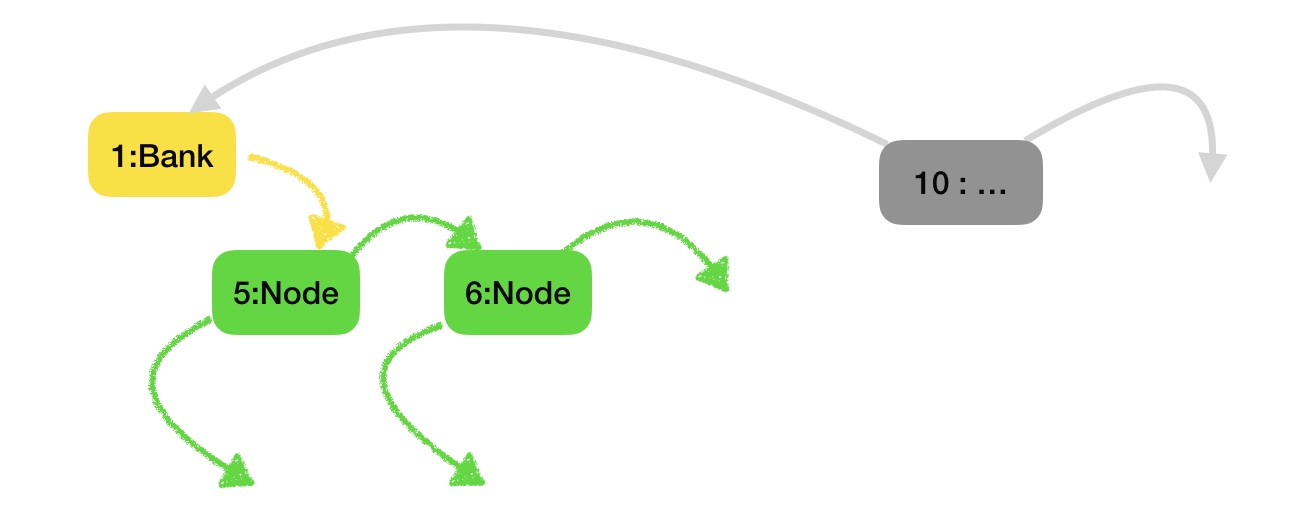
\includegraphics[width=10cm,height=4cm]{diagram2}
 \caption{Configuration from Fig. \ref{fig:Diagram} restricted to witness \{ \prg{1}, \prg{5}, \prg{6}, \prg{10} \}}
  \label{fig:DiagramRestricted}
  \end{figure}

Note that $\CanAccess{\prg{x}}{\prg{y}}$ is reflexive but  not transitive and not symmetric.

Also note the difference between $\Using{(\Future{\A})}{\prg{S}}$ and $\Future{(\Using{\A} }{\prg{S}})$.
For example,  the assertion  $\Using{(\Future{\prg{x}.\prg{f}=\prg{z}})}{\prg{S}}$ expresses that the current execution
leads to a future configuration  where
$\prg{x}.\prg{f}=\prg{z}$ will hold, and that the set \prg{S} suffices to witness this execution, while the assertion
$\Future{(\Using{{\prg{x}.\prg{f}=\prg{z}} }}{\prg{S}})$  expresses that the current execution
leads to a future configuration   where
$\prg{x}.\prg{f}=\prg{z}$ will hold and where  the set \prg{S} suffices to witness
that fact.
For example, take a configuration $\sigma$ where variable \prg{x} maps to some object \prg{31}, and where \prg{31} has a field \prg{f}
pointing to \prg{32}, and \prg{32} has a field \prg{f}
pointing to \prg{33}, and variable \prg{z} maps to  \prg{33}. Assume also that the expression to be executed in $\sigma$ starts with
\prg{x.f}=\prg{x.f.f}. Then we have that
$\M,\sigma  \models \Future{(\Using{{\prg{x}.\prg{f}=\prg{z}} }{\{\prg{x},\prg{z}\}})}$,
but
$\M,\sigma  \not\models \Using{(\Future{\prg{x}.\prg{f}=\prg{z}})}{\{\prg{x},\prg{z}\}}$.
On the other hand
$\M,\sigma  \not\models \Using{(\Future{\prg{x}.\prg{f}=\prg{z}})}{\{\prg{x},\prg{x}.\prg{f},\prg{z}\}}$

In general, for all $\M$ and $\sigma$, we have that
 $\M,\sigma \models  \Using{(\Future{\A})}{\prg{S}}$ implies $\M,\sigma \models \Future{(\Using{\A} }{\prg{S}})$, and that
 $\M,\sigma \models \Future{(\Using{\A} }{\prg{S}})$ implies that there exists a set $\prg{S}'$ such that
 $\M,\sigma \models  \Using{(\Future{\A})}{(\prg{S}\cup\prg{S'})}$.

\vspace{.2in}
We will prove that

\begin{lemma}[Preservation of validity and module linking]

$\M,\sigma \models \A$  \ \ \ then\ \ \ \   for all $\M'$ with $\M\link\M'$ is defined:\ $\M\link\M',\sigma \models \A$.
\end{lemma}




\subsection{Invariants}

We define below the meaning of invariants.\footnote{This part is as we had defined previously, with two simplifications: a) we do not need to worry about the $\obeys$-predicate here, and b) we do not distinguish the names of the classes and the names of participants in interfaces.}
The assertion $\M   \models\  \A$ requires that  the assertion $A$ is satisfied
in all reachable states.

\begin{definition}[Invariants]
\label{def:invariant}
\noindent
For a module $\M$  and assertion $\A$ we define:\\

 \begin{itemize}
 \item
$\M   \models\  \A$\ \ \  iff\ \ \ \
% $\strut\SP\SP$
$\forall \M'.\, \forall \sigma\!\in\!\Arising(\M'*\M).\ \M'*\M,\sigma \models \  \A$
 \end{itemize}
\end{definition}

The use of the set of configurations from $\Arising(\M'*\M)$ reflects that policies
 need to hold in an {\em open} world, where
we link against {\em any} module $\M'$,
about which we know nothing.

\subsection{Implication and equivalence}

\begin{definition}
\label{def:impl:equiv}
\noindent
For a module $\M$  and assertions $\A$  and $\A'$, we define strong equivalence and implication ($\equiv$ and $\sqsubseteq$), as well
as   weak equivalence and implication ($\approxeq$ and $\weakImplies$)  as follows:


 \begin{itemize}
\item
$\M   \models\  \A \strongImplies \A'$  \ \ \ \ iff \ \ \ \
$\forall \M'.\, \forall \sigma\!\in\!\Arising(\M'*\M).[\ \ \  \M'*\M, \sigma \models \A \  \ \  \longrightarrow\  \ \  \M'*\M, \sigma \models \A'\ \ \ ]$
 \item
$\M   \models\  \A \equiv \A'$ \ \ \ \ iff \ \ \ \
$\M   \models\  \A \strongImplies \A'\ \  \wedge \ \  \M   \models\  \A' \strongImplies \A$
%$\forall \M'.\, \forall \sigma\!\in\!\Arising(\M'*\M):\ \ \  \M'*\M, \sigma \models \A \  \ \longleftrightarrow\   \ \M'*\M, \sigma \models \A'$
\item
$\M   \models\   \A \weakImplies \A'$  \ \ \ \ iff \\ \ \ \ \ \ \
\strut  \hspace{1cm}  $\forall \M'.\, \forall \sigma\!\in\!\Arising(\M'*\M).\,\M'*\M, \sigma \models \A$ \  \ \  $\longrightarrow$\  \ \
$\forall \M'.\, \forall \sigma\!\in\!\Arising(\M'*\M).\,\M'*\M, \sigma \models \A'$
\item
$\M   \models\  \A \approxeq \A'$   \ \ \ \ iff \ \ \ \ \
$ \M  \models  \A \weakImplies \A' \   \ \wedge\   \  \M  \models  \A' \weakImplies \A$
 \end{itemize}
\end{definition}

The definitions from above are applicable to the empty module, eg  $\models\  \A \equiv \A'$ iff   all modules $\M$ satisfy $\M \models\  \A \equiv \A'$.
The following properties hold:

\begin{lemma}
For all modules \M, assertions \A and \A':

 \begin{itemize}
 \item
$\M   \models\  \A \equiv \A'$  \ \ \ implies \ \ \  $\M   \models\  \A \simeq \A'$
\item
$\M   \models\  \A \strongImplies \A'$  \ \ \ \ implies  \ \ \ \
$\M \models \A \weakImplies \A$
\item
$\M \models   \Using{(\Future{\A})}{\prg{S}}\ \strongImplies\ \Future{(\Using{\A} }{\prg{S}})$
\item
$ \M \models\  \Future{\A}\rightarrow \A' \  \  \weakImplies \ \ \A\rightarrow\Past{\A'}$
\item

 \end{itemize}
\end{lemma}

\paragraph{Space-Monotonicity}\footnote{Not sure how useful this concept is}

\begin{definition}[Space-Monotonicity]
We call an assertion $\A$ {\em space-monotonic} in $\M$, iff for all set expressions $\prg{S}$ and  $\prg{S}'$,
  % $\M,\sigma\models ( \prg{S} \subseteq \prg{S}'\ \wedge\  \Using{\A, \prg{S}}) \ \strongImplies\  (\Using{\A, \prg{S'}})$
%\end{definition}\footnote{If we unfold the definitions, we obtain that
% $\A$ is space-monotonic in $\M$, iff for all set expressions $\prg{S}$ and  $\prg{S}'$
 and all $\sigma\in\Arising({\M})$:
 \\
  If  $\M,\sigma\models  \prg{S} \subseteq \prg{S}'$ and $\M,\sigma\models  \Using{\A} {\prg{S}}$, then
$\M,\sigma\models  \Using{\A}{ \prg{S'}}$
\end{definition}

We prove space monotonicity for some assertions

\begin{lemma}[Space-Monotonicity for change and access]
$ ~ $

\begin{itemize}
\item
${\Changes \sE} $ is space-monotonic.
\item
$\CanAccess {\prg{x}}{\prg{y}}$ is space-monotonic.

\end{itemize}
\end{lemma}

Not all assertions  are not space-monotonic. E.g. $\forall a:\prg{Account}.\prg{a.balance}\geq 3$ is not space-monotonic.


The following lemma would be nice to have -- otherwise we will need to change the definition of monotonicity.

\begin{lemma}[Space-Monotonicity and module linking]
If $\A$ is space-monotonic with $\M$, then it is also space-monotonic with $\M*\M'$.
\end{lemma}


 \section{Specifications for Robustness Policies}

 We now use the concepts introduced in the earlier sections to specify various robustness policies

 \subsection{Specification of \Pol 2  and   \Pol 4}

We    give a formal definition of \Pol 2 and  \Pol 4, using the concepts defined earlier in  Definition \ref{def:permission}: %

\begin{definition}
\label{def:pol2}
We define  what it means for an object \prg{o} to be internal to a bank's data structure, an then define \Pol 2  and   \Pol 4  as follows:

%  \noindent
$\prg{Internal}(\prg{b})$ \ \  $\triangleq$ \ \
$\{\ \prg{o}\ \mid\  \prg{b}:\prg{Bank}\ \ \wedge \ \ (\ \prg{o} = \prg{b}\ \ \vee\  \ \prg{o}:\prg{Account}\wedge \prg{o}.\prg{myBank}=\prg{b}$\\
\strut \hspace{7.3cm} $\ \ \vee\ \ \ \exists k. \ \prg{b}.\prg{ledger}.\prg{next}^k = \prg{b})\ \ \ \ \}$


$\prg{Internal}'(\prg{a})$ \ \  $\triangleq$ \ \
$\{\ \prg{o}\ \mid\  \prg{a}:\prg{Account}\ \ \wedge \ \
 \prg{a}.\prg{myBank} :\prg{Bank}\ \wedge\  \prg{o}\in \prg{Internal}(\prg{b})\ \}$


 \vspace{.2cm}

  \Pol 2\ \  $\triangleq$ \ \
  $\forall \prg{b}.\forall \prg{S}.
  [ \ \  \prg{b}:
  \prg{Bank}\ \wedge\ \prg{this}\neq\prg{b}\ \wedge\ \ \Using{(\Future\Changes{\prg{b.currency}})}{\prg{S}} \ \ \ \ \longrightarrow \ \  $\\
   \strut $~ $ \ \ \ \hspace{1.7in}  \hfill
 $\exists \prg{o}. \ [ \ \
  \prg{o}\in \prg{S}\   \wedge\  \CanAccess{\prg{o}}{\prg{b}}\ \wedge\     \prg{o}\notin\prg{Internal}(\prg{b})  \ \ ]\ \ ]$


 \vspace{.1cm}
% \noindent
    \Pol 4\ \  $\triangleq$\ \ $\forall \prg{a}.\forall \prg{S}.\ [ \ \  \prg{a}:\prg{Account}\   \wedge\   \prg{this}\neq\prg{a} \ \wedge\ \Using{(\Future\Changes{\prg{a.balance}})}{\prg{S}}\ \ \   \
    \longrightarrow$ \\
 $\strut \hspace{3.9cm} \hfill \exists \prg{o}.\ [\, \prg{o}\in \prg{S}\ \wedge \ \CanAccess{\prg{o}}{\prg{a}}\ \wedge  \ \prg{o} \notin\prg{Internal}'(\prg{a}) \ ] \ \ \ \ ]$

\end{definition}

\paragraph{Discussion}
In other words, \Pol 2  mandates that the elements of the data structure (ie the elements from $\prg{Internal}(\prg{b})$) cannot be used (are not sufficient) to  change the currency of the bank. If a computation takes place inside the set \prg{S}, and {\em in the current state} in \prg{S}
all accesses to the bank go through elements of the data structure (ie the \prg{Account} objects),\footnote{Say why we can ignore \prg{Node} objects} then we have a guarantee that the computation will not affect the currency.
For example, if a computation takes place in the context of objects \prg{1}, \prg{2}, \prg{3}, \prg{4}, \prg{5}, \prg{7}, \prg{20} and \prg{21}, and the current receiver is no \prg{1}, then we have a guarantee that the currency of \prg{1} will not be affected. So, even through \prg{1} is involved in the computation, because there is no {\em external} access to it, we have a guaratee that the method \prg{makeAccount} will not be called on it.

An alternative way of expressing \Pol 2 is as follows:


 \Pol 2\ \  $\equiv$ \ \
  $\forall \prg{b}.\forall \prg{S}.
  [ \ \  \prg{b}:
  \prg{Bank}\ \wedge\   \prg{b}\neq\prg{this}\ \wedge\  \forall \prg{o} \in \prg{S}.\, [\ \prg{o}\in\prg{Internal}(\prg{b}) \ \vee\  \neg  \CanAccess{\prg{o}}{\prg{a}}  \ \ ]$
\\ \hfill \strut $~   \ \ \ \hspace{1.7in}  \  \ \longrightarrow \ \ \ \neg(
 \Using{(\Future\Changes{\prg{b.currency}})}{\prg{S}})\   \  \ \ ]$

\vspace{.01in}
% TO\_DO: discuss the difference between  $\Using{(\Future\Changes{\prg{b.currency}})}{\prg{S}})$, and
% $\Future{(\Using{\Changes{\prg{b.currency}}{\prg{S}})}}$.

\vspace{.01in}
\Pol 2  guarantees
that if an object \prg{o}$\neq$\prg{b} may affect the value of \prg{b.Currency} only if the  objects
involved in the process of affecting the value of \prg{b.Currency}  include at least an object $\prg{o}'$
which had direct access to \prg{b}, and
whose class is  not  \prg{Account}. Stated positively, this policy mandates
that exporting an \prg{Account} to an environment will not affect the \prg{Currency} of \prg{b}.
In other words,
\prg{Account}s protect the integrity of the \prg{Bank}'s currency.


In more detail, by applying  Definition \ref{def:invariant} on Definition \ref{def:pol2}, the  meaning of policy \Pol 2
  is, that a runtime configuration $\sigma$ satisfies  \Pol 2  if whenever the current receiver in $\sigma$
 is not a \prg{Bank} object, and the execution of $\sigma$ leads to another runtime configuration $\sigma'$
 with a different value for \prg{b.Currency}, then the objects involved in the execution from
 $\sigma$ to $\sigma'$ include at least one object which had direct access to \prg{b}.
 Note that this direct access needs to exist at the beginning of   the execution, \ie at $\sigma$.
 Formally:

 \noindent
 $\M, \sigma \models  \Pol 2$\\$ \strut \ \ \ \  \ \  \longleftrightarrow $\\
 $\forall \prg{b}.\forall S.\ [ \ \ \ \ \M, \sigma \models \prg{b}:\prg{Bank}\ \wedge\
 \sigma(\prg{b})\neq \ \sigma(\prg{this}) $\\
 $\strut \hspace{2.1cm}  \wedge \
 \ \exists\sigma'.(\ \ \ \ \M, \sigma\mid_S \leadsto^* \sigma'\
\ \wedge\ \interp {\prg{b.Currency}}{\M,\sigma}\neq \interp {\prg{b.Currency}}{\M,\sigma'[\prg{b}\mapsto\sigma(\prg{b})]}\ )$\\
$\strut \hspace{4.7cm} \longrightarrow$ \\
 $\strut \hspace{2.7cm}  %\exists \prg{o}. (\ \  \sigma(\prg{o}) \!\!\in\!\!\prg{S}\ \
 \exists \prg{o}. (\ \ \prg{o} \!\in\!S\ \
  \wedge \ \ \M, \sigma \models \CanAccess{\prg{o}}{\prg{b} }\ \wedge \  \prg{o}\notin \prg{Internal}(\prg{b}) \   \ ) \ \ \ \ \ \ \  ]$



\subsection{Specifying  "no leaks"}

This is a family of guarantees that Dean seemed especially interested in, when we discussed in March in London.
For the particular example, we want to express that

\begin{description}
\item[\Pol 7]
The \prg{Bank} does not leak out of the \prg{Bank}/\prg{Account} system
%\item[Pol\_7]
%The \prg{Accounts} do  not leak out of the \prg{Bank}/\prg{Account} system
\end{description}

And we give a formal specification

\begin{definition}[Banks do not leak]
\label{def:bankNoLEak} We define \Pol 7 as follows:

\Pol{7}\ \  $\triangleq$\ \ $\forall \prg{b}.\forall \prg{S}.\ [  \ \ \prg{b}:\prg{Bank}\ \wedge\  \prg{o}:\prg{Object}\  \wedge\   \neg(\CanAccess{\prg{o}}{ \prg{b}})\ \wedge\   \Using {(\Future{\CanAccess {\prg{o}}{\prg{b}}})} {\prg{S}} $
 \\  $\strut$ \hspace{4cm}
  $\longrightarrow$
 $\strut \hspace{0.5cm}  \exists \prg{o}'.\ [\, \prg{o}'\in \prg{S}\ \wedge \  \CanAccess{\prg{o}'}{ \prg{b} }\ \wedge\   \prg{o}' \notin \prg{Internal}(\prg{b}) \, ) \ ] \  \  \ \  ]$

%\hspace{.1cm}
%{\bf {Pol\_8}}\ \  $\equiv$\ \ $\forall \prg{o},\prg{b}, \prg{o}'\forall \prg{S}.\ [  \ \ \prg{b}:\prg{Bank}\ \wedge \prg{o}\in\prg{Internal}({\prg{b}})\ \wedge\  \prg{o}':\prg{Object}\ \ \neg(\CanAccess{\prg{o}'}{ \prg{o}})\ \wedge\   \Using {(\Future{\CanAccess {\prg{o}'}{\prg{o}}})} {\prg{S}} $
% \\  $\strut$ \hspace{4cm}
%  $\longrightarrow$
% $\strut \hspace{0.5cm}  \exists \prg{o}''.\ [\, \prg{o}''\in \prg{S}\ \wedge \  \CanAccess{\prg{o}''}{ \prg{o} }\ \wedge\   \prg{o}'' \notin \prg{Internal}(\prg{b}) \, ) \ ] \  \  \ \  ]$
\end{definition}

In other words, \Pol 7 guarantees that objects that are internal to the bank \prg{b} do not leak access to it.
In more detail: if   objects  \prg{o} and \prg{b} exist  now, and \prg{o} does not have direct access to \prg{b} now, but obtains
access to \prg{b} through some computation which involves objects from the set \prg{S}, then at least one  object  from \prg{S} has
now direct access to   \prg{b} and this object is not internal to \prg{b}.

\section{Adherence to Policies}
\label{section:Adherence}
In this section we will outline the proofs that particular modules adhere to their specifications.
This serves to demonstrate the practicality of our approach.
In particular we will show two different versions fo the \prg{Bank}/\prg{Account} example (sections \ref{section:Adherence:ModuleOne} and \ref{section:Adherence:ModuleTwo}, and we will prove that
both satisfy the policies \Pol 2, \Pol 4, and \Pol 7, while they differ in the definition of \prg{Internal}.
But before doing that, in section \ref{section:GeneralPropertiesExecution}, we will study some further properties of execution.


\subsection{General properties of execution}\footnote{Find better title?}
\label{section:GeneralPropertiesExecution}

We will first define some further predicates which reflect over the program execution and prove
some general properties of program execution.

We call a locations set, \prg{L}, an expression which denotes a set of addresses and field identifiers, \eg, $\{\ (\prg{b},\prg{ledger}), (\prg{b}.\prg{ledger},\prg{balance})\ \}$ is such a locations set.

\begin{definition}[Framing]
Take arbitrary module \M, assertion \A, , ...

\begin{itemize}
\item
\interp{\prg{L}}{\sigma,\M*\M'} = ....
\item
$ \sigma\mid _L$ ....
\item
$\M, \sigma \models \prg{L} \frames \prg{e}$\ \ \ \  \ iff \ \ \ \ \
$\forall \M'.\forall \sigma'\!\in\!\Arising({\M*\M'}). \forall L.$\\
\strut \hspace{1cm} $  [ \ \ L=\interp{\prg{L}}{\M,\sigma}\, \wedge\,
 \sigma\mid _L= \sigma'\mid_L \ \   \longrightarrow\ \ \   \interp {\prg{e}}{\sigma,\M*\M'}  =  \interp {\prg{e}}{\sigma',\M*\M'}
\ \ ]$
\item
$\M  \models \prg{L} \frames \prg{e}$\ \ \ \  \ iff \ \ \ \ \
$\forall \M'.\forall \sigma\!\in\!\Arising({\M*\M'}). \ \M'*\M, \sigma \models \prg{L} \frames \prg{e}$
\item
$\M, \sigma \models \prg{L} \frames\A $\ \ \ \  \ iff \ \ \ \ \
$\forall \M'.\forall \sigma'\!\in\!\Arising({\M*\M'}). \forall L.$\\
\strut \hspace{1cm} $ [ \ \ L=\interp{\prg{L}}{\M,\sigma}\, \wedge\,
\sigma\mid _L= \sigma'\mid_L \ \   \longrightarrow\ \ \   [\ \M*\M',\sigma \models \A   \ \longleftrightarrow\ \M*\M',\sigma' \models \A
\ \ ] $
\item
$\M  \models \prg{L} \frames \A$\ \ \ \  \ iff \ \ \ \ \
$\forall \M'.\forall \sigma\!\in\!\Arising({\M*\M'}). \ \M'*\M, \sigma \models \prg{L} \frames \A$
\end{itemize}

\end{definition}

NOTE\_TO\_SELF: we need to think about whether we also need to make \prg{L} self-framing.
Also, rethink whether we need to stick new modules $\M'$ to the whole thing.
--
Also, the sets are not equal -- they are isomorphic. We can deal with isomorphisms, but
it has a high notation penalty. Can we pretend that they are equal? hmhhhhh


And then we can prove that changes in the interpretation or the validity require a change in the frame:

\begin{lemma}[Change in the context of framing]
Take arbitrary module \M, assertion \A, such that  $\sigma\in\Arising({\M*\M'})$

\begin{itemize}
\item
If  $\M  \models \prg{L} \frames \prg{e}$, and
$\M'*\M, \sigma \models \Using{(\Future{\Changes{\prg{e}}})}{\prg{S}}$, \\
then there exists a pair $(\prg{e}',\prg{f})$ , with
$\M,\sigma \models (\prg{e}',\prg{f})\in \prg{L}$\footnote{Sophia, you need to check this bit  what if \prg{z}
there is no handle in \prg{L}, eg what if \prg{L} talks about anonymous objects
\eg \prg{L} = $\{ o \ \mid o.\prg{myBank}=\prg{b} \}$?Here $o$ is anonymous. Also, do we need $\M$ or $\M'*\M$?}
and $\M'*\M, \sigma \models  \Using{\Future{\Changes{\prg{e}'.\prg{f}}}}{\prg{S}}$

\item
similar for
$\M'*\M, \sigma \models \Using{\Future{\Changes{\A}}}{\prg{S}}$
\end{itemize}

\end{lemma}

\begin{figure}[tbp]
\begin{lstlisting}
 class Bank {
   private field ledger;   // a Node

   Bank( )
     { ledger = null; }
   fun makeAccount(amt)
     { account = new Account(this);
       ledger = new Node(account, amt, ledger);
       return account; }
   fun deposit(source, destination, amnt)
     { sourceNd = ledger.getNode(source)
       destinationNd = ledger.getNode(destination)
       if (sourceNd!=null && destinationNd!=null && sourceNd.balance>amt) then
          { < sourceNd.balance = sourceNd.balance-amt
              destinationNd.balance = destinationNd.balance+amt > }
        else
          { return }               }
 }

 class Account {
   private field myBank;  // a Bank

   Account(aBank)
     { myBank = aBank;  }
   fun sprout( )
     // create Account in same Bank with 0 balance
     { return this.myBank.makeAccount(0)  }
   fun deposit(source, amnt)
     // if destination is an Account in myBank,  and  source holds enough money,
     // then transfer amnt from source into receiver
     { myBank.deposit(source,this,amnt) }
 }

  class Node{
   field balance;     // the  money held in theAccount a number
   field next;        // the next node
   field theAccount;  // the account

   fun getNode(account)
     { if (theAccount==account) then
           { return this }
       elseif (next!=null)
           { next.getNode(account) }
       else
           {  return null }            }	
 }
\end{lstlisting}
\caption{\MOne: First version of the Bank example, in detail}
\label{fig:BankDetailedOne}
 \end{figure}


We now think a bit more about changes in accessibility. The predicate  $\Gives(\prg{x},\prg{y},\prg{z})$ expresses
that \prg{x} passed to \prg{y} access to \prg{z}.

\begin{definition}[Giving]
For arbitrary module \M and $\sigma$, we define:

\begin{itemize}
\item
$\M,\sigma  \models \Gives(\prg{x},\prg{y},\prg{z})$\ \ iff \ \
$\sigma(\prg{this})$=$\sigma(\prg{x})$ \  $\wedge$ \
$\M, \sigma \models \neg (\MayAccess( \prg{y},\prg{z})\,)$ \ $\wedge$ \\
\strut \hspace{.9cm} $\exists \sigma'. \ [\  \M,\sigma \leadsto \sigma'  \  \wedge  \
 \M,\sigma' \models \MayAccess( \prg{y},\prg{z})\ ]$
\end{itemize}

\end{definition}

The following lemma says that any changes in accessibility witnessed\footnote{is that the right term? or frames?}
by set \prg{S} is due to an element of \prg{S} giving the object.

\begin{lemma}[Change in Accessibility is caused by Giving]
For any module \M, and  $\sigma$

\begin{itemize}
\item
If  $\M, \sigma  \models \neg(\MayAccess(\prg{y},\prg{z}))$, and
$\M, \sigma \models \Using{(\Future \MayAccess(\prg{y},\prg{z}))}{\prg{S}}$, \\
 then there exists a  $\prg{x}$  and  $\prg{y}'$, with
%$\M,\sigma \models  \prg{e} \in \prg{S}$, and
$\M,\sigma \models \Using{(\Future{\Gives(\prg{x},\prg{y}',\prg{z})})}{\prg{S}}$.
\end{itemize}

\end{lemma}

\subsection{Adherence to Policies for module \MOne}
\label{section:Adherence:ModuleOne}

In figure \ref{fig:BankDetailedOne} we show the  code for \MOne in detail.

\subsubsection{\MOne~preliminaries}
We define the footprint of \prg{b.balance} as

\begin{definition}We define the currency-footprint of a bank as follows:

$\prg{CurrencyFootprint}(\prg{b})$ $\triangleq$
$\{ \ (\prg{b},\prg{ledger}) \} \ \cup$\\
\strut \hspace{4.8cm}
$\{ \ (\prg{o},\prg{balance})\ \mid \exists k:\mathbb{N}. \prg{x}.\prg{ledger}.\prg{next}^k=\prg{o} \ \}$
\end{definition}

\begin{lemma}
$\MOne \models \prg{b}:\prg{Bank} \rightarrow \prg{CurrencyFootprint}(\prg{b}) \frames \prg{b}.\prg{currency}$
\end{lemma}

We also define a predicate $Gives(prg{x},prg{y},prg{z})$ which expresses that while \prg{x} was excuting, it
passed to \prg{y} access to \prg{z}.
... more in handwritten notes ...

\subsubsection{\MOne~adheres to \Pol 2}
\begin{lemma}
$\MOne \models \Pol 2$
\end{lemma}
Proof sketch   in Sophia's handwritten notes.

\subsubsection{\MOne~adheres to \Pol 4}

\begin{lemma}
$\MOne \models \Pol 4$
\end{lemma}

\subsubsection{\MOne~adheres to \Pol 7}

\begin{lemma}
$\MOne \models \Pol 7$
\end{lemma}
Proof sketch  in Toby's handwritten notes.

\subsection{Adherence to Policies for module \MTwo}
\label{section:Adherence:ModuleTwo}

In figure \ref{fig:BankDetailedTwo} we show the  code for \MTwo in detail.

\begin{figure}[tbp]
\begin{lstlisting}
 class Bank {    }

 class Account {
   protected field balance; // the data of the Account;
   protected field myBank;  // a Bank

   Account(aBank,amt){
     balance = amt;
     myBank = aBank }

   fun deposit(source, amnt){
     if ( myBank== source.myBank && source.balance>=amt && amt>0) then
        { source.balance = source.balance-amt;
           this.balance = this.balance + amt }    }
}

\end{lstlisting}
\caption{\MTwo: Second version of the Bank example, in detail}
\label{fig:BankDetailedTwo}
 \end{figure}

We give the code for \MTwo~ in Figure ???, and define \prg{Internal} as follows.
The code works through ...
The set  \prg{Internal} describes ....


\subsubsection{\MTwo~adheres to \Pol 2}

\subsubsection{\MTwo~adheres to \Pol 4}

\subsubsection{\MTwo~adheres to \Pol 7}


\section{Hoare Logic}
\label{section:Hoare}
Here we give Hoare Logic rules which allow us to prove adherence to policies.
NOTE: Not sure when we will get to do these rules. If we get to define these rules, then we will use them for the proofs
 in section \ref{section:Adherence:ModuleOne}
and we will swap section \ref{section:Adherence} and section \ref{section:Hoare}

\section{Further Applications}
In this section we will apply our methodology to give specifications to other famous patterns from the OCAP literature,
\ie the membrane, the DOC-tree, and ...

\subsection{The DOM tree}
....

\subsection{The membrane}
...

\subsection{Sealer/Unsealer}

In Figure \ref{fig:WrapUnwrap} we visit the sealer/unsealer example  from cite-Morrison and Miller.


\begin{figure}[tbp]
\begin{lstlisting}
 class Box{
   ...
   fun seal(element){... }
   fun unseal(sealed){ ... }
 }

\end{lstlisting}
\caption{Wrapping and Unwrappingl}
\label{fig:WrapUnwrap}
 \end{figure}

The specification of these functions mandates \prg{seal} wraps the object into another structure, and \prg{unseal} unwraps the original object out of the structure, Like cite(David Swasey, OOPLSA'13), we use an uninterpreted  predixate, $\prg{Wrapped}(\prg{z},\prg{o},\prg{b})$ which expresses that \prg{z} contains the value of \prg{o} as wrapped by \prg{b}.

The policies from below express that \prg{seal} wraps an object, while \prg{unseal} unwraps it, and they are very similar to those from cite(David Swasey, OOPLSA'13).

\Pol {seal\_1} $\triangleq$
\strut \hspace{2.1cm} $\prg{o}:\prg{Object}\ \wedge\ \prg{b}:\prg{Box}$  \\
\strut \hspace{6cm}$\{\ \prg{x} = \prg{b}.\prg{seal}\prg{(o)}\ \}$\\
\strut \hspace{5cm} $\prg{Wrapped}(\prg{x},\prg{o},\prg{b})$

\hspace{.1cm}

\Pol {seal\_2} $\triangleq$
\strut \hspace{2.2cm}$\prg{o}:\prg{Object}\ \wedge\ \prg{b}:\prg{Box}\  \wedge\  \prg{Wrapped}(\prg{x},\prg{o},\prg{b})$\\
\strut \hspace{6cm}$ \{\ \prg{y} = \prg{b}.\prg{unseal}\prg{(x)} \}$\\
\strut \hspace{5cm} $\prg{y}=\prg{o}$

\hspace{.1cm}

But further to the specification from cite(David Swasey, OOPLSA'13) ,
we want to also express that the {\em only} way to extract a sealed object
 out of its box, is by calling the \prg{unseal} function on the box. For this, we
 define an assertion $\prg{Sealed}(\prg{o})$ which expresses that {\em all} accesses to \prg{o}
go through some sealed box, and the assertion $\prg{UnSealed}(\prg{o})$ which expresses that the object can be accessed without
going through a sealed box. Using these predicates, in  \Pol {seal\_3} we express that if a sealed object
becomes unsealed, then this must have happened though a call to the \prg{unseal} function:



$\prg{Sealed}(\prg{o}) \  \triangleq\ \prg{o}:\prg{Object}\ \wedge$\\
\strut \hspace{2.75cm}$ \forall \prg{o}':\prg{Object}.\ [ \ \CanAccess{\prg{o}}{\prg{o}'}\ \wedge \prg{o}\neq\prg{o'}\ \rightarrow\ \exists \prg{b}:\prg{Box}.\prg{Wrapped}(\prg{o}',\prg{o},\prg{b})\ ]$

$\prg{Unsealed}(\prg{o}) \  \triangleq\ \neg \prg{Sealed}(prg{o})$

\hspace{.05cm}

\Pol {seal\_3} $\triangleq$  $\forall \prg{o}.\forall{\prg{S}}.$ \ \
% $\\ \strut \hspace{4cm} $
$[\ \ \Using{(\, \prg{Sealed}(\prg{o}) \ \wedge\ {\Future{\prg{Unsealed}({\prg{o}})}}\, )}{\prg{S}} \ \ \ \longrightarrow $\\
\strut \hspace{8cm}$ \exists \prg{b},\prg{x}.[ \prg{b},\prg{x}\in\!\prg{S}\ \wedge\   \prg{Wrapped}(\prg{x},\prg{o},\prg{b}) \ \wedge$\\
\strut \hspace{9cm}$\Using{(\Future{\Calls{\prg{b.unseal}(\prg{x})}})}{\prg{S}}\ ]
$\footnote{This definition is not perfect, as it does not preclude that the call to $\prg{b.unseal}(\prg{x})$ could happen {\em after}
\prg{o} became \prg{Unsealed}. Perhaps, we should instead have an assertion combinator ${\A\, \kw{to} \A'\,\kw{caused by} \prg{code}}$, and we could then say:

\Pol {seal\_3} $\triangleq$  $\forall \prg{o}.\forall{\prg{S}}.$ \ \
% $\\ \strut \hspace{4cm} $
$[\ \ (\Using{{\prg{Sealed}(\prg{o})}}{\prg{S}}) \  \kw{to}\  (\Using{\prg{Unsealed}({\prg{o}})}{\prg{S}})\ \kw{caused\,by}\  \prg{b.unseal}{(\prg{x})} \ ]$
}




\subsection{The DAO }

We describe here only some aspects of the DAO contract.
The DAO keeps a table called \prg{balances} which keeps track of the balances for all its clients.
 The following three policies mandate that \Pol {DAO\_1}: the contents of \prg{o.balances} can only be affected by \prg{o}
 itself, that \Pol {DAO\_2}: the ether held in the DAO is the sum of the balances in all its participants, and \Pol {DAO\_3}: that any
 participant can withdraw up to amount that the the DAO holds for it.
 In fact, with \Pol {DAO\_2} is too strong, \Pol {DAO\_1} and \Pol {DAO\_3} are not, and any
 contract adhering to these two policies would have not suffered from the DAO-attack\cite{...}.


In the below we also have the use a lookup function $\Caller$ with obvious meaning\footnote{we can define it with what we have}.

~ \\
\noindent
$\Pol {DAO\_1}$ $\triangleq$ $ ...\ \Changes{\prg{dao.balances(o)}}\  \longrightarrow\   \Caller=\prg{o} ....$

~ \\
\noindent
$\Pol {DAO\_2}$ $\triangleq$ $ ... \prg{dao.ether}=\sum_{o\in dom(\prg{dao.balances})}  \prg{dao.balances(o)}$

~ \\
\noindent
$\Pol {DAO\_3}$ $\triangleq$ $... \ \prg{dao.balances(o)}=m \ \wedge\ \Caller = \prg{o}\ \wedge\ \Calls{payme} \ \wedge\ \prg{x}=m'\leq m  \longrightarrow  $\\
\strut \hspace{5cm}
$\Future{(\Caller=\prg{dao}\ \wedge\ \Calls{send} \ \wedge\  \prg{x}=m')}$\footnote{SOPHIA: Here is a point where we
want the parameters to have the meanings as in the future configuration! Easy to fix- stick in the calls names for the arguments}

Note that $\Pol {DAO\_3}$ is a liveness property. It promises that if one of the \prg{DAO} participants asks to be paid back
(by calling \prg{payMe}), then eventually they will get their money back (in the future the \prg{DAO} will call the function \prg{send}
with the appropriate ether argument).


\section{Discussion}
In this section we compare ``classical'' specifications with those proposed here\footnote{shall we call them ``holistic''?}

\begin{itemize}
\item Classical specifications reflect over (\ie mandate properties of) the state of the execution now, while
holistic specifications can also reflect over the possible  states   reachable from now, or those states in the past
which lead to the current state.

\item Classical specifications describe what happens under {\em correct} use  of the data structure,
while holistic specifications  describe preservation of properties under {\em arbitrary} use  of the data structure.

\item Both specifications employ notions of footprint\footnote{In separation logic, and also others}, but
classical footprints are related to the carrier set\footnote{Witness??} of properties in the current state, while
because  of the temporal operators  of holistic specs, holistic witnesses\footnote{not sure whether witness of footprints}
 can  also talk about the carrier sets\footnote{Witness??} of arbitrary executions.
 Also, holistic witnesses are first order\footnote{I expect that in some sep logic they are first order too, but perhaps we
 can compare with the first version of sep logic}

% \item Classical specifications describe the effects of code execution, while holistic specs also reflect over
 %describe the causes of -- this is related to the next item
%  arbitrary effects, such as $\Future{\Changes{\prg{e}}}$.


\item Classical specifications describe sufficient conditions, while holistic specifications also describe necessary conditions. 
Namely, the assertion  $\A \rightarrow \Future{\A'}$ says that $\A$ is a {\em sufficient} condition to achieve the
effect $\A'$ in the future, while $(\Future{\A'}) \rightarrow \A$ says that $\A$ is a {\em necessary} condition to achieve $\A'$ in the future.

\item Defensive Programming Rather than
      "What can the others (client) achieve using my code"
Say
     "What do I prevent the others from doing with my objects"

 \item
 From KVM paper: From the KVM paper

"Contract interactions are often complex, with safe contracts able to have their guarantees violated by calling into potentially malicious and unknown third party contract code."

Rather than say
    What can the others expect from me
We say
    What do I have to make sure the others cannot do with my objects

Elias
    Modularity is the ability to ...

    In order to deduce that xxx I must lookat the spec of yyy methods/

    Has modular verif gone too far?

Modular verification should not imply modular specifications

\end{itemize}


 



\subsection*{LATEX mysteries and terminology}
 \begin{enumerate}
 \item
 How can we make the references refer to the Definitions, Lemmas etc
 rather than the section where these appear?
 \begin{quotation}
   \color{orange} KJX:   Not sure what the problem is. I've put labels
   in the definitions and I can use refs to get definition
   numbers~\ref{defONE} and~\ref{def:syntax:classes} ---
   not ~\ref{secONE} and ~\ref{sec:syntax:classes}, the section
   numbers containing those definions.

   Alternatively there is the ``cleveref'' package
   \url{http://tug.ctan.org/tex-archive/macros/latex/contrib/cleveref/cleveref.pdf}
   where a ``\verb+\cref{foo}+'' can generate both the type and the
   numbner e.g.  ``Definition 3''.
 \end{quotation}

 \item
 Need a nice metavariable for set of addresses, currently it is $R$. Perhaps instead use an enumeration, as eg $\{ \ \alpha_1,...\alpha_n\ \} $
 or $\kappa$?

 \begin{quotation}
 \color{orange} KJX: Hmm, the enumeration is fine. Otherwise $A$?
 $\mathcal{A}$?  Or we could call that set a ``footprint'' and so go
 with $F$ or $\mathcal{F}$\ldots
 \end{quotation}
\item
Find a nice term  to refer to module pairs  (internal, external), and a term for
our version visible states semantics.
 \begin{quotation}
   \color{orange} KJX: ``modules'' and ``modular state semantics''.
   Going to ``modules'' only makes sense with my answer below.
   Other permutations of
   ``visible module/modular state semantics'' work also work:
     modular visible state; visible modular state; etc\ldots
 \end{quotation}


\item
Better symbols for module linking (currently a $\M\link\M'$), and
for module pairing (currently a $\M\mkpair \M'$) -- perhaps there should not be such an operator, as
it does not create a new module, it is only used in execution ($\M\mkpair \M', \sigma \leadsto \sigma'$)
and in satisfaction of assertions ($\M\mkpair \M', \sigma\models \A$).
\footnote{\toby{TM: I like~$\M \mkpair \M'$ as it suggests the asymmetry of the visible
    state semantics wrt~$\M$ and~$\M'$.}}

 \begin{quotation}
   \color{orange} KJX: I'm so used to $\M\link\M'$ that I can't think
   of an alternative --- or do I recall we used $\M * \M'$ as a
   separating conjunction?

   So I really liked $\M\mkpair \M'$ --- except then I though that I
   couldn't remember which was the module (inside) and which the
   anti-module (the outside).  For some reason I thought outside would
   go first.  Then I realised, it's easy, cos $\M$ is always the
   module, and $\M'$ is the antimodule.

   At which point I though: OK so let's just write $\M$ as the module,
   and given any $\M$, then $\M'$ (or $\overline{\M}$ or I guess
   \textbf{out}($\M$)) for the antimodule.

   The only thing I think this loses is that the $\M\mkpair \M'$
   syntax, also like a seperating conjunction, is sort of
   self-framing: $\M\mkpair \M'$ encompasses the universe of modules.
   Whereas the other way around, we'd need a (implicit) universe of
   all modules $\mathcal{U}$, and then define $\M' \triangleq
   \mathcal{U} - \M$  If we went with $\M'$ then Sophia couldn't use
   $\M''$ and friends --- have to write \texttt{N} and \texttt{O} for other
   modules?

   I think the only change I could see in the whole document was that
   lemma~\ref{lemma:module_pair_execution} is subsumed into
   lemma~\ref{lemma:linking:properties}.
 \end{quotation}


 \end{enumerate}
